%Auteurs : Nicolas Englebert
\documentclass[british,french,11pt, a4paper, openany]{book}

% Règles de bonne pratiques :
% https://fr.wikibooks.org/wiki/LaTeX/Gestion_des_gros_documents

%%%%%%%%%%%%%%%%
%%% Packages %%%
%%%%%%%%%%%%%%%%

%%% Compatibilité %%%
\begingroup\expandafter\expandafter\expandafter\endgroup
\expandafter\ifx\csname IncludeInRelease\endcsname\relax
\usepackage{fixltx2e}
\fi 					% Si version LaTeX < 2015, inclut un fix.

%%% Général %%%
\usepackage[utf8]{inputenc}
\usepackage{babel}
\usepackage{lmodern}
\usepackage[T1]{fontenc}
\addto\extrasfrench{\sisetup{locale = FR,detect-all}} % Switch siunitx en fonction de la langue babel :)
\addto\extrasbritish{\sisetup{locale = UK,detect-all}}
\usepackage{courier}
\usepackage{graphicx}
\usepackage{cancel}

%%% Tableau %%%
\usepackage{tabularx} %Permet d'auto dimensionner les tableaux



%%% Bibliographie %%%
\usepackage[style=alphabetic,backend=biber]{biblatex}
\usepackage[autostyle]{csquotes}
\DeclareNameAlias{sortname}{last-first}
\DeclareFieldFormat{url}{\space\url{#1}}
\DeclareNameAlias{labelname}{last-first}
%\addbibresource{sample.bib}


%%% Graphiques %%%
\usepackage{tikz}
\usepackage{pgfplots}
\usepackage{circuitikz}

%%% Mise en page %%%
\usepackage{mathtools}
\usepackage{amssymb}
\usepackage{bbm}
\usepackage{amsthm}
\usepackage[tt]{titlepic}% Centre le titre
\usepackage{fancyhdr}   % Permet de modifier l'entête & footer
\usepackage{caption}     % Permet d'ajouter des légendes en images sans les mettre en float + dans la marge + ref vers le haut de l'envirronement
\usepackage{wrapfig}
\usepackage{fullpage}
\usepackage{multicol}   % pour les liste sur plusieurs colonnes
\usepackage{subfigure}  % alligne deux images cote a cote
\usepackage{float}      %permet de mettre du texte entre les figures grace a [H]. Génial! 
\usepackage{eso-pic}    % Fond d'écran page de garde
\usepackage{adjustbox}  % Empêche les box de sortir de la page


%%% Math %%%
\usepackage{delarray} % Belles matrices
\usepackage{siunitx}


%%% Codes %%%
\usepackage{listings}
\usepackage[final]{pdfpages} %% Inclusion fichier pdf

%% Reference
\usepackage{hyperref}
\renewcommand*{\figureautorefname}{fig.}
\def\appendixautorefname{annexe}
\def\tableautorefname{tab.}
\renewcommand*{\chapterautorefname}{ch.}
\newcommand{\subfigureautorefname}{\figureautorefname}



%%%%%%%%%%%%%%%%%
%%% Commandes %%%
%%%%%%%%%%%%%%%%%

%%% Physique %%%
\newcommand{\cst}{\text{cst}}
\newcommand{\D}{\partial}
\newcommand{\E}{\vec E}
\newcommand{\B}{\vec B}
\newcommand{\F}{\vec F}
\newcommand{\modu}[1]{|$#1$|}

%%% Math %%%
\newcommand{\oiint}{\int\!\!\!\!\!\!\! \:\!\subset\!\!\supset\!\!\!\!\!\!\!\int}
\newcommand{\rot}{\text{rot}\,}
\newcommand{\divv}{\text{div}\,}
\newcommand{\phas}[1]{\underline{#1}}
\newcommand{\RE}{\text{Re}}
\newcommand{\ft}{\overset{\mathcal{F}}{\longleftrightarrow}}
\newcommand{\lt}{\overset{\mathcal{L}}{\longleftrightarrow}}
\newcommand{\DS}{\displaystyle}
\newcommand{\Tr}{\text{Tr }}



%% Box
\shorthandon{:}
\newcommand{\theor}[1]{\adjustbox{minipage=\linewidth-2\fboxsep-2\fboxrule,fbox}{\textsc{\iflanguage{british}{Theorem}{Théorème}: }#1}}
\newcommand{\defi}[1]{\adjustbox{minipage=\linewidth-2\fboxsep-2\fboxrule,fbox}{\textsc{\iflanguage{british}{Definition}{Définition}: }#1}}
\newcommand{\lemme}[1]{\adjustbox{minipage=\linewidth-2\fboxsep-2\fboxrule,fbox}{\textsc{\iflanguage{british}{Lemma}{Lemme}: }#1}}
\newcommand{\prop}[1]{\adjustbox{minipage=\linewidth-2\fboxsep-2\fboxrule,fbox}{\textsc{\iflanguage{british}{Property}{Propriété}}\\ #1}}
\newcommand{\proposition}[1]{\adjustbox{minipage=\linewidth-2\fboxsep-2\fboxrule,fbox}{\textsc{Proposition}\\#1}}
\newcommand{\cadre}[1]{\adjustbox{minipage=\linewidth-2\fboxsep-2\fboxrule,fbox}{#1}}
\newcommand{\retenir}[1]{\adjustbox{minipage=\linewidth-2\fboxsep-2\fboxrule,fbox}{\textbf{\textit{\textsc{\iflanguage{british}{To remember}{À retenir}}: }}#1}}

\newcommand{\corollaire}[1]{\bigbreak\begin{tabular}{||c}
	\begin{minipage}{\textwidth}
		\textsc{\iflanguage{british}{Corollary}{Corollaire}: } \textit{#1}
	\end{minipage}
	\end{tabular}}
\newcommand{\exemple}[1]{\bigbreak\begin{tabular}{|c}
	\begin{minipage}{\textwidth}
		\textsc{\iflanguage{british}{Example}{Exemple}: } #1
	\end{minipage}%
	\end{tabular}}%
\shorthandoff{:}
    

%\pagestyle{headings} % Titre du ch et numéro page dans l'entete
\renewcommand{\proofname}{Démonstration}
\addto\captionsfrench{\def\tablename{Tableau}}


%%% Background %%%
\newcommand\BackgroundPic{%
	\put(0,0){%
		\parbox[b][\paperheight]{\paperwidth}{%
			\vfill
			\centering
			
\includegraphics[width=\paperwidth,height=\paperheight,%
			keepaspectratio]{../../Builder/ulb.jpg}%
			\vfill
}}}

%%% Annexes Cedu %%%
%\usepackage{calrsfs}
\DeclareMathAlphabet{\pazocal}{OMS}{zplm}{m}{n}
\usepackage{fourier-orns}

\setlength{\parindent}{0pt} 

%%% Attributs %%%
\newcommand*{\NomduCours}[2]{\def\cours{#1}\def\memo{#2}}
\newcommand*{\annee}[2]{\def\adebut{#1}\def\afin{#2}}

\newcounter{auteurcnt}
\newcommand\addauteur[2]{%
	\stepcounter{auteurcnt}%
	\csdef{auteur\theauteurcnt}{\mbox{#1~\textsc{#2}}}}
\newcommand\getauteur[1]{%
	\csuse{auteur#1}}

\newcounter{illustrateurcnt}
\newcommand\addillustrateur[2]{%
	\stepcounter{illustrateurcnt}%
	\csdef{illustrateur\theillustrateurcnt}{\mbox{#1~\textsc{#2}}}}
\newcommand\getillustrateur[1]{%
	\csuse{illustrateur#1}}

\newcounter{rappeltheocnt}
\newcommand\addrappeltheo[2]{%
	\stepcounter{rappeltheocnt}%
	\csdef{rappeltheo\therappeltheocnt}{\mbox{#1~\textsc{#2}}}}
\newcommand\getrappeltheo[1]{%
	\csuse{rappeltheo#1}}

\newcounter{professeurcnt}
\newcommand\addprofesseur[2]{%
	\stepcounter{professeurcnt}%
	\csdef{professeur\theprofesseurcnt}{\mbox{#1~\textsc{#2}}}}
\newcommand\getprofesseur[1]{%
	\csuse{professeur#1}}

\newcounter{iter}
\usepackage{paracol}
% Attributs
\NomduCours{Circuits logiques et numériques}{ELEC-H-305}
\addauteur{Cédric}{Hannotier}
\addprofesseur{Dragomir}{Milojevic}
\annee{2015}{2016}

% Document
\begin{document}
\def\equationautorefname~#1\null{%
	(#1)\null}
%%%%%%%%%%%%%%%%%
% Préliminaires %
%%%%%%%%%%%%%%%%%
\frontmatter
\AddToShipoutPicture*{\BackgroundPic}

\begin{titlepage}
	\begin{center}	
			
		\newcommand{\HRule}{\rule{\linewidth}{0.5mm}}   			            %Titre en gros
		
\includegraphics[width=0.55\textwidth]{../../Builder/titlepage/logo.pdf}~\\[1cm]				%Logo
			
			\textsc{\LARGE Université Libre de Bruxelles}\\[1.5cm]
			\textsc{\Large \iflanguage{british}{Summary}{Synthèse}}\\[0.5cm]
			
			\HRule \\[0.4cm]
			{ \huge \bfseries \cours \ \\\memo \\[0.4cm] }
			
			
			\HRule \\[1.5cm]
			\begin{minipage}[t]{0.6\textwidth}
				\begin{flushleft}%\large
					\emph{\iflanguage{british}{Author}{Auteur}\ifnum\theauteurcnt>1 s\fi:}\\
					\whileboolexpr
					{ test {\ifnumcomp{\value{iter}}{<}{\theauteurcnt}} }%
					{\stepcounter{iter}\getauteur{\theiter}\\}
					\setcounter{iter}{0}%
					\ifnum\theillustrateurcnt>0%
					\ \\
					\emph{Illustrations:}\\
					\whileboolexpr
					{ test {\ifnumcomp{\value{iter}}{<}{\theillustrateurcnt}} }%
					{\stepcounter{iter}\getillustrateur{\theiter}\\}%
					\setcounter{iter}{0}%
					\fi%
					\ifnum\therappeltheocnt>0%
					\ \\
					\emph{\iflanguage{british}{Reminders}{Rappels théoriques}:}\\
					\whileboolexpr
					{ test {\ifnumcomp{\value{iter}}{<}{\therappeltheocnt}} }%
					{\stepcounter{iter}\getrappeltheo{\theiter}\\}%
					\setcounter{iter}{0}%
					\fi%
				\end{flushleft}
			\end{minipage}%
			\begin{minipage}[t]{0.25\textwidth}
				%\begin{flushright}
				%\large
				\emph{\iflanguage{british}{Professor}{Professeur}\ifnum\theprofesseurcnt>1 s\fi:}
				\whileboolexpr
				{ test {\ifnumcomp{\value{iter}}{<}{\theprofesseurcnt}} }%
				{\\ \stepcounter{iter}\getprofesseur{\theiter}}%
				\setcounter{iter}{0}%
				%\end{flushright}
			\end{minipage}
			
			\vfill
			
			% Bottom of the page
			{\large \iflanguage{british}{Year}{Année} \adebut~-~\afin}
			
		\end{center}
	\end{titlepage}

\chapter*{Appel à contribution}
\subsection*{Synthèse Open Source}
\begin{wrapfigure}[5]{l}{4.5cm}
	
\includegraphics[scale=0.5]{../../Builder/git.png}
\end{wrapfigure}
Ce document est grandement inspiré de l’excellent cours donné 
par \ifnum\theprofesseurcnt=1 \getprofesseur{1} \else\whileboolexpr
{ test {\ifnumcomp{\value{iter}}{<}{\theprofesseurcnt-2}} }%
{\stepcounter{iter}\getprofesseur{\theiter}, }%
\stepcounter{iter}\getprofesseur{\theiter} et \stepcounter{iter}\getprofesseur{\theiter} \fi%
 à l’EPB (École Polytechnique de Bruxelles), faculté de l’ULB (Université 
Libre de Bruxelles). Il est écrit par les auteurs susnommés avec l’aide de tous les autres étudiants 
et votre aide est la bienvenue ! En effet, il y a toujours moyen de l’améliorer surtout que si le 
cours change, la synthèse doit être changée en conséquence. On peut retrouver le code source à l’adresse 
suivante
\begin{center}
	\url{https://github.com/nenglebert/Syntheses}
\end{center}\bigskip
Pour contribuer à cette synthèse, il vous suffira de créer un compte sur \textit{Github.com}. De
légères modifications (petites coquilles, orthographe, ...) peuvent directement être faites sur le
site ! Vous avez vu une petite faute ? Si oui, la corriger de cette façon ne prendra que quelques 
secondes, une bonne raison de le faire ! \bigskip

Pour de plus longues modifications, il est intéressant de disposer des fichiers : il vous 
faudra pour cela installer \LaTeX, mais aussi \textit{git}. Si cela pose problème, nous sommes 
évidemment ouverts à des contributeurs envoyant leur changement par mail ou n’importe quel autre 
moyen.\bigskip

Le lien donné ci-dessus contient aussi un \texttt{README} contenant de plus amples informations, 
vous êtes invités à le lire si vous voulez faire avancer ce projet ! 

\subsection*{Licence Creative Commons}
\begin{wrapfigure}[3]{r}{2.8cm}
	\vspace{-5mm}
	
\includegraphics[scale=0.17]{../../Builder/CC}
\end{wrapfigure}
Le contenu de ce document est sous la licence Creative Commons : \textit{Attribution-NonCommercial-ShareAlike 
4.0 International (CC BY-NC-SA 4.0)}. Celle-ci vous autorise à l'exploiter pleinement, compte-
tenu de trois choses :
\begin{enumerate}
	\item \textit{Attribution} ; si vous utilisez/modifiez ce document vous devez signaler le(s) nom(s)
	      de(s) auteur(s).
	\item \textit{Non Commercial} ; interdiction de tirer un profit commercial de l’œuvre sans 
	      autorisation de l'auteur 
	\item \textit{Share alike} ;  partage de l’œuvre, avec obligation de rediffuser selon la même 
	      licence ou une licence similaire
\end{enumerate}
Si vous voulez en savoir plus sur cette licence :
\begin{center}
	\url{http://creativecommons.org/licenses/by-nc-sa/4.0/}
\end{center}

\begin{flushright}
	\textbf{Merci ! }
\end{flushright}
\tableofcontents

%Si abstract, \input ici

%%%%%%%%%%%%%%%%%%%%%
% Contenu principal %
%%%%%%%%%%%%%%%%%%%%%
\mainmatter
\chapter{Introduction à la physique des réacteurs}
\section{Du processus de fission au caractéristiques d'un réacteur}
\subsection{Carburant nucléaire}
\subsubsection{Énergie produite par fission nucléaire}

	\begin{wrapfigure}[12]{l}{5cm}
	\vspace{-5mm}
	\includegraphics[scale=0.1]{ch1/image1.png}
	\captionof{figure}{ }
	\end{wrapfigure}
La stabilité des noyaux lourd est assurée par un excès du nombre de neutrons par rapport au 
nombre de protons. Le dernier élément stable est l'uranium $U$ ($Z=92$) que l'on trouve 
principalement en deux isotopes
\begin{enumerate}
\item $ ^{238}U$ $\approx$ 99.3\%
\item $ ^{235}U$ $\approx$ 0.7\%
\item $ ^{234}U$ $\approx$ traces
\end{enumerate}

Il existe une autre notation pour différencier les différents isotopes : elle consiste à écrire le symbole
de l'élément avec en indice le chiffre des unités du numéro atomique suivi du chiffre des unités du nombre
masse. Par exemple, on peut désigner $ ^{238}U$ par $U_{28}$ car dans ce cas Z = 92 et A = 238.\\

Lorsque l'on observe la valée de la stabilité, on peut en effet voir que plus le nombre de 
proton augmente, plus le nombre de neutron fait de même pour stabiliser le noyau. Si un 
noyau doit se fissionner, il y aura un trop pleins de neutrons et ces derniers peuvent 
être réutiliser à certaines fins.\\ 
\\


	\begin{wrapfigure}[8]{r}{3.4cm}
	\vspace{-8mm}
	\includegraphics[scale=0.1]{ch1/image2.png}
	\captionof{figure}{ }
	\end{wrapfigure}
Une autre courbe connue est celle de l'\textit{énergie de liaison des noyaux}. 
On dit que les noyaux ont un défaut de masse car la somme des masses des nucléons
qui les constituent est plus élevée que la masse du noyau.
Cela implique qu'il existe une énergie de liaison dans le noyau afin que l'énergie
totale du système soit conservée. Cette courbe exprime cette quantité d'énergie
de liaison en fonction du nombre de masse des noyaux.\\

\begin{equation}
m_{noyau} c^2 < \Sigma_{nucléons} m_i c^2 \rightarrow E_{masse, noyau} + E_{liaison} = \Sigma_{nucléons} E_{masse}
\end{equation}

On remarque que les noyaux ont tendance à maximiser leur énergie de liaison 
\footnote{Pourquoi ?} et donc à
vouloir atteindre le sommêt de cette courbe qui se trouve aux alentours de A = 50.
Il est possible de récupérer pour d'autres fins l'énergie de liaison au moyen de réactions nucléaires, soit
en fissionnant des atomes lourds avec A > 50, soit en fusionnant des atomes légers avec A < 50.

\subsubsection{Isotopes fissiles et fertiles}
Les réacteurs nucléaires permettent de récupére l'énergie provenant du défaut de masse en fissionant des
noyaux. Pour cela, on bombarde des noyaux avec des neutrons, provoquant des fissions qui vont libérer
de nouveaux neutrons, donnant lieu à de nouvelles collisions pour arriver à une réaction en chaîne
auto-entretenue.\\

Parmi les éléments exploitables dans les réacteurs, il en existe qui vont directement libérer l'énergie
du défaut de masse. Ces isotopes sont qualifiés de \textbf{fissiles}. $U_{235}$ (naturel), 
$U_{233}, Pu_{235}$ par exemple sont des isotopes fissiles.

D'autres ne sont pas fissiles mais peuvent engendrer des isotopes fissiles par capture neutronique.
Ces isotopes sont qualifiés de \textbf{fertiles}.

\begin{equation}
\begin{array}{llll}
U_{238} + n\quad&\to\quad U_{239}+\gamma\quad&\overset{\underset{\Longrightarrow}{\text{23'}}}{\beta^-}\quad Np_{239}\quad&\overset{\underset{\Longrightarrow}{\text{2.3j}}}{\beta^-}\quad Pu_{239}
\vspace{2mm}\\
Th_{232} + n\quad&\to\quad Th_{233}+\gamma\quad&\overset{\underset{\Longrightarrow}{\text{22'}}}{\beta^-}\quad Pa_{233}\quad&\overset{\underset{\Longrightarrow}{\text{27.4j}}}{\beta^-}\quad U_{233}
\end{array}
\end{equation}
L'isotope le plus abondant de l'uranium est l'$U_{238}$ qui est forcément souvent présent dans 
les réacteurs : par ajout d'un neutron  et suite aux désintégrations $\beta$ il est possible de
créer du $Pu_{239}$ qui est fissile et s'ajoute ainsi à la matière fissile du réacteur. Hélas, 
$Pu_{239}$ est traité comme un déchet, il n'est pas possible de l'utiliser\dots
\footnote{Pour des raisons de législation ? Est-il toujours considérer comme déchet ?}\\

De même, le thorium 232 est aussi susceptible de capturer un neutron et donner de l'uranium 233 par 
double désintégration $\beta$. On peut remarquer que les isotopes impairs sont fissiles alors que les
fertiles sont pairs.\\

Le principal souci est l'abondance naturelle de $U_{235}$, l'isotope utilisé pour la fission, qui est seulement à 0.7\%. 
On va alors utiliser de l'uranium enrichi (en $U_{235}$). Pour que le réacteur fonctionne, il faudra un rapport $V/S$ 
choisi judicieusement afin d'éviter les fuites neutroniques et garantir une réaction en chaîne auto-entretenue. Notons 
que l'enrichissement lié à la production d'électricité est de l'ordre que 3-4\% alors qu'il est de l'ordre de
plus de 90\% pour une bombe atomique.

\subsubsection{Énergie de fission}
La combustion d'un atome de carbone fourni une énergie de $3eV$ alors que la fission d'un noyau 
d'$U_{235}$ fourni 200 MeV. L'énergie susceptible d'être libérée dans une centrale nucléaire est donc pharamineuse par rapport 
aux centrales thermiques. A partir d'un gramme d'$U_{235}$ (si fissionné entièrement) il serait possible 
de fournir  1 MW durant une journée : seulement 3 kg d'$U_{235}$ seraient suffisant pour faire tourner 
une centrale comme Doel 2 toute une journée.\\

Malheureusement, il y a quand même des pertes et l'uranium est loin d'être consommé entièrement... 
Le cycle thermodynamique convertissant la chaleur provenant de la fission en électricité n'a qu'un rendement de 33\%.
On distingue alors la \textit{puissance thermique} qui est l'énergie produite par le réacteur par unité de temps (MWth)
et la \textit{puissance électrique} à la sortie du générateur (MWe).

L'enrichissement artificiel du combustible en $U_{235}$ est également nécessaire pour atteindre une densité de puissance suffisante.


\subsection{Interaction neutrons - noyaux lourds}
\subsubsection{Phénomènes possible}
Il existe plusieurs phénomènes possibles, en voici trois
\begin{enumerate}
\item \textit{Scattering}\footnote{Le scattering (diffusion) est le phénomène par lequel un rayonnement, comme la lumière, le son ou un faisceau de particules, est dévié dans diverses directions par une interaction avec d'autres objets.} dû aux collisions
\footnote{Quelle était la différence à faire entre scattering et diffusion ?} : élastique 
\footnote{Conservation de l'énergie cinétique du centre de masse ?} ou inélastique.
\item \textit{Fission} : noyau de départ séparé en plusieurs fragments
\begin{center}
$U_{25}$ + $n$\quad$\to$\quad 2 fragments + $\gamma n + \beta + \gamma$
\end{center}
où $\nu$ est le nombre de neutrons libérés par fission.
\item \textit{Capture radiative} : absorption d'un neutron donnant lieu à l'émission
d'un photon lors de la réorganisation du noyau. Permet par exemple la transformation d'un isotope fertile 
en isotope fissile.
\begin{center}
$U_{25} + n\quad\to\quad U_{26}+\gamma$
\end{center}
\end{enumerate}



\subsubsection{Section efficace}
La \textbf{section efficace macroscopique} $\Sigma\ [cm^{-1}]$ est la probabilité d'interaction \textbf{par unité de 
longueur} en libre parcours dans un milieu.
Dès lors $\Sigma$ est fonction du milieu, de l'énergie du neutron(provenant de la vitesse relative du neutron par rapport
au noyau), de la position spatiale (si le milieu n'est pas isotrope) et, forcément, du type d'interaction.

Par exemple $\Sigma_t$ est la probabilité par unité de longueur de libre parcours 
d'avoir une interaction, quelque soit sa nature.
\begin{center}
\begin{tabular}{|c|c|}
\hline 
\multicolumn{2}{|c|}{Section efficaces en physique des réacteurs} \\ 
\hline 
\hline 
$\Sigma_{in}$ & Scattering inélastique \\ 
\hline 
$\Sigma_e$ & Scattering élastique \\ 
\hline 
$\Sigma_s = \Sigma_e+\Sigma_{in}$ & Scattering total \\ 
\hline 
$\Sigma_f$ & Fission \\ 
\hline 
$\Sigma_c$ & Capture radiative $\gamma$ \\ 
\hline 
$\Sigma_a=\Sigma_c+\Sigma_f$ & Absorption (capture + fission) \\ 
\hline 
$\Sigma_t=\Sigma_a+\Sigma_s$ & Toutes les interactions \\ 
\hline 
\end{tabular} 
\end{center}


Le nombre de neutrons au bout d'un libre parcours sont ceux qui étaient déjà là moins ceux qui 
ne le sont plus, c'est-à-dire ceux qui ont interagi
\begin{equation}
n(x+dx) = n(x)- \Sigma_t n(x) dx\quad \Leftrightarrow\quad \frac{n(x)}{n(0)} = e^{-\int_0^x \Sigma_t(x')dx'} \equiv pdf
\end{equation}
où $pdf$ signifie \textit{proba density function} (pour le libre parcours).\\

La probabilité d'une interaction dépend du nombre de noyau que l'on peut rencontrer. Il faut donc 
que la section efficace dépende de la densité isotopique $[cm^{-3}]$
\begin{equation}
\Sigma = N.\sigma
\end{equation}
où $N=f(p,T)$ est la densité isotopique et $\sigma = f(noyau,\vec{v})$ la section efficace 
microscopique $[cm^2]$ qui dépend du mouvement relatif.\\


	\begin{wrapfigure}[11]{r}{4cm}
	\vspace{-8mm}
	\includegraphics[scale=0.13]{ch1/image3.png}
	\captionof{figure}{ }
	\end{wrapfigure}
	
Le terme de section efficace vient d'une analogie avec une vision de physique classique des collisions entre particules.
Imaginons qu'on envoit un neutron dans une zone de surface totale S. Dans cette zone se trouvent des atomes
avec lesquels le neutron peut entrer en collision. En supposant qu'ils soient sphériques avec un rayon r, ils occupent
chacun une aire de $\pi r^2$ sur la zone. La probabilité que le neutron entre en collision avec un de ces atomes sera
donnée par le rapport la surface occupée par les atomes et de la surface totale : $\frac{n \pi r^2}{S}$ (n étant le
nombre d'atomes dans la surface). Le terme de section efficace vient donc du fait que la section efficace microscopique
\footnote{remarquer les unités $[cm^{2}]$} correspond à cette section transverse des atomes qui donnerait la même probabilité
d'interaction.\footnote{cf wikipédia si pas bien expliqué}\\

La section efficace\footnote{paragraphe pas très clair... Faut-il le garder ?} est ici la section transverse (attention, même expression pour les deux en 
anglais même lorsqu'elles ne sont pas égales). On peut voir une section efficace comme un disque 
de probabilité qui peut grandir ou diminuer en fonction de la probabilité d'avoir interaction. C'est 
une notion qui remplace quelque part la section transverse géométrique.\\

Historiquement, l'unité usuelle de la section efficace microscopique vient du fait qu'on imagine 
un neutron qui arrive face à une porte de grange (\textit{barn}) 
devant lui. On utilise alors cette unité plus adaptée : $1\ barn : 10^{-24}\ cm^2$.\\

La section efficace dépend de l'énergie comme on le verra par la suite.
Lorsqu'un neutron est libéré par une fission, il possède une énergie de l'ordre du MeV.
Il peut ensuite ralentir jusqu'à être en équilibre thermique avec le milieu, aux énergies dites 
"thermiques" \footnote{C'est bien les énergies de l'ordre de l'agitation du mouvement brownien ?} qui
sont de l'ordre de 0.025 eV. Il va donc falloir traiter des valeurs de l'énergies variant sur 8 ordres
de grandeur !\\

Le graphique de la section efficace en fonction de l'énergie est un peu chaotique. A une température 
équivalent d'$\frac{1}{40}eV$ on retrouve des pics (résonance) : on ne parle plus de capture, 
fission, \dots \ mais de section efficace totale.\\

Regardons la gamme d'énergie que l'on peut rencontrer sur un réacteur. Un neutron émis par 
fission a une énergie d'environ 2 MeV. Or, la probabilité de fission à cette énergie (donnée par
la section efficace) est plus petite de trois ordres de grandeur que la probabilité de fission
aux énergies thermiques. Si on souhaite avoir suffisamment de neutrons pour qu'il y ait assez de fissions,
 il peut être intéressant de ralentir les neutrons pour les amener dans la zone 
thermique "à gauche" afin d'avoir une section efficace de fission plus élevée.
Malheureusement, il faudra d'abord traverser la zone de résonance au milieu du graphe qui correspond
à des énergies pour lesquelles beaucoup de neutrons sont absorbés mais peu génèrent une fission.
\footnote{On pourrait demander plus de détails sur en quoi la résonance est si mauvaise ? La section
efficace de fission y est quand même élevée...}

\begin{center}
	\includegraphics[scale=0.2]{ch1/image4.png}
	\captionof{figure}{ }
\end{center}


Pour ralentir les neutrons, il faudrait qu'ils entrent en collisions avec une autre particule, de masse semblable de sorte à avoir
un bon transert de l'énergie cinétique lors des chocs élastiques. Les protons ayant une masse proche de celle des neutrons,
on va utiliser l'eau pour jouer le rôle de ralentisseur de neutrons vers les énergies thermique, en plus de son rôle de fluide
caloporteur. Les neutrons ralentis jusqu'à atteindre une énergie thermique portent le nom de  \textit{neutrons thermiques}.
\newpage

\begin{center}
	\includegraphics[scale=0.67]{ch1/image5.png}
	\captionof{figure}{ }
\end{center}

Il existe tout de même une petite marge pour tout de même faire autre chose : maintenir les énergies 
assez élevée afin de produire plus de matière fissile que ce qui a été consommé. En effet, si on 
parvient à légèrement monter les énergies il sera possible que l'$U_{238}$ produise par capture radiative
de la nouvelle matière fissile, le $Pu_{239}$ qui possède l'avantage d'émettre beaucoup de neutrons par fission.
On parle de \textit{neutrons rapides} lors de ce type d'utilisation.
Pour les accélérer il ne faut pas utiliser de l'eau mais des éléments lourds.
On définit le \textbf{breeding ratio}, $BR = \frac{taux\ de\ production\ de\ matière\ fissile}{taux\ de\ destruction\ de
matière\ fissile}$ afin d'avoir un critère pour le bon fonctionnement du réacteur rapide : $BR > 1$.



\subsection{Cycle neutronique et criticité}
\subsubsection{Caractéristique d'un cycle}
	\begin{wrapfigure}[7]{r}{4cm}
	\vspace{-5mm}
	\includegraphics[scale=0.10]{ch1/image6.png}
	\captionof{figure}{ }
	\end{wrapfigure}
On souhaiterait avoir une réaction auto-entretenue. Pour se faire, on est en possession du nombre 
moyen de neutrons émis par fission. Pour l'$U_{235}$
\begin{equation}
\nu(E) = \left\{\begin{array}{ll}
2.432 +0.66E&\quad E\geq 1\\
2.349+0.15E&\quad E>1
\end{array}\right.
\end{equation}

\subsubsection{Paramètre de régénération}
Un autre paramètre souvent introduit est le paramètre de régénération $\eta$. La différence par rapport à $\nu$ est qu'il 
fait le bilan des neutrons qui ont été produits par rapport à ceux qui ont été consommés.
On exprime $\eta$ en multipliant le nombre de neutron moyen émis par
fission par la probabilité d'avoir une fission (donc la probabilité qu'un neutrons produit par 
fission donne lieu à une nouvelle fission) et l'on divise le tout par le nombre de neutrons
absorbés\footnote{L'absorption comprend à la fois la fission et la capture radiative.} : c'est le \textbf{paramètre de régénération}
\begin{equation}
\eta = \dfrac{\text{Nb $n$ produced in the fuel}}{\text{Nb $n$ absorbed in the fuel}}\quad\Rightarrow
\quad \eta = \dfrac{\nu\sigma_f}{\sigma_f+\sigma_c}=\dfrac{\nu}{1+\alpha}
\end{equation}
où $\alpha = \sigma_c/\sigma_f$. Ce paramètre dépend fortement de l'énergie. S'il y a plusieurs 
isotopes, il faut tenir compte des densités isotropiques (la section efficace macroscopique donne
le nombre moyen pondéré)
\begin{equation}
\eta = \dfrac{\sum_j\nu_j\Sigma_{fj}}{\sum_j \left(\Sigma_{fj}+\Sigma_{cj}\right)}
\end{equation}


\subsubsection{Breeding ratio (taux de reproduction)}
Ce ratio est lié au fait qu'il y a un excès de neutrons par rapport à ce qui est consommé : si l'on 
fait le bilan, on obtient chaque fois un nombre supplémentaire. Si $F$ est la fraction de ces 
neutrons qui vont être absorbés par le matériau fertile pour donner naissance à l'isotope associé, 
on définit le \textbf{breeding ratio} par
\begin{equation}
BR = (\eta-1)F
\end{equation}
où $\eta-1$ est l'excès de neutrons disponibles pour la reproduction.\\

\textsc{Criticité}\\
On parle de \textit{criticité} lorsque le réacteur peut fonctionner de façon stationnaire sans 
qu'il y ait apport extérieur de neutron : ce-dernier produit tous les neutrons nécessaires.
On a donc dans ce cas un neutron produit pour un neutron consommé en moyenne.
Cet équilibre 1/1 dépend d'une configuration générale du réacteur. Un réacteur critique est donc 
une condition d'équilibre qui n'a \textbf{rien à voir avec la puissance}.

\newpage
Afin de savoir si l'on est à la criticité, on introduit le facteur de multiplication du réacteur $k$ qui est 
le nombre moyen de neutrons émis lors d'un cycle complet par neutron envoyé initialement. 
On peut déterminer que l'on aura un réacteur sous-critique si k < 1, un réacteur critique si k = 1 et
un réacteur surcritique si k > 1.

Voyons comment exprimer ce facteur dans le cadre d'un réacteur infini\footnote{Le réacteur infini correspond
à un cas fictif permettant de simplifier les calculs}. \\

	\begin{wrapfigure}[14]{r}{10cm}
	\vspace{-5mm}
	\includegraphics[scale=0.27]{ch1/image7.png}
	\captionof{figure}{ }
	\end{wrapfigure}
	
Partons d'un gentil petit neutron thermique (fraction d'eV) absorbé par le combustible. Combien 
de ces neutrons vont être émis ? C'est le fameux paramètre $\eta$. A partir d'un neutron, on a 
$\eta$ neutrons émis suite aux fissions. Une fraction de ces $\eta$ neutrons sont dans 
la gamme rapide et vont conduire à des fissions, augmentant le nombre de neutrons rapides d'un facteur $\epsilon$. Ces
neutrons vont ensuite ralentir et doivent survivre à ce ralentissement : seulement une fraction 
$p$ (probabilité anti-trappe ou probabilité d'échapper à la résonance) survit. On a donc pour un neutron $\eta\epsilon p$ qui atteignent 
le domaine thermique et $f$ (facteur d'usage thermique) d'entre-eux sont absorbés par le combustible et "recommencent" le cycle. 
On obtient la \textit{formule des quatre facteurs}
\begin{equation}
k_\infty = \eta\epsilon  pf
\end{equation}

Ceci est pour le cas d'infini, mais dans un cas réel il va y avoir des fuites : $P_f$ est la 
probabilité de ne pas sortir du réacteur lors du ralentissement et $P_{th}$ la probabilité de ne pas se sortir
du réacteur une fois aux énergies thermiques en attendant l'absorption\footnote{Il manque l'autre image qui est sur
même slide que image8}. 
\begin{equation}
k_{eff} = k_\infty P_fP_{th} = \eta \varepsilon pfP_fP_{th}
\end{equation}

	\begin{wrapfigure}[11]{l}{7.5cm}
	\vspace{-5mm}
	\includegraphics[scale=0.25]{ch1/image8.png}
	\captionof{figure}{ }
	\end{wrapfigure}
Comme $P_fP_{th} < 1$, il faut que $k_\infty > 1$ pour pouvoir atteindre la criticité. En pratique $1 \ll k_\infty$ car lorsque le 
réacteur tourne, il produit beaucoup de déchets. La capacité d'émettre des neutrons avec du 
combustible "frais" est plus importante en fin de cycle. Il peut donc y avoir un certain 
empoisonnement du réacteur. Tous ces facteurs $P,k_\infty$ dépendent de la géométrie et la 
nature des matériaux : il s'agit d'une balance entre la géométrie et les propriétés 
neutroniques\footnote{Si on souhaite faire monter la puissance d'un réacteur, il faut 
aller au delà de la criticité.}.\\


On a parle de survie aux fuites  mais un réacteur n'est pas dans un vide absolu. Quand un 
neutron quitte le réacteur on le reverra plus. Dans la réalité il serait pas mal d'utiliser 
un "réflecteur" : un matériau qui se trouve autour du combustible pour tenter de 
rétrodiffuser une partie de ces neutrons qui se font la maille. Ce n'est personne d'autre 
que l'eau qui joue ce rôle : l'eau a donc un rôle caloporteur, modérateur mais aussi réflecteur. \\

On définit la \textit{réactivité} comme la distance par rapport à la criticité. La protection 
majeure est l'utilisation de barres qui absorbe les neutrons. En cas d'arrêt d'urgence 
("\textit{scram}") ces barres sont plongées et le réacteur est au moins à l'arrêt malgré beaucoup de
chaleur émise par certaines réactions qui prendront du temps avant de disparaître.

\section{Profil de section efficaces}
\subsection{Mécanismes d'interactions}
Les longueurs d'onde $\lambda$ associées aux neutrons pour les énergies considérées sont bien 
supérieures à la taille des noyaux, ce qui permet de considérer une réaction du noyau dans son ensemble
et non pas pour chacun de ses nucléons. Deux mécanismes peuvent se produire :
\begin{enumerate}
\item Scattering de potentiel : choc sans interactions avec la structure interne du noyau
\item Résonances : interaction avec la structure interne (constitution d'un noyau 
composé puis désexcitation). L'énergie d'excitation dépendra de l'énergie de liaison du
noyau et de l'énergie cinétique associée au mouvement relatif entre le neutron et le noyau.
\end{enumerate}

\subsubsection{Énergie apportée par un neutron incident sur un noyau}
Considérons comme système de départ un neutron incident et un autre corps qui est un noyau $(A,Z)$.
L'énergie totale de ce système est donnée par la somme des énergies de masse du noyau et du neutron
et de l'énergie cinétique associée à leur mouvement relatif :
\begin{equation}
E_{tot} = m_{(A,Z)}c^2 + m_nc^2+E_{cin}
\end{equation}
Le second système est un noyau composé $(A+1, Z)$ issu de la collision.
\footnote{Pour le second système, l'énergie cinétique correspond au mouvement du noyau composé
par rapport à la position du noyau initiale ? Comment obtenir la valeur de cette nouvelle énergie cinétique ?
S'agit-il en fait de l'énergie cinétique du centre de masse ? Aussi pour le système 1 ?}
Le défaut de masse fait qu'on doit rajouter un terme pour que l'énergie totale soit conservée.
\begin{equation}
E_{tot}=E_{tot} = m_{(A+1,Z)}c^2 +E_{cin}+\dots\ ? 
\end{equation}
Il y a donc un manque au niveau de l'énergie totale. Faisons un bilan en calculant l'énergie 
associé au défaut de masse du noyau ($B$ pour \textit{bind}, lier).
On obtient l'énergie de liaison associée au défaut de masse comme la somme des énergies de 
masses des neutrons et des protons à laquelle on soustrait l'énergie de masse du noyau formé :
\begin{equation}
B(A,Z) = (A-Z)m_nc^2+Zm_pc^2 - m_{(A,Z)}c^2
\end{equation}
L'énergie à fournir au système pour séparer un neutron du noyau $(A+1,Z)$ s'obtient en soustrayant l'énergie de liaison
du nouveau noyau à l'énergie du noyau initial (on doit vaincre la liaison initiale mais on est aidé par la liaison finale) :
\begin{equation}
S_n = B(A+1,Z)-B(A,Z) = m_nc^2+m_{(A,Z)}c^2-m_{(A+1,Z)}c^2
\end{equation}
C'est précisément ce qu'il nous manquait pour avoir conservation de l'énergie : il faut 
rajouter l'énergie de séparation.
\begin{equation}
E_{tot}=E_{tot} = m_{(A+1,Z)}c^2 +E_{cin}+S_n
\end{equation}

	\begin{wrapfigure}[10]{l}{7.5cm}
	\vspace{-8mm}
	\includegraphics[scale=0.17]{ch1/image9.png}
	\captionof{figure}{ }
	\end{wrapfigure}
	
On peut voir cette "énergie de séparation" comme l'énergie qu'apporte "en plus" de son énergie 
cinétique un neutron\footnote{Euh l'énergie de séparation n'est pas liée au défaut de masse du noyau plutôt ?
Pourquoi ce serait le neutron incident qui l'apporte ? Ou est-ce que tu veux dire que dans le premier
système le neutron apporte une énergie $E_{cin}+S_n$ et pas juste $E_{cin}$ pour qu'il y ait fission ?
Il faudrait clarifier, c'est un peu confus.}.	
C'est une caractéristique non banale car on peut interpréter cette variation 
du défaut de masse comme le fait qu'une particule apporte en plus que son énergie cinétique une 
énergie un peu plus importante que la réalité du fondamental. 

\subsection{Sections efficaces associées}
\subsubsection{Capture radiative $\gamma$}
Il s'agit du modèle typique : un neutron est absorbé, il forme un noyau composé qui se 
désexcite en se réorganisant vers un état plus stable, ce qui s'accompagne de l'émission d'un photon
\begin{center}
neutron absorbé $\longrightarrow$ noyau composé $\longrightarrow$ $\gamma$
\end{center}
On sait que la section efficace microscopique de capture radiative doit présenter une résonance
aux niveaux d'énergies $E$ du noyau composé. La distribution de Breit-Wigner permet de modéliser cette dépendance
\begin{equation}
{\sigma _\gamma } = \frac{\pi }{{{k^2}}}{g_J}\frac{{{\Gamma _n}{\Gamma _\gamma }}}{{{{(E - {E_o})}^2} + {\textstyle{{{\Gamma ^2}} \over 4}}}} \equiv {\sigma _o}\frac{{{\Gamma _\gamma }}}{\Gamma }\frac{1}{{1 + {x^2}}}
\end{equation}
où k est le nombre d'onde ($k^2$ est donc proportionnel à l'énergie), $g_j$ est le facteur de spin statistique,
$\Gamma_\gamma$, $\Gamma_n$ et $\Gamma = \Gamma_\gamma + \Gamma_n$ sont les largeurs des pics (de capture, de scattering
et total) et  $x= \frac{E-E_0}{\gamma/2}$. On retrouve les largeur de raie $\gamma$ et un comportement en 
l'inverse de l'écart entre deux résonance. On peut même obtenir un comportement en $1/(1+x^2)$ si 
on utilise l'énergie \textit{relative} de la demi-largeur de raie. On peut voir ci-contre que 
en dehors des pics, on retrouve une gentille décroissance hyperbolique. Plus l'énergie est élevée, 
plus on observe une décroissance.

\subsubsection{Scattering (diffusion)}
\textsc{Diffusion élastique}\\
\textbf{Scattering de potentiel}

Le scattering de potentiel correspond aux cas où le neutron est dévié de sa trajectoire par le noyau
d'une manière similaire à la vision de la physique classique tout en conservant l'énergie cinétique
du centre de masse. Ce processus ne se produit que si l'énergie du neutron n'est pas trop élevée.
On associera au scattering de potentiel une section efficace microscopique valable dans l'intervalle
d'énergie [1eV, 1MeV] :
\begin{equation}
\sigma_{pa} = 4 pi R^2
\end{equation}
où l'on retrouve le rayon du noyau R et où le facteur 4 vient d'un effet quantique.\\

\textbf{Résonance de la diffusion élastique}

Dans ce cas, le neutron est absorbé puis réémis avec une autre direction tout en conservant
l'énergie cinétique du centre de masse du système.
(c'est dans le mouvement relatif entre le neutron et le noyau que l'énergie est conservée)
\footnote{Que veux-tu dire exactement dans cette parenthèse ?}
\begin{center}
neutron absorbé $\longrightarrow$ noyau composé $\longrightarrow$ neutron réémis à "la même" énergie
\end{center}


On modélise la section efficace microscopique de scattering $\sigma_s$ en tenant compte
de la résonance dans le phénomène de capture, du scattering de potentiel et d'une interférence :
\begin{equation}
{\sigma _s} = \frac{\pi }{{{k^2}}}{g_J}\frac{{{\Gamma _n}{\Gamma _\gamma }}}{{{{(E - {E_o})}^2} + {\textstyle{{{\Gamma ^2}} \over 4}}}} + \frac{{4\pi R}}{k}{g_J}\frac{{{\Gamma _n}(E - {E_o})}}{{{{(E - {E_o})}^2} + {\textstyle{{{\Gamma ^2}} \over 4}}}} + 4\pi {R^2}
\end{equation}
Le premier terme est une lorentzienne près du pic de résonance et un terme supplémentaire lié aux 
interférences. Le comportement en énergie est différent et il est important de s'en souvenir. \\

\textsc{Diffusion inélastique}\\
Lors de la diffusion inélastique, l'énergie cinétique du centre de masse n'est pas conservée.
Le neutron est absorbé par le noyau pour former un noyau composé. Celui-ci se réorganise et
se désexcite en réémettant le neutron ainsi qu'un photon $\gamma$.
Ici, la perte d'énergie est compensée par l'émission d'un photon gamma (lors de la désexcitation 
du noyau)
\begin{center}
neutron absorbé $\longrightarrow$ noyau composé $\longrightarrow$ neutron réémis à $E<E_i$
et désexcitation du noyau par émission $\gamma$
\end{center}
La probabilité de diffusion inélastique est nulle jusqu'à un certain seuil car il faut que le neutron
ait assez d'énergie que pour exciter le premier niveau du noyau ($\approx 10\ keV$ pour les 
noyaux lourds, plus élevé pour les noyaux légers)\footnote{Voir note, qqch pas clair avec la 
raison pour laquelle l'inélastique convient pas.}. 
Le seuil d'énergie étant beaucoup plus grand pour les noyaux légers, on peut suposer qu'il n'y
a presque pas de diffusion inélastique à l'intérieur d'un réacteur nucléaire.
%Comme l'énergie est trop faible, ce type de diffusion n'aura que des effets dont nous ne tiendrons pas compte. 
%Il faut garder à l'esprit que l'on peut ralentir le neutron sens perte d'énergie car c'est le 
%mouvement relatif entre noyau et neutron qui est la caractéristique du scattering : on les modère élastiquement.
La thermalisation des neutrons se fera donc presque exclusivement par diffusion élastique : il faut garder
à l'esprit que c'est l'énergie cinétique du neutron dans le référentiel du noyau qui est conservée dans ce
cas, ce qui veut dire que ce type de diffusion peut ralentir les neutrons dans le référentiel du réacteur.\\

\textsc{Fission}\\
Nous utiliserons un modèle simple :
\begin{center}
neutron absorbé $\longrightarrow$ noyau composé $\longrightarrow$ neutrons réémis \dots
\end{center}
\dots + une désexcitation du noyau par fragmentaton en deux (ou trois) noyaux plus léger. Il 
peut exister un seuil d'énergie pour déclencher la fission. S'il n'y a pas de seuil, le noyau
sera fissile.




\newpage
\section{Fission nucléaire}
\subsection{Description}
Essayons de retrouver les éléments qui constituent ce phénomène de fission. Séparons l'énergie de 
séparation d'un neutron
\begin{equation}
{S_n} = B(A,Z) - B(A - 1,Z)  {\kern 1pt} {\kern 1pt}  = \frac{{B(A,Z)}}{A} + (A - 1).
\underbrace{\left( {\frac{{B(A,Z)}}{A} - \frac{{B(A - 1,Z)}}{{A - 1}}} \right)}_{<0}
\end{equation}
L'énergie $S_n$ est inférieure à l'énergie de liaison moyenne $E$ par nucléon pour un noyau lourd.
$S_n$ est l'énergie minimale qu'il faut fournir pour passer d'un noyau $(A-1,Z)$ à un noyau composé $(A,Z)$.

\subsubsection{Formule semi-empirique  pour la masse d'un noyau}
En première approximation, l'énergie de liaison est proportionnel au nombre de masse. Ceci implique 
que 
$$m(\text{noyau}) \propto A$$
Le rayon d'un noyau est donné par $R=r_0.\sqrt[3]{A}$ impliquant que
$$V(\text{noyau}) \propto A$$
En supposant une densité +/- constante et que le noyau se comporte comme un liquide incompressible, 
on peut utiliser la formule semi-empirique de Weizsäcker
\begin{equation}
B(A,Z) = {a_v}A - {a_s}{A^{2/3}} - {a_a}\frac{{{{(A - 2Z)}^2}}}{A} - {a_c}\frac{{{Z^2}}}{{{A^{1/3}}}} + \delta (A,Z)
\end{equation}
où les deux premiers termes sont dus à la tension superficielle, le troisième à l'asymétrie $N-Z$, le quatrième
à la répulsion coulombienne et le dernier est un facteur de parité de spin : ce terme est dominant 
pour les noyaux lourds
\begin{equation}
\delta(A,Z) = \left\{\begin{array}{ll}
\frac{a_p}{A^{3/4}} & Z, N\ \text{pairs}\\
0 & A\ \text{impair}\\
-\frac{a_p}{A^{3/4}} & Z, N\ \text{impairs}
\end{array}\right.
\end{equation}
Dans un cas l'énergie de liaison augmente à cause du spin et dans l'autre pas
\begin{enumerate}
\item Noyau (Z pair, N impair) $\to$ Noyau (Z pair, N pair) $\Rightarrow +a_p/A^{3/4}$
\item Noyau (Z pair, N pair) $\to$ Noyau (Z pair, N impair) $\Rightarrow -a_p/A^{3/4}$
\end{enumerate}
Il\footnote{S'assurer qu'on a bien compris ce paragraphe...}
 en résulte une différence de $S_n = 2a_p/A^{3/4}$ soit de l'ordre du MeV! On voit donc 
que si on fissioner avec un neutron thermique dans le second cas, il faut lui adjoindre une énergie cinétique 
supplémentaire de quasi 1 MeV pour compenser cette énergie\footnote{C'est le seuil d'énergie à fournir 
pour rendre un matériau fertile fissile.}. 



\subsubsection{Fission spontanée v.s. induite}
\subsubsection{Capture $\gamma$}
	\begin{wrapfigure}[14]{l}{7.5cm}
%	\vspace{-5mm}
	\includegraphics[scale=0.475]{ch1/image10.png}
	\captionof{figure}{ }
	\end{wrapfigure}
Soit une réaction de fission
\begin{equation}
(A,Z) \to (A_1,Z_1)+(A_2,Z_2)
\end{equation}
La masse du noyau initial est supérieur à celle des fragments.\footnote{D'où on sort ça ? C'est pas en contradiction
avec le défaut de masse ?} Est-il possible de voir un tel 
phénomène apparaître de façon spontanée ? Oui, mais pas observée. L'énergie potentielle des 
fragments est une fonction de la distance entre eux :$E_c$ l'énergie du potentiel de Coulomb, $d
=R_1+R_2$ la distance entre les charges $Z_1,Z_2$, $E_f$ la différence d'énergie de liaison entre 
$(A,Z)$ et ses fragments. Les noyaux sont "un peu" trop gros pour l'effet tunnel. \\

	\begin{wrapfigure}[14]{r}{7.5cm}
	\vspace{-5mm}
	\includegraphics[scale=0.2]{ch1/image11.png}
	\captionof{figure}{ }
	\end{wrapfigure}
L'énergie permettant la fission est apportée par le neutron ($S_n+E_{cin}$) pour compenser 
$E_c-E_f$ (différence d'énergie entre coulomb et fission). Prenons par exemple la fission 
symétrique. Des que l'on dépasse 260 comme nombre de masse, on n'a plus de noyau stable. Dans 
l'intervalle qui nous intéresse $A\in[230,240]$, la différence entre la hauteur de la barrière 
coulombienne et le fond du puits est de l'ordre de $E_c-E_f=6$ MeV et l'énergie de liaison amenée par 
le neutron est du même ordre de grandeur $S_n = 6$ MeV. Avec cette énergie apportée on est à 
la hauteur de la barrière à franchir, il suffit d'un petit surplus d'énergie qui est apporté 
par l'énergie cinétique : la fission induite est possible.
\footnote{Quid de la première divergence ?}\\


\subsubsection{Développement d'une fission induite (capture $(n,f)$)}
Le temps d'un processus d'absorption est plus petit que $10^{-17}s$ alors que le temps de vie d'un 
noyau excité est de $10^{-14}$s ce qui est court, mais long par rapport au temps 
d'absorption d'un neutron : le système "a le temps d'oublier" les caractéristiques du neutron 
incident. Il n'y a donc pas de raison d'avoir une distribution anisotrope, toutes les directions 
d'émission sont équiprobables.\\

Par agitation des nucléons dans le noyau excité il se forme deux noyaux qui se font éjecter par 
la répulsion coulombienne dont la durée d'interaction est d'environ $10^{-20}$s. Comme on casse un noyau lourd, ces fragments ont un 
excédent de neutrons et sont hors équilibres. Pour se stabiliser, ils émettent directement 
($10^{-17}$s) des neutrons dit \textbf{prompts} : spectre isotrope donné par la distribution de Maxwell
\footnote{Il s'agit d'une distribution, elle aura donc les dimensions inverses de celle de sa variable.}
\begin{equation}
\chi (E) = \frac{2}{\theta }\sqrt {\frac{E}{{\pi \theta }}} .{e^{ - \frac{E}{\theta }}}
\end{equation}

Malgré ces émissions de neutrons, les fragments ne sont pas totalement désexcité et émettent 
des $\gamma$ (prompt, $10^{-14}s$) sur des temps courts.
Une grande partie de l'énergie libérée par la fission se trouve convertie en énergie cinétique
des fragments. Ceux-ci la perdront en partie par ionisation et excitation des atomes du milieu
croisé. Ces fragments étant des produits de fission, il sont instables et donneront lieu à des
désintégrations $\beta$.
% L'énergie cinétique des fragments 
%reprend une grande partie des 200 MeV disponibles. Ces fragments, produits de fissions, sont 
%parti pour des désintégrations $\beta$ car déficit de protons présent.


\subsection{Neutrons retardés}
Les produits de fission impliqués dans les chaînes radioactives sont en général dans un
état excité. La désexcitation se fait souvent par émission d'un photon $\gamma$ mais il
arrive quelque fois qu'elle soit accompagnée de l'émission d'un neutron si l'énergie
d'excitation est suffisamment grande.
Le temps d'émission d'un neutron est lié au temps de demi-vie de l'isotope précédent
ce qui fait que ces neutrons sont émis beaucoup plus tardivement que les neutrons prompts :
on parle alors de \textbf{neutrons retardés}.
Les sources de neutrons retardés sont appelés les précurseurs.\\

Il existe au moins une cinquantaine de précurseurs que l'on regroupera en six classes, chacune
caractérisée par : un temps de demi-vie du précurseur $T_i$, une fraction $\beta_i$ de neutrons
de fission dans le groupe i, une énergie moyenne $E_i$ ainsi qu'un spectre $\chi_i(E)$.
De plus, nous ferons l'hypothèse que les précurseurs sont émis directement après la fission.

\subsubsection{Évolution de la population de neutrons $N$}
Soit $N$ le nombre de neutrons et $l$ la durée moyenne d'un cycle qui vaut $\approx 10^{-4}$s
\begin{equation}
\frac{dN}{dt} = \dfrac{k_{eff}-1}{l}N\quad\Leftrightarrow\quad N(t)=N(0)e^{\frac{k_{eff}-1}{l}t}
\end{equation}
Pour $N$ neutrons présent par cycle, on produit $k_{eff}-1$(1= celui que l'on a envoyé) neutrons.
Si $k_{eff}=1.001$ on trouve
\begin{equation}
\frac{N(1s)}{N(0)} \approx e^{10}\ !!!
\end{equation}
Ceci montre que dans ces conditions, toute modification du facteur de multiplication, même
mineure mène a une augmentation démesurée de la population neutronique !
Heureusement, la réalité est différentes car les temps caractéristiques sont beaucoup plus long 
grâce aux neutrons retardés\footnote{On a joute au $(1-\beta)l\approx 10^{-4}$ les temps de vie 
des neutrons retardés}
\begin{equation}
l \longrightarrow (1-\beta)l + \sum_i\beta_iT_i \approx 10^{-1}\ s
\end{equation}
Si $k_{eff}=1.001$ on trouve
\begin{equation}
\frac{N(1s)}{N(0)} \approx e^{0.01}
\end{equation}
Cette variation est tout à fait gérable. En conclusion, l'émission de neutrons retardés par les
précurseurs n'est peut-être que de 0.68\% mais c'est la clef pour le contrôle du réacteur car 
sans eux il ne serait pas possible d'intervenir sur la réaction pour la contrôler.
%il n'y a rien qui peut s'opposer à une variation de l'ordre de $e^{10}$.
\chapter{Principes fondamentaux de la mécanique quantique}

 Nous allons ici redéfinir les principes de la mécanique quantique en nous basant 
 sur le formalisme de Dirac plutôt que celui de fonction d'onde.
 Pour décrire les systèmes quantiques, nous nous attarderons sur trois points :
 l'\textit{état} du système, les \textit{mesures} que nous pouvons faire dessus et
 l'\textit{évolution} temporelle du système.
% On souhaite décrire l'\textit{état} du système, la \textit{mesure} et
 %l'\textit{évolution} temporelle.
  Nous avions vu au début du premier chapitre 
 que la façon de définir une mesure était quelque peu particulière. Nous 
 allons ici nous baser sur l'interprétation de \textsc{Copenhagen} (Niels Bohr) mais 
 il faut savoir qu'il y en existe d'autre (\textsc{Bohm} (interprétation de l'onde 
 pilote), interprétation des \textsc{mondes multiples}, \dots).\\

  Cette interprétation 
 pose des  problèmes d'interprétation mais est bonne d'un point de vue pragmatique (
 les résultats expérimentaux correspondent très bien avec la théorie). Dès lors, si 
 l'on n'essaye pas d'interpréter la chose, tout fonctionne très bien.\\
 
 Dans ce cours nous allons nous limiter aux \textit{états purs} : idéalisation 
 de la description s'il n'y a aucun bruit. Il existe évidemment des 
 \textit{états mixtes} (voir cours MA1) qui tiennent compte du bruit. 
 
 \section{1er principe : État d'un système}
 \subsection{Premier principe}
 Un état sera défini par un ket $\ket{\psi(t)} \in \mathcal{E}_H$. Cet 
 état doit être normé ($\|\psi(t)\|^2 = 1, \quad \forall t$). Ceci a pour 
 conséquence immédiate le principe de superposition, toute combili d'état 
 étant un état possible
 \begin{equation}
 \ket{\psi} = \sum_i c_i \ket{\psi_i},\qquad \sum_i |c_i|^2 = 1
 \end{equation}
 En effet, ceci est nécessaire pour la normalisation de la fonction d'onde
 \begin{equation}
 \begin{array}{ll}
 \|\psi\|^2 &= \sum_{ij} c_j^*c_i\overbrace{\bra{\psi_j}\ket{\psi_i}}^{\delta_{ij}}\\
 &= \sum_i |c_i|^2 \\
 &= 1
 \end{array}
 \end{equation}
 L'état d'un système est déterminé à une indétermination de phase près : on 
 défini la phase globale
 \begin{equation}
 e^{i\delta}\ket{\psi}
 \end{equation}
 Cet état sera totalement indistinguable de l'état $\ket{\psi}$. Cette phase 
 globale disparaît d'ailleurs dans le traitement plus général des états mixtes. 
 Cette phase globale n'a pas d'interprétation physique. Par contre un phase 
 locale pondérant les différents états d'une superposition est pourvue de 
 sens physique (cf interférences)
 \begin{equation}
 \sum_j c_je^{i\delta_j}\ket{\psi_j}\quad\neq\quad \sum_j c_j\ket{\psi_j}
 \end{equation}
 
 Avant de s'attaquer à un problème, il faut s'intéresser au nombre de 
 degrés de liberté du système.
 \begin{equation}
 \text{Degré de liberté}\quad \rightsquigarrow\quad \mathcal{H}
 \end{equation}
 où $\mathcal{H}$ est l'espace de Hilbert. A chaque degré de liberté, on 
 confond un espace de Hilbert donnant lieu à des produits tensoriels d'espace 
 de Hilbert.
 
 \subsection{Structure de l'espace de Hilbert}
 Prenons l'exemple d'une particule dans un potentiel à une dimension. En terme de fonction d'onde
 (qui se traduit aisément en notation de Dirac)
 \begin{equation}
 \psi(x) = \sum c_n\phi_n(x)\quad \rightarrow\quad \ket{\psi} = \sum_n c_n
 \ket{\phi_n}
 \label{eq:3.7}
 \end{equation}
 En étudiant les fonctions propres de l'Hamiltonien on peut écrire la fonction 
 d'onde sous la forme \autoref{eq:3.7}.\\
 A deux dimensions
 \begin{equation}
 \psi(x,y) = \sum_{n,m} c_{n,m}\phi_n(x)\phi_m(y)\quad\rightarrow\quad
 \ket{\psi} = \sum_{n,m} c_{n,m} \underbrace{\ket{\phi_n}\otimes\ket{\phi_m}}_{(*)}
 \end{equation}
 où $(*)$ est un produit tensoriel entre deux ket. Il en résultera un autre ket, 
 mais appartenant à un espace de Hilbert plus grand, créé par le produit tensoriel
 des deux autres espaces de Hilbert (ceci est équivalent à 
 $|\phi_n\otimes\ket{\phi_m}$. Plus généralement, on peut également exprimer une base :
  cela pourrait être n'importe quel fonction de la base multipliée par une autre. Ce
 produit forme une base des fonctions d'ondes à deux dimension. \\
 
 Arrêtons avec ces exemples et considérons deux ket de deux espaces de Hilbert
 \begin{equation}
 \left.\begin{array}{ll}
 \ket{u} \in \mathcal{E}_H\\
 \ket{v} \in \mathcal{F}_H 
 \end{array}\right\}\quad\rightarrow\quad \ket{u}\otimes\ket{v} \in\mathcal{G}_H 
 \equiv \mathcal{E}_H\otimes\mathcal{F}_H
 \end{equation}
 où $\otimes$ désigne le produit tensoriel. De façon encore plus générale :
 \begin{equation}
 \left.\begin{array}{l}
 \text{Si } \ket{e_n} \text{forme une base de } \mathcal{E}_H\\
 \text{Si } \ket{f_n} \text{forme une base de } \mathcal{F}_H
 \end{array}\right\}\Rightarrow \left\{\ket{e_n}\otimes\ket{f_n}\right\} \begin{array}{l}
 \text{ forme  une base de l'espace de Hilbert }\\
 \text{  de produit $\mathcal{E}_H\otimes\mathcal{E}_F$}
 \end{array}
 \end{equation}
 On peut ainsi écrire tout $\ket{\psi}$
 \begin{equation}
 \ket{\psi} = \sum_{n,m} \ket{e_n}\otimes\ket{f_m}
 \end{equation}
 
 Il en découle une série de propriétés. Par exemple
 \begin{equation}
 \dim(\mathcal{E}_F\otimes\mathcal{F}_H) = \dim(\mathcal{E}_F).
 \dim(\mathcal{F}_H)
 \end{equation}
 Le produit sera simplement le produit scalaire espace par espace
% \begin{equation}
% 11
%\end{equation}
 Même si cet état est parfaitement possible, certains états ne peuvent 
 \textbf{jamais} s'écrire sous cette forme la. C'est le principe d'\textit{intrication 
 quantique }: l'état quantique ne peut pas se voir comme un produit 
 tensoriel c'est-à-dire une situation ou on ne peut pas décrire les deux particules 
 de façon séparées. Il faudrait les décrire simultanément et l'on n'arriverait donc jamais 
 à écrire $\psi$ sous cette forme.\\
 
 Petite note supplémentaire: on peut considérer cet exemple de produit tensoriel dans 
 le cas d'un système à deux degrés de liberté discrets.
 \begin{equation}
 \begin{array}{ll}
 \ket{u} &= \left(\begin{array}{c}
 u_1\\
 u_2
 \end{array}\right)\\
 &\\
  \ket{v} &= \left(\begin{array}{c}
 v_1\\
 v_2\\
 v_3
 \end{array}\right) 
 \end{array}\qquad \ket{u}\otimes\ket{v} = \left(\begin{array}{c}
 u_1v_1\\
 u_1v_2\\
 u_1v_3\\
 u_2v_1\\
 u_2v_2\\
 u_2v_3  
 \end{array}\right)
 \end{equation}
 Le produit tensoriel donne bien lieu à toutes les combinaisons possibles.
 
 
 \section{2e principe : Mesure}
 \subsection{Observable}
 A toute grandeur physique mesurable $A$ on peut associer $\hat{A}$ un 
 opérateur linéaire hermitien qui agit dans $\mathcal{E}_H$. 
% Ceci étant dit nous savons que pour toute grandeur mesurable il doit exister un certain opérateur hermitien.
 Ceci ne dit rien sur cet opérateur, mais les règles de 
 correspondances permettent de passer d'un opérateur classique à un opérateur quantique. 
 Tout ce qui existe en classique existe en quantique, l'inverse n'est pas
 vrai (ex : spin).
 
 \subsection{Principe de quantification}
 Les seuls résultats de la mesure de l’observable $\hat{A}$ sont les 
 valeurs propres $a_n$ de l'observable. Ceci est tout aussi vrai pour les 
 systèmes liés (boîte bien quantifiée) que pour les non liés (cas plus classique ou 
 continuum d'état, tout est observable).
 
 \subsection{Principe de décomposition spectrale}
 La probabilité d'obtenir un résultat $a_n$ est donné par l'élément de 
 matrice diagonale de l'opérateur projection associé
 \begin{equation}
 \underline{\mathbb{P}(a_n) = \bra{\psi}\hat{P_n}\ket{\psi}}
 \end{equation}
 avec, pour rappel 
 \begin{equation}
 \hat{A}\ket{\psi_n^i} = a_n\ket{\psi_n^i},\qquad \hat{P_n} = \sum_{i=1}^{g_n} 
 \ket{\psi_n^i}\bra{\psi_n^i}
 \end{equation}
 De façon équivalente, en substituant $\hat{P}_n$, on obtient
 \begin{equation}
 \mathbb{P}(a_n) = \sum_{i=1}^{g_n} \left|\bra{\psi_n^i}\ket{\psi}\right|^2
 \end{equation}
 Si $g_n = 1$, on retombe sur la \textbf{règle de Born}
 \begin{equation}
 \mathbb{P}(a_n) = |\bra{\psi_n}\ket{\psi}|^2
 \end{equation}
 Mais que se passe-t-il directement après la mesure?
 
 \subsection{Réduction du paquet d'onde}
 Juste après la mesure, le système dans un nouvel état $\ket{\psi'}$ (qu'il 
 faut normaliser):
 \begin{equation}
 \begin{array}{ll}
 \ket{\psi'} &= \dfrac{\ket{\psi_n}}{\|\psi_n\|}\qquad\qquad \text{où (*) } \ket{\psi_n} 
 = \hat{P_n}\ket{\psi}\\
 &= \dfrac{\ket{\psi_n}}{\sqrt{\bra{\psi}\hat{P_n}\ket{\psi}}} = \dfrac{\ket{\psi_n}}{
 \sqrt{\mathbb{P}(a_n)}}
 \end{array}
 \end{equation}
 car $\hat{P}_n$ est hermitien et idempotent.\\
 Petite remarque sur (*) : il s'agit de la projection du vecteur d'état sur l'espace propre
 associé à la valeur propre mesurée. A cause de la projection, l'état initial a évolué vers un état
 propre correpondant à la mesure effectuée et on voit qu'il n'est plus possible d'obtenir un état
 correspondant à une autre valeur propre (alors que c'était possible au départ). Cette modification
 de l'état par une simple mesure porte le nom de \textit{réduction du paquet d'onde}.
 
 % Cette projection donne lieu à un nouveau ket donnant une probabilité. Si 
 %celui-ci est normalisé, il s'agit de la \textit{réduction du paquet d'onde}.\\
 
 Compte-tenu de ceci, on peut ré-écrire la probabilité\footnote{Par identification avec 
 la première égalité, $\|\psi_n\| = \sqrt{\mathbb{P}(a_n)}$.}
 \begin{equation}
 \underline{\mathbb{P}(a_n) = \|\psi_n\|^2}
 \end{equation}
 
 Au niveau de l'interprétation : comment interpréter ces probabilités 
 qui apparaissent ? Il s'agit d'un problème toujours non résolu : les probabilités 
 observées sont liées à la connaissance du système, mais s'agit-il d'un simple artifice
 de calcul (la fonction d'onde est objet de type  théorie des probabilités)
  ou faut il comprendre la fonction d'onde comme un objet 
 physique existant, comme une onde EM ? \\
 
 \subsection{Reproductibilité de la mesure}
  
 La limite de la fréquence d'apparition de $a_n$ pour un grand nombre d'expériences
 n'est rien d'autre que $\mathbb{P}(a_n)$. Pour une mesure particulière la mécanique quantique ne 
 donne pas précisément  la valeur observée mais juste la "chance" de pouvoir 
 l'observer. C'est la raison pour laquelle notamment Einstein disait que la 
 mécanique quantique était incomplète : les probabilités ne feraient que 
 cacher un mécanisme sous-jacent selon lui. Aujourd'hui, nous savons que ceci n'est pas 
 correct : il n'existe pas de variable cachée dont on ne connaît pas la 
 mécanique (démontrable expérimentalement) : ces propriétés sont intrinsèques 
 à cette théorie.\footnote{Ces considérations sortent du cadre de ce cours.}\\
 
 Remarquons que la probabilité correspond bien aux trois axiomes des probabilités
 \begin{enumerate}
  \item \begin{equation}
 \sum_n \mathbb{P}(a_n) = \sum\bra{\psi}\hat{P_n}\ket{\psi} = \bra{\psi}\overbrace{
 \sum_n \hat{P_n}}^{\mathbb{1}}\ket{\psi} = \bra{\psi}\ket{\psi} = 1
 \end{equation}
 \item\begin{equation}
 \mathbb{P}(a_n) = \sum_{i=1}^{g_n} \underbrace{\left|\bra{\psi_n^i}\ket{\psi_n}
 \right|^2}_{\geq 0} \geq 0
 \end{equation}
 \item  
 \begin{equation}
 \mathbb{P}(a_n) \leq 1 \text{ par propriété de l'opérateur projecteur (valeurs propres : 0,1.)}
 \end{equation}
 \end{enumerate}
 Que se passe-t-il si l'on mesure immédiatement après la première mesure, la 
 même observable ($\longrightarrow$ signifie l'application de $\hat{A}$) ?
 Pour que cette théorie ait un sens, il faut que si on mesure une quantité sur le
 système, on mesure nécessairement la même valeur immédiatement après.
 \begin{equation}
 \begin{array}{ll}
 \ket{\psi} \longrightarrow \ket{\psi'} = \dfrac{\ket{\psi_n}}{\|\psi_n\|} \longrightarrow
 \mathbb{P}'(a_n) &= \bra{\psi'}\hat{P_n}\ket{\psi'}\\
 &= \frac{1}{\|\psi_n\|^2}\bra{\psi_n}\hat{P_n}\ket{\psi_n}\\
 &= \frac{1}{\|\psi_n\|^2}\bra{\psi_n}\ket{\psi_n} = \frac{1}{\|\psi_n\|^2}\|\psi_n\|^2=1
\end{array}
 \end{equation}
 car l'opérateur projecteur est idempotent. Si l'on effectue deux fois la même mesure, on 
 est ainsi certain de retrouver la même valeur si on effectue la seconde mesure immédiatement 
 après la première.
 
 \subsection{Valeur moyenne de l'observable $\hat{A}$}
% Imaginons que pour un système dans un état quelconque, le résultat d'une mesure soit $a_n$. 
% Pour que ceci ai un sens, comme nous venons de le voir, il faut que si on effectue une 
% mesure directement après la première, celle-ci soit identique.\\
 
 On définit la valeur moyenne de l'observable $\hat{A}$ par
 \begin{equation}
\begin{array}{lll}
 \langle a\rangle = \sum_n a_n\mathbb{P}(a_n) &= \sum_n a_n\bra{\psi}\hat{P_n}\ket{\psi} &=  
 \bra{\psi}\left(\sum_n a_n\hat{P_n}\right)\ket{\psi}\\
 &= \bra{\psi}\hat{A}\ket{\psi} &= \langle \hat{A}\rangle_\psi \equiv \langle\hat{A}\rangle
\end{array}
 \end{equation}
 où on a utilisé la décomposition spectrale $\sum_n a_n\hat{P_n} = \sum_n a_n\ket{\psi_n}\bra{\psi_n}
 = \hat{A} $.\\
 Ceci désigne un valeur moyenne, c'est la somme des éléments de matrice diagonaux de 
 l'observable $\hat{A}$. \\
 %On peut montrer en partant de cette 
 %expression de la valeur moyenne que seules les valeurs propres peuvent apparaissent 
 %comme mesure.\\
 Définissons la variance :
 \begin{equation}
 \begin{array}{ll}
 \langle a\rangle = \bra{\psi}\hat{A}\ket{\psi},\qquad  \langle a^2\rangle = \bra{\psi}\hat{A}^2
 \ket{\psi}, \qquad \Delta a^2 &=  \langle a^2\rangle - \langle a\rangle^2\\
 &= \bra{\psi}\hat{A}^2\ket{\psi} - \bra{\psi}\hat{A}\ket{\psi}^2
 \end{array}
 \end{equation}
 Comme nous avons 
 \begin{equation}
 \ket{\psi} = \sum_n c_n \ket{\psi_n}\quad\text{ et }\quad \hat{A}\ket{\psi_n}=a_n\ket{\psi_n}
 \end{equation}
 On peut écrire
 \begin{equation}
 \begin{array}{ll}
 \langle a \rangle &= \left(\sum_{n'} c_{n'}^*\bra{\psi_{n'}}\right)\hat{A}\left(
 \sum_n c_n\ket{\psi_n}\right)= \sum_{n,n'} c_{n'}^*c_n a_n\delta_{n,n'} = \sum_n |c_n|^2 a_n\\
 \langle a^2 \rangle &= \left(\sum_{n'} c_{n'}^*\bra{\psi_{n'}}\right)\hat{A}\hat{A}\left(
 \sum_n c_n\ket{\psi_n}\right)= \sum_{n,n'} c_{n'}^*c_n a_n^2\delta_{n,n'} = \sum_n |c_n|^2 a_n^2 
 \end{array}
 \end{equation}
 En utilisant ces expression, on peut ré-écrire la variance
 \begin{equation}
 \Delta a^2 = \langle a^2\rangle - \langle a\rangle^2 = \sum_n |c_n|^2 a_n^2 - 
 \left(\sum_n |c_n|^2 a_n\right)^2
 \end{equation}
 %Annulons cette expression%Pq le 2e ssi ??
 Inspectons le cas où la variance est nulle :
 \begin{equation}
 \Delta a^2 = 0\quad \Leftrightarrow\quad |c_n|^2 = \delta_{n,m} \Leftrightarrow
 \ket{\psi} = \ket{\psi_m}
 \end{equation}
 Ceci signifie que $|c_n|^2$ vaudra 1 en un point $m$ et 0 sinon.
 La seule manière d'être sûrs de notre mesure (variance nulle) est donc 
 d'avoir un état propre.
% Les seuls état à donner une variance nuls sont les états propre. 
 Lors d'une seconde mesure immédiate, la variance doit forcément être nulle : ceci montre que seules 
 les valeurs propres peuvent être observée et qu'il faut que juste après la 
 mesure, on ait l'état propre de la grandeur mesurée.\\
 
 De façon générale, si on prend toujours pour acquis que la valeur moyenne 
 d'une quantité physique est donnée par l'élément de matrice diagonal 
 de l'opérateur en question :
 \begin{equation}
 \langle a^m\rangle = \bra{\psi}\hat{A}^m\ket{\psi} = \sum_n |c_n|^2 a_n^m\qquad
  \forall m
 \end{equation}
 On reconnaît l'expression du moment d'ordre $m$ d'une distribution de probabilité 
 classique. 
 %Comme ceci est vrai pour tout $m$, alors forcément
 Puisque c'est faisable pour tous les moments d'ordre entier, on a caractérisé la distribution
 \begin{equation}
 \mathbb{P}(a_n) = p_n = |c_n|^2
 \end{equation}
 La probabilité est donnée par le module carré du coefficient, tout ça 
 en faisant une seule hypothèse.
  
 \subsection{Relation d'incertitude de Heisenberg}
 Que se passe-t-il dans le cas de plusieurs observables ?
 Initialement, considérons un ket $\ket{\psi}$ ainsi que deux observables qui 
 à priori ne commutent pas
 \begin{equation}
 \begin{array}{lll}
 \hat{A}\rightarrow\hat{A}',\qquad\qquad &\langle a\rangle &= \bra{\psi}\hat{A}\ket{\psi},\\
 \hat{B}\rightarrow\hat{B}',\qquad\qquad &\Delta a^2 &= \bra{\psi}\hat{A}^2\ket{\psi}
 -\bra{\psi}\hat{A}\ket{\psi}^2
 \end{array}
 \end{equation}
 où $\hat{A}' = \hat{A}-\langle a\rangle \leftrightarrow \langle a'\rangle=0$. Remarquons 
 \begin{equation}
 \begin{array}{ll}
 \left(\Delta a'\right)^2 &= \bra{\psi}\left(\hat{A}-\langle a\rangle\right)
 \left(\hat{A}-\langle a\rangle\right)\ket{\psi}\\
 &= \bra{\psi}\hat{A}^2\ket{\psi} - \langle a\rangle\bra{\psi}\hat{A}\ket{\psi}-\langle a
 \rangle\underbrace{\bra{\psi}\hat{A}\ket{\psi}}_{\langle a\rangle} + \langle a\rangle^2\bra{\psi}\ket{\psi}\\
 &= \bra{\psi}\hat{A}^2\ket{\psi} - \langle a\rangle^2 = \Delta a^2
 \end{array}
 \end{equation}
 Ceci montre que la variance de $\hat{A}'$ correspond à celle de $\hat{A}$ (la variance reste 
 inchangée pour une translation). Le même résultat peut être obtenu pour $\hat{B}'$.\\
 
 
 Nous allons maintenant préparer un grand nombre de systèmes. Sur une partie de ceux-ci, 
 observons $\hat{A}$ ou $\hat{A}'$ et sur l'autre $\hat{B}$ ou $\hat{B}'$ afin d'en 
 déduire les variances. L'objectif est de montrer que ces deux variances sont liées et 
 finalement, qu'elles ne peuvent être petites simultanément.\\
 Passons par une astuce mathématiques en définissant un opérateur linéaire mais pas 
 forcément hermitien :
 \begin{equation}
 \hat{C} \equiv \hat{A}' + i\lambda \hat{B}',\qquad
  \hat{C}^\dagger \equiv \hat{A}' - i\lambda \hat{B}'\qquad\qquad\lambda\in\mathbb{R}
 \end{equation}
 Omettons ici les $\hat{\ }$  afin d'éviter trop de lourdeur. Nous avons
 \begin{equation}
 \begin{array}{ll}
 \|C\ket{\psi}\|^2 &= \bra{\psi}C^\dagger C\ket{\psi}\\
 &= \bra{\psi}\left(A'-i\lambda B'\right)\left(A'+i\lambda B'\right)\ket{\psi}\\
 &= \underbrace{\bra{\psi}A^{'2}\ket{\psi}}_{\Delta a^2}\underbrace{+i\lambda\bra{\psi}
 A'B'\ket{\psi}-i\lambda\bra{\psi}B'A'\ket{\psi}}_{\lambda\bra{\psi}i[A',B']\ket{\psi}} 
 + \lambda^2\underbrace{\bra{\psi}B^{'2}\ket{\psi}}_{ \Delta b^2}
 \end{array}
 \end{equation}
 Nous pouvons montrer que le commutateur de deux opérateurs hermitien est lui-même 
 hermitien lorsqu'il est multiplié par $i$ :
 \begin{equation}
 \begin{array}{ll}
 \hat{D} = i[A',B']\qquad \rightarrow\quad \hat{D}^\dagger &=-i(A'B'-B'A')^\dagger\\
 &= -i(B^{'\dagger}A^{'\dagger}-A^{'\dagger}B^{'\dagger}) = i[A',B']
 \end{array}
 \end{equation}
 Comme la norme est définie positive
 \begin{equation}
 \Delta b^2\lambda^2 + \bra{\psi}D\ket{\psi}\lambda + \Delta a^2 \geq 0
 \end{equation}
 En voyant une fonction en $\lambda$ dans l'expression précédente
 et en exprimant le fait que le discrimant ne peut pas être strictement positif
 \begin{equation}
 |\bra{\psi}D\ket{\psi}|^2 - 4\Delta a^2\Delta b^2 \leq 0
 \end{equation}
 Dès lors
 \begin{equation}
 \begin{array}{ll}
 \Delta a^2 \Delta b^2 &\geq \dfrac{1}{4}|(\bra{\psi}i[A',B']\ket{\psi}|^2\\
 &\geq \dfrac{1}{4}\left|\bra{\psi}[A',B']\ket{\psi}\right|^2
 \end{array}
 \end{equation}
 Or, on peut trivialement montrer que $[A',B'] = [A-\langle a\rangle, B-\langle b\rangle]
 =[A,B]$. On en tire la \textbf{relation d'incertitude de Robertson} (Heisenberg généralisée) 
 \begin{equation}
 \Delta a \Delta b \geq \dfrac{1}{2}\left|\bra{\psi}[A,B]\ket{\psi}\right|
 \end{equation} 
 Ceci donnera un nombre strictement positif, les deux ne peuvent donc pas être très petits. 
 On retrouve facilement la relation d'incertitude de Heisenberg :
 \begin{equation}
 \left\{\begin{array}{ll}
 \hat{x}\\
 \hat{p}
 \end{array}\right.\quad [\hat{x},\hat{p}] = i\hbar\qquad\rightarrow\quad \Delta \hat{x}\Delta
 \hat{p} \geq \dfrac{1}{2}|\bra{\psi}i\hbar\ket{\psi}| \geq \dfrac{\hbar}{2}
 \end{equation}
 
\section{Évolution temporelle}
Considérons l'équation de Schrödinger où cette fois-ci $\ket{\psi}$ est fonction du 
temps
\begin{equation}
i\hbar \frac{d}{dt}\ket{\psi(t)} = \hat{H}\ket{\psi(t)}
\label{eq:Cours4.1}
\end{equation}
où $\hat{H}$ est l'observateur énergie totale. Cette équation est une ED 
du premier ordre, contrairement au cas classique où l'équation 
serait d'ordre 2 ($f=m\ddot{x}$). Dès lors, le \textit{chaos classique} n'a 
pas d'analogue directe en mécanique quantique \footnote{Cela vient du fait qu'une ED du
second ordre nécessite une condition initiale de plus qu'une ED du premier ordre.}, on ne retrouve pas la sensitiblité
aux conditions initiales celles-ci n'apparaissant plus dans l'équation de 
Schrödinger.\footnote{Il existe des théories qui s'intéressent au "chaos quantique", 
mais cela dépasse le cadre du cours.}\\

Dans une telle équation, l'observable énergie totale peut parfaitement 
dépendre du temps : on décrira de cette façon un système qui n'est pas isolé. \\
Deux types de systèmes seront vus :
\begin{enumerate}
\item \textbf{\underline{I}solé} $\Leftrightarrow$ $\hat{H}$ est \textbf{
\underline{i}ndépendant} du temps.
\item \textbf{Non isolé} $\Leftrightarrow$ $\hat{H}$ dépend du temps.
\end{enumerate}
La variation explicite en le temps de $\hat{H}$ nous informe sur le fait que 
la particule dépend du temps à travers son interaction dans le champ, ce qui 
n'est clairement pas le cas d'un système isolé.\\

On peut remarquer que la norme est conservée : en un certain temps celle-ci doit 
être normé (il faut que, pour les mesures, ça soit normalisé). La conservation de 
la norme est une conséquence immédiate de l'équation de Schrödinger \autoref{eq:Cours4.1} et du fait 
que $\hat{H}$ est hermitien (étant observable). Considérons \autoref{eq:Cours4.1} ainsi 
que son conjugué\footnote{Rappel : pour conjuguer, on permute l'ordre, change les kets en 
bras et on conjugue.} :
\begin{equation}
\begin{array}{llll}
i\hbar \frac{d}{dt}\ket{\psi(t)} &= \hat{H}\ket{\psi(t)} &=> i\hbar \bra{\psi}\left(
\dfrac{d}{dt}\ket{\psi}\right) &= \bra{\psi}\hat{H}\ket{\psi}\\
-i\hbar \frac{d}{dt}\bra{\psi(t)} &= \bra{\psi}\hat{H}^\dagger = \bra{\psi}\hat{H} &=>
-i\hbar \left(\dfrac{d}{dt}\bra{\psi}\right)\ket{\psi} &= \bra{\psi}\hat{H}\ket{\psi}
\end{array}
\end{equation}
Les éléments de matrices étant identiques, effectuons la différence
\begin{equation}
\bra{\psi}\left(\dfrac{d}{dt}\ket{\psi}\right)+\left(\dfrac{d}{dt}\bra{\psi}\right)\ket{\psi} = 0
\end{equation}
Il s'agit la de l'expression de la dérivée d'une fonction composée. Dès lors
\begin{equation}
\dfrac{d}{dt}\bra{\psi}\ket{\psi} = 0
\end{equation}
On voit donc que la norme de $\ket{\psi}$ n'évolue pas dans le temps.
On prendra alors comme condition initiale $\bra{\psi(0)}\ket{\psi(0)} = 1$.\\

Prenons le cas particulier d'un système isolé ($\hat{H}$ indépendant de $t$).
Nous obtenons une équation aux valeurs propres :
\begin{equation}
\hat{H}\ket{\psi_n} = E_n\ket{\psi_n}
\end{equation}
où les $\psi_n$ forment une base. Il est alors possible d'écrire un vecteur à tout 
instant comme une combili des vecteurs de base
\begin{equation}
\ket{\psi(t)} = \sum_n c_n(t)\ket{\psi_n}
\end{equation}
où $c_n(t)$ représente les amplitudes de probabilité \footnote{Notons que bien que l'hamiltonien
soit indépendant du temps car il s'agit d'un système isolé, il n'y a aucune raison pour que ces
amplitudes de probabilité ne dépendent pas du temps !}, mais que valent-elles ? Il est 
possible de les déterminer avec des conditions initiales
\begin{equation}
\ket{\psi(0)} = \sum_n c_n\ket{\psi_n}\qquad\qquad \text{où }\ c_n = \bra{\psi_n}\ket{\psi(0)}
\end{equation}
Les $c_n$ ne sont que la projection de l'état initial sur la base $\psi_n$. En injectant ce 
résultat dans l'équation de Schrödinger, on peut déduire la valeur de ces coefficents
\begin{equation}
i\hbar\dfrac{d}{dt}\left(\sum_n c_n(t)\ket{\psi_n}\right) = \hat{H}\sum_n c_n(t)\ket{\psi_n}
\end{equation}
Ici l'expression va bien se simplifier, la base ne dépendant pas du temps
\begin{equation}
i\hbar \sum_n \dfrac{d}{dt}c_n(t)\ket{\psi_n} = \sum_n c_n(t)E_n\ket{\psi_n}
\end{equation}
Puisque les vecteurs de base sont orthogonaux, il faut que les coefficients
des deux membres correspondant aux mêmes vecteurs soient égaux.
Selon le nombre de valeurs propres, on pourra extraire de cette relation le même nombre 
d'équations pour déterminer les amplitudes de probabilité.
On obtient donc une équation différentielle sur les coefficients :
\begin{equation}
\begin{array}{lll}
\forall n: &i\hbar \dfrac{d}{dt}c_n(t) &= c_n(t)E_n\\
 \Leftrightarrow & \dfrac{d}{c_n}c_n &= \frac{E_n}{i\hbar}dt\\
 \Leftrightarrow & \log c_n &= \frac{E_nt}{i\hbar} + \log c_n(0)\\
 \Leftrightarrow & c_n(t) &= c_n e^{\frac{E_nt}{i\hbar}}
\end{array}
\end{equation}
En remplaçant dans l'équation initiale, on trouve
\begin{equation}
\underline{\ket{\psi(t)} = \sum_n c_n(0)e^{-\frac{i}{\hbar}E_nt}\ket{\psi_n}}
\end{equation}
On remarque que toute la dépendance temporelle se trouve dans l'exponentielle
complexe et que les vecteurs de base sont fixes.
Il suffit donc de résoudre l'équation de Schrödinger indépendante du temps qui consiste 
à diagonaliser l'opérateur hamiltonien. En intégrant on peut le trouver pour tout 
temps : chaque phase va tourner dans le temps selon une vitesse (fréquence angulaire $\frac{E_n}{i\bar{h}})$ 
proportionnelle à son énergie. Le zéro d'énergie n'a pas d'importance, seuls les termes 
d'interférences liés aux différences d'énergies peuvent jouer. Les états propres $\ket{\psi_n}$ 
sont les \textbf{états stationnaires}. La raison est que si on se trouve dans un état stationnaire il 
ne reste que un terme : il restera une phase mais celle-ci est non-relevante 
(la phase globale devant n'a pas se sens (pas observable en pratique), seule la différence est 
importante pour les interférences).\\

Pour résumer, tant que l'hamiltonien ne dépend pas du temps, on se ramène à une équation aux
valeurs propres qui permet de trouver les états propres de l'équation de Schrödinger indépendante
du temps, qui sont les états stationnaires.

Dans ce cas, ce qui est agréable c'est que les équations différentielles sont découplées.  L'évolution 
temporelle du coefficient $c_n$ ne dépend que de lui et non, par exemple, de $c_{n-1}$.\\

Mais que dit cette équation sur l'évolution de la valeur moyenne ?

	\subsection{Théorème d'Ehrenfest}
	Ce théorème gouverne l'évolution temporelle liée à l'équation de Schrödinger de la 
	valeur moyenne. Pour rappel
	\begin{equation}
	\langle a \rangle = \sum_n \mathbb{P}(a_n).a_n = \sum_n \bra{\psi}\hat{P_n}\ket{\psi} .a_n
	= \bra{\psi}\sum_n a_n \hat P_n \ket{\psi} = \bra{\psi}\hat{A}\ket{\psi} = \langle\hat{A}
	\rangle
	\end{equation}
	où nous avons utiliser la décomposition spectrale de $\hat{A}$. Effectuons la dérivée
	\begin{equation}
	\dfrac{d}{dt}\langle a\rangle = \underbrace{\left(\dfrac{d}{dt}\bra{\psi}\right)}_{\frac{1}{-i\hbar}
	\bra{\psi}\hat{H}}\hat{A}\ket{\psi} + \bra{\psi}\dfrac{\partial \hat{A}}{\partial t}\ket{\psi} +
	\bra{\psi}\hat{A}\underbrace{\left(\dfrac{d}{dt}\ket{\psi}\right)}_{\frac{1}{i\hbar}\hat{H}\ket{\psi}}
	\end{equation}
	en utilisant l'équation de Schrödinger.
	On y voit apparaître la notion de commutateur
	\begin{equation}
	\underline{\dfrac{d}{dt}\langle a\rangle = \dfrac{1}{i\hbar}\bra{\psi}[\hat{A},\hat{H}]\ket{\psi} + 
	\bra{\psi}\dfrac{\partial\hat{A}}{\partial t}\ket{\psi}}
	\end{equation}
	L'évolution de la valeur moyenne se divise en deux parties. Le deuxième terme existe quand 
	l'observable dépend \textbf{explicitement} du temps\footnote{Attention : $\hat{A} = \hat{x}$ ne 
	dépend pas explicitement du temps. Par contre, si il interagit avec un champ, il dépendra du 
	temps.} \\
	
	Pour un observable qui ne dépend pas \textbf{explicitement}\footnote{Encore une fois : on ne 
	dit pas que ça ne dépend pas du temps, mais que l'observable ne dépend pas du temps de façon 
	explicite} du temps nous obtenons une version réduite
	\begin{equation}
	\underline{i\hbar \dfrac{d}{dt}\langle a\rangle = \bra{\psi}[\hat{A},\hat{H}]\ket{\psi}}
	\end{equation}
	La différence avec le cas classique est la présence d'un commutateur (qui joue le même rôle 
	que le crochet de poisson en mécanique hamiltonienne).\\
	
	Notons finalement que les observables intéressantes sont appelées "\textit{constantes du mouvement}" et commutent
	avec l'hamiltonien.

	\subsection{Constante du mouvement (pour un système isolé)}
	L'opérateur $\hat{A}$ est une constante du mouvement si et seulement si
	\begin{equation}
	[\hat{A},\hat{H}] = 0\qquad\Longrightarrow\qquad\dfrac{d}{dt}\langle a\rangle = 0\quad
	\forall \psi
	\end{equation}
	Considérons deux cas particulier particulièrement simples :
	\begin{enumerate}
	\item Exemple 1 \begin{equation}
	\begin{array}{ll}
	\hat{A} = \hat{\mathbb{1}}\qquad \langle a\rangle &= \bra{\psi}\hat{\mathbb{1}}\ket{\psi}=\bra{\psi}\ket{\psi} 
	= c^{te}\\
	& \frac{d}{dt}\bra{\psi}\ket{\psi} = \frac{1}{i\hbar}\bra{\psi}[\hat{\mathbb{1}},\hat{H}]\ket{\psi}=0\qquad 
	\forall \psi
	\end{array}
	\end{equation}
	\item Exemple 2 \begin{equation}
	\begin{array}{ll}
	\hat{A} = \hat{H}\qquad \langle a\rangle &= \bra{\psi}H\ket{\psi}\equiv E\\
	& \frac{d}{dt}E = \frac{1}{i\hbar}\bra{\psi}\underbrace{\hat{H},\hat{H}]}_{=0}\ket{\psi}=0\qquad 
	\forall \psi
	\end{array}
	\end{equation}
	\end{enumerate}
	Toujours l'esprit folklorique, prenons le cas particulier d'un certain état qui est l'état 
	stationnaire $\ket{\psi_n}$
	\begin{equation}
	\begin{array}{ll}
	i\hbar \dfrac{d}{dt}\langle a\rangle = \bra{\psi_n}\underbrace{[\hat{A},\hat{H}]}_{\neq 0}\ket{\psi_n} 
	&= \bra{\psi_n}\hat{A}\hat{H}\ket{\psi_n}-\bra{\psi_n}\hat{H}\hat{A}\ket{\psi_n}\\
	&= E_n \bra{\psi_n}\hat{A}\ket{\psi_n}-E_n\bra{\psi_n}\hat{A}\ket{\psi_n}=0\qquad \forall \hat{A}
	\end{array}
	\end{equation}
	car $\hat{H}^\dagger = \hat H$. On retrouve le fait qu'un état stationnaire ne varie pas.
	Lorsqu'un problème manifeste une invariance cela implique une 	certaine symétrie, et une commutation
	avec l'hamiltonien. Si invariant par translation, $\hat H$ va commuter avec l'impulsion. Avec 
	ce théorème, comme ils commutent, on peut dire que l'impulsion est une constante du mouvement.  
	De façon plus générale, si l'on a une symétrie, le générateur de cette symétrie va commuter 
	avec $\hat{H}$ (comme dans le cas classique).\\
	
	L'opérateur évolution  permet d'écrire la solution (état du système à tout instant). Cette 
	écriture formelle contient toute l'évolution temporelle. 

	\subsection{Opérateur d'évolution $\hat{U}$}
	Partons de la définition
	\begin{equation}
	\ket{\psi(t)} \equiv \hat{U}(t,t_0)\ket{\psi(t_0)}\qquad\qquad\forall \psi(t_0)\quad\rightarrow\quad 
	\forall \text{ C.I.}
	\end{equation}
	Quelque soit la C.I., il existe un certain opérateur évolution qui, si appliqué à l'état initial, 
	donne l'état à l'instant $t$. Au lieu d'écrire une ED sur un vecteur d'état, écrivons une ED 
	sur un opérateur
	\begin{equation}
	i\hbar \dfrac{d}{dt}\left(\hat{U}(t,t_0)\ket{\psi(t_0)}\right) = \hat{H}(t)\hat{U}(t,t_0)\ket{\psi(t_0)}
	\qquad \forall \ket{\psi(t_0)}
	\end{equation}
	La dérivée ne portant que sur $\hat{U}$, on obtient alors l'ED
	\begin{equation}
	i\hbar \dfrac{\partial}{\partial t}\hat{U}(t,t_0) = \hat{H}(t)\hat{U}(t,t_0)\qquad \text{ C.I. } : 
	\hat{U}(t_0,t_0) = \hat{\mathbb{1}}
	\label{eq:2.62}
	\end{equation}
	La condition initiale est logique : l'opérateur ramené à l'instant zéro est l'opérateur identité.
	L'intégration de ceci donne l'opérateur recherché. On utilise la lettre $U$ car il s'agit d'un 
	opérateur unitaire. 
	
	\subsubsection{Interprétation de l'opérateur d'évolution inverse}	
	
	En utilisant la conservation de la norme aux cours du temps,
	\begin{equation}
	\bra{\psi(t)}\ket{\psi(t)}\left\{\begin{array}{ll}
	&= \bra{\psi(t_0)}\hat{U}^\dagger(t,t_0)\hat{U}(t,t_0)\ket{\psi(t_0)}\\
	&= \bra{\psi(t_0)}\ket{\psi(t_0)}
	\end{array}\right. \qquad\forall t_0
	\end{equation}
	Comme ceci est valable 
	$\forall t_0$, il doit forcément y avoir une égalité au niveau de l'opérateur : celui-ci 
	est bien unitaire
	\begin{equation}
	\hat{U}^\dagger(t,t_0)\hat{U}(t,t_0) = \hat{U}(t,t_0)\hat{U}^\dagger(t,t_0) = \hat{\mathbb{1}}
	\end{equation}
	On peut remarquer que
	\begin{equation}
	\hat{U}^{-1}(t,t_0) = \hat{U}^\dagger(t,t_0)
	\end{equation}
	L'opérateur évolution inverse permet de "remonter dans le temps". 
	\begin{equation}
	\ket{\psi(t_2)} \left\{\begin{array}{ll}
	= U(t_2,t_1)\ket{\psi(t_1)} &= \hat{U}(t_2,t_1)\hat{U}(t_1,t_0)\ket{\psi(t_0)}\\
	= U(t_2,t_0)\ket{\psi(t_0)}
	\end{array}\right.\qquad \forall \psi(t_0)
	\end{equation}
	Dès lors, pour la même raison que précédemment
	\begin{equation}
	\hat U(t_2,t_0) = \hat{U}(t_2,t_1)\hat{U}(t_1,t_0)\qquad \forall t_0,t_1,t_2
	\end{equation}
	En prenant le cas particulier ou $t_2=t_0$ :
	\begin{equation}
	\hat{\mathbb{1}} = \hat{U}(t_0,t_0) = \underbrace{\hat{U}(t_0,t)}_{\hat{U}^{-1}(t,t_0)}U(t,t_0)
	\end{equation}
	En en tire que
	\begin{equation}
	\hat{U}^{-1}(t,t_0) \left\{\begin{array}{ll}
	= U^\dagger (t,t_0)\\
	= U(t_0,t)
	\end{array}\right.
	\end{equation}
%	Revenons à nos moutons et intégrons dans le temps
%	\begin{equation}
%	i\hbar \dfrac{\partial}{\partial t}\hat{U}(t,t_0) = \hat{H}\hat{U}(t,t_0) ;\qquad \hat{U}(t_0,t_0) = 
%	\hat{\mathbb{1}}
%	\end{equation}
	
		\subsubsection{1. Système isolé}
		La résolution de l'équation \autoref{eq:2.62} pour un hamiltonien indépendant du temps donne
		\begin{equation}
		\begin{array}{ll}
		\hat{U}(t,t_0) &= \exp\left(-\dfrac{i}{\hbar}(t-t_0)\hat{H}\right)\\
		&= \hat{\mathbb{1}} + \frac{1}{i\hbar}(t-t_0)\hat{H} + \frac{1}{2!}\frac{1}{(i\hbar)^2}
		(t-t_0)^2\hat{H}^2 + \dots
		\end{array}
		\label{eq:4.17}
		\end{equation}				
		où nous avons utilisé la définition de l'exponentielle d'un opérateur
		\begin{equation}
		e^{\hat{A}} \equiv \hat{\mathbb{1}} + \frac{1}{2!}\hat{A}^2+\frac{1}{3!}\hat{A}^3+\dots
		\end{equation}				
		
		\subsubsection{Construction d'un opérateur unitaire}
		%Montrons que l'exponentielle de $i\hat U$ donne l'unité.
		Montrons que l'on peut construire un opérateur unitaire à partir d'un opérateur hermitien.
		Définissons d'abord
		\begin{equation}
		\hat{U} \equiv e^{i\hat{H}}
		\end{equation}
		où $\hat{H}$ est un opérateur hermitien quelconque. Calculons le conjugué
		\begin{equation}
		\begin{array}{ll}
		\hat{U}^\dagger =\left(e^{i\hat{H}}\right)^\dagger &= \left(1+\frac{i}{1!}	\hat{H}+
		\frac{(i)^2}{2!}\hat{H}^2+\frac{(i)^3}{3!}\hat{H}^3 + \dots\right)^\dagger\\
		&= 1 + \frac{-i}{1!}	\hat{H}^\dagger+\frac{(-i)^2}{2!}\hat{H}^{\dagger2} +\frac{(-i)^3}{3!}\hat{H}^{\dagger3} + \dots\\
		&= e^{-i\hat{H}^\dagger} = e^{-i\hat{H}}
		\end{array}
		\end{equation}
		On peut directement en conclure que
		\begin{equation}
		\hat{U}\hat{U}^\dagger = e^{i\hat{H}}e^{-i\hat{H}} = e^0 = \hat{\mathbb{1}}\qquad \rightarrow\quad
		\hat{U}\ \text{ est unitaire.}
		\end{equation}
		On peut montrer que \autoref{eq:4.17} est bien la bonne solution en dérivant et en 
		remplaçant dans l'expression
		\begin{equation}
		\begin{array}{ll}
		i\hbar\frac{\partial \hat U}{\partial t} &= 0 + \hat{H} + \frac{1}{i\hbar}(t-t_0)
		\hat{H}^2 + \frac{1}{2(i\hbar)^3}(t-t_0)\hat{H}^3+\dots\\
		&= \hat{H}\left(1+\frac{1}{i\hbar}(t-t_0)\hat{H}+\dots\right) = \hat{H}\hat{U}(t, t_0)
		\end{array}
		\end{equation}
		Ce qui vérifie bien l'ED. Si on décompose dans la base propre, on peut retrouver ce résultat
		\begin{equation}
		\underline{\hat{U}(t,t_0) = \sum_n \ket{\psi_n}\bra{\psi_n}e^{-\frac{i}{\hbar}(t-t_0)E_n}}
		\end{equation}
		Chacun tourne avec une certaine phase dont la fréquence angulaire est donnée par l'énergie. Ceci 
		n'est qu'une traduction formelle de l'opérateur d'évolution.\\
		
		On pourrait être tenté de vouloir écrire \autoref{eq:4.17} 
		\begin{equation}
		\autoref{eq:4.17} \neq \exp\left[\dfrac{-i}{\hbar}\int_{t_0}^t \hat{H}(t)\ dt\right]
		\label{eq:2.77}
		\end{equation}
		pour décrire les systèmes non-isolés, mais c'est faux.
		
		\subsubsection{2. Systèmes non-isolés}
		Ré-écrivons la sainte équation d'évolution, dans le cas d'un système non-isolé
		\begin{equation}
		i\hbar\dfrac{\partial}{\partial t}\hat{U}(t,t_0) = \hat{H}(t)\hat{U}(t,t_0)
		\end{equation}
		Mise sous forme intégrale, on l'intègre formellement de $t_0$ à $t$ :
		\begin{equation}
		i\hbar\left[\hat{U}(t,t_0) - \hat{U}(t_0,t_0)\right] = \int_{t_0}^t dt\ \hat{H}(t)\hat{U}(t,t_0)
		\end{equation}
		Ou encore, pour obtenir l'\textit{équation intégrale} suivante
		\begin{equation}
		\underline{	\hat{U}(t,t_0) = \hat{\mathbb{1}} + \frac{1}{i\hbar}\int_{t_0}^t dt\ \hat{H}(t)\hat{U}(t,t_0)}
		\end{equation}
		La solution de cette équation intégrale peut se faire de façon récursive :
		\begin{equation}
		\begin{array}{ll}
		\hat{U}^{(0)} &= \hat{\mathbb{1}}\\
		\hat{U}^{(1)} &= \hat{\mathbb{1}} + \frac{1}{i\hbar}\int_{t_0}^t\ \hat{H}(t') dt'\\
		\hat{U}^{(2)} &= \hat{\mathbb{1}} + \frac{1}{i\hbar}\int_{t_0}^t\ \left\{ 
		\hat{\mathbb{1}} + \frac{1}{i\hbar}\int_{t_0}^{t'}\ \hat{H}(t'') dt''	\right\} dt'		\\
		&= \underbrace{\hat{\mathbb{1}} + \frac{1}{i\hbar}\int_{t_0}^t\ \hat{H}(t') dt'}_{\hat{U}^{(1)}} + 		
		\underbrace{\frac{1}{(i\hbar)^2}\int_{t_0}^t H(t')dt'\int_{t_0}^{t'} H(t'')dt''}_{\text{corrections}}
		\end{array}
		\end{equation}
		L'étude de la convergence de cette série ne sera pas faite ici. Signalons que souvent, les 
		termes correctifs tendent rapidement vers zéro : on pourra se limiter au premiers termes et 
		avoir tout de même une très bonne approximation. On remarque qu'on obtient une forme fort
		différente de \autoref{eq:2.77}.

	\subsection{Point de vue (ou image ou représentation) de Schrödinger vs. Heisenberg}
	Jusqu'ici nous avons considéré le point de vue de Schrödinger.
	% Il existe le point de vue de 
	%Heisenberg, équivalent, mais qui permet de faire plus facilement des liens avec la mécanique classique.
	Un autre point de vue très utilisé est celui de Heisenberg. Celui-ci possède l'avantage de pouvoir
	faire plus facilement des liens avec la mécanique classique.
	Heureusement, ces deux représentations sont équivalentes dans le sens qu'elles
	mènent aux mêmes prédictions.
	\begin{equation}
	\text{Schrödinger : }\left\{\begin{array}{ll}
	\ket{\psi(t)} & \text{les états évoluent dans le temps}\\
	\hat{A} & \text{les opérateurs n'évoluent pas dans le temps}	
	\end{array}\right.
	\end{equation}
	
	\begin{equation}
	\text{Heisenberg : }\left\{\begin{array}{ll}
	\ket{\psi_H} & \text{les états n'évoluent pas dans le temps}\\
	\hat{A}_H(t) & \text{les opérateurs évoluent dans le temps}	
	\end{array}\right.
	\end{equation}	
	La différence se trouve dans la manière de voir les ket, bra et opérateurs.
	Le $\psi_H$ "devient" fixe et $\hat{A}_H$ décrit la dépendance temporelle du système
	(comme la dépendance en le temps de la particule classique). Dans la représentation
	de Heisenberg, c'est donc l'opérateur qui dépend du temps, tout comme en mécanique 
	classique. Etant donné que les prédictions de la mécanique quantique se font
	essentiellement par les éléments de matrice, on retrouve la correspondance entre les
	deux points de vue
	\begin{equation}
	\bra{\phi(t)}\hat{A}\ket{\psi(t)} = \bra{\phi(t_0)}\hat{U}^\dagger(t,t_0)\hat{A}\hat{U}(t,t_0)\ket{\psi(t_0)} 
	= \bra{\phi_H}\hat{A}_H(t)\ket{\psi_H}
	\end{equation}
	à condition de poser $\ket{\psi(t_0)} = \ket{\psi_H}$, $\ket{\phi(t_0)} = \ket{\phi_H}$ et
	 $\hat{U}^\dagger(t,t_0)\hat{A}\hat{U}(t,t_0) = \hat{A}_H(t)$.
	
%	 Les points de vues sont équivalents : 
%	les prédictions doivent être identiques, c'est-à-dire les éléments de matrice 
%	$\bra{\psi(t)}\hat{A}\ket{\psi(t)}$. Grâce à l'opérateur d'évolution, on sait que
%	\begin{equation}
%	\text{Voir feuille TT : dernières notes cours 4}
%	\end{equation}
 

\subsubsection{Evolution temporelle d'une observable}
 
Regardons maintenant comment évolue dans le temps l'observable $\hat{A}$, dans l'image 
d'Heisenberg
\begin{equation}
\begin{array}{ll}
\dfrac{d}{dt}\hat{A}_H(t) &= \DS \frac{d}{dt}\left(\hat{U}^\dagger \hat A \hat U\right)\\
&= \DS \underbrace{\left(\frac{1}{i\hbar}\hat{H}\hat{U}\right)^\dagger}_{\frac{-1}{i\hbar}\hat{U}^\dagger 
\hat{H}} \hat{A}\hat{U}+\hat{U}^\dagger 
\frac{\partial \hat{A}}{\partial t}\hat{U}+\hat{U}^\dagger\hat{A}\left(\frac{1}{i\hbar}\hat{H}
\hat{U}\right)\\
&=\DS \frac{1}{i\hbar}\underbrace{\hat{U}^\dagger[\hat{A},\hat{H}]\hat{U}^\dagger}_{\text{Commut. 
Heis.}} + \hat{U}^\dagger \dfrac{\partial\hat{A}}{\partial t}\hat{U}
\end{array}
\end{equation}
où $i\hbar\frac{\partial \hat{U}}{\partial t} = \hat{H}\hat{U}$ est l'ED régissant l'opérateur 
évolution et où l'on voit apparaître un commutateur en représentation d'Heisenberg.\\
On trouve alors
\begin{equation}
\underline{\dfrac{d}{dt}\hat{A}_H(t) = \dfrac{1}{i\hbar}[\hat{A},\hat{H}]_H + \left(\dfrac{\partial\hat{A}}{\partial 
t}\right)_H}
\end{equation}
Ceci rappelle le théorème d'Ehrenfest qui concernait les valeurs moyennes d'opérateurs en image de Schrödinger.\\
Si $\hat{A}$ ne dépend pas explicitement du temps (image de Schrödinger), le terme dérivatif s'annule pour obtenir
\begin{equation}
i\hbar \dfrac{\partial \hat{A}_H}{\partial t} = [\hat{A},\hat{H}]_H
\end{equation}
Si en plus $\hat{A}$ commute avec $\hat{H}$, on obtient une constante du mouvement : $\DS \frac{d\hat{A}_H}{
dt}=0$.\\
On peut montrer que si il y a commutation dans l'image de Schrödinger, il y aura également 
commutation dans l'image d'Heisenberg :
\begin{equation}
\begin{array}{ll}
[\hat{A}_H,\hat{B}_H] = [\hat{U}^\dagger\hat{A}\hat{U},\hat{U}^\dagger B\hat{U}] &= \hat{U}^\dagger\hat{A}
\underbrace{\hat{U}\hat{U}^\dagger}_{\mathbb{1}}\hat{B}\hat{U}-\hat{U}^\dagger\hat{B}\underbrace{\hat{U}
\hat{U}^\dagger}_{\mathbb{1}}\hat{A}\hat{U}\\
&= \hat{U}^\dagger[\hat{A},\hat{B}]\hat{U} = [\hat{A},\hat{B}]_H
\end{array}
\end{equation}
En théorie  des collisions il existe même une troisième image (l'image d'interaction) 
intéressante en pratique.

\subsubsection{Lien avec la mécanique classique}

En prenant le point de vue d'Heisenberg on peut facilement 
retrouver les équations de mouvements de la mécanique classique. C'est un des intérêts de 
jongler avec les points de vue. Considérons une particule coincée dans un puit de potentiel tel que $\hat{H}=\frac{p^2}{2m}+V(\vec{r})$ :
\begin{equation}
\begin{array}{ll}
\dfrac{d\vec{r}_H}{dt} &=\DS \frac{1}{i\hbar}[\vec{r},\hat{H}]_H\\
&= \dfrac{1}{2m i\hbar}[\hat{r},p^2]_H
\end{array}
\end{equation}
Notre commutateur comporte ici des vecteurs vecteurs d'opérateurs. Développons le pour un composante spatiale
\begin{equation}
[x,p^2] = [x, p_x^2+p_y^2+p_z^2] = p_x[x,p_x]+[x,p_x]p_x = 2i\hbar p_x
\end{equation}
où nous avons utilisé le fait que deux opérateurs agissant sur deux espaces de Hilbert différents 
commutent (par exemple $[x,p_y]=0$). En 3D, on obtient alors
\begin{equation}
\dfrac{d\vec{r}_H}{dt} =  \dfrac{2i\hbar}{i \hbar 2 m} \vec{p}_H = \dfrac{\vec{p}_H}{m}
\end{equation}
On peut voir une analogie avec la quantité de mouvement classique
\begin{equation}
\vec{p}_H = m\dfrac{d}{dt}\vec{r}_H 
\end{equation}
Bien sûr ce n'est qu'une analogie, nous travaillons ici avec des opérateurs. Néanmoins, la forme est 
assez similaire. On peut faire de même pour l'opérateur impulsion. Écrivons celui-ci dans l'image 
d'Heisenberg
\begin{equation}
\dfrac{d}{dt}\vec{p}_H = \dfrac{1}{i\hbar}[\vec{p},\hat{H}]_H = \frac{1}{i\hbar}[\vec{p},V(\vec{r})]_H =
-[\vec{\nabla}_r,V(\vec{r})]_H
\end{equation}
Cette fois-ci, c'est le terme énergie cinétique qui tombe dans l'expression du commutateur
car il commute avec l'opérateur impulsion. Considérons 
la première composante
\begin{equation}
\begin{array}{ll}
\left[\frac{\partial}{\partial x}, V(r)\right]f(r) &=\DS \dfrac{\partial}{\partial x}(V(r)f(r)) - V(r)\frac{
\partial}{\partial x}f(r)\\
&=\DS \frac{\partial V(r)}{\partial x}f(r) + V(r)\frac{\partial f(r)}{\partial x}-V(r)\frac{\partial f(r)}{\partial x}\qquad \forall f
\end{array}
\end{equation}
Dès lors
\begin{equation}
\left[\frac{\partial}{\partial x}, V(r)\right] = \dfrac{\partial V(r)}{\partial x} \qquad \Longrightarrow\qquad
[\vec{\nabla}_r,V(\vec{r})] = \vec{\nabla}_r.V(\vec{r}) \equiv \text{grad } V(\vec{r})
\end{equation}
On trouve alors 
\begin{equation}
\dfrac{d}{dt}\vec{p}_H = -\vec{\nabla}_rV(\vec{r}_H)
\end{equation}
Par analogie, comme précédemment : $\frac{d}{dt}\vec{p_H} =m\frac{d^2}{dt^2}\vec{r_H}= -\text{grad }V(\vec{r_h})$.


\subsection{Relation d'incertitude temps-Énergie}
Il s'agit d'une autre relation d'incertitude, un peu spéciale car le le temps n'est pas une observable. Or, 
la relation d'incertitude reliait les variances des écarts types de deux observables ce qui n'est pas le cas ici : le principe de Robertson ne peut s'y appliquer. On peut néanmoins arriver à une forme proche. La relation d'incertitude de Robertson disait que
\begin{equation}
\Delta A_\psi \Delta B_\psi \geq \frac{1}{2}\left|\langle [A,B]\rangle_\psi\right|
\end{equation}
Considérons un système dans un certain état avec un hamiltonien $\hat H$ qui ne dépend pas du 
temps, de même pour $\hat A$ qui ne commute pas avec $\hat{H}$. 
\begin{equation}
\begin{array}{lll}
\bullet\ \text{Ehrenfest} & \frac{d}{dt}\langle \hat{A}\rangle_\psi &= \frac{1}{i\hbar}|\langle\hat{A},\hat{H}
\rangle|\\
\bullet\ \text{Robertson} & \Delta A_\psi\Delta\hat{H}_\psi &\geq \frac{1}{2}|\langle [\hat{A},\hat{H} \rangle|
\end{array}
\end{equation}
En mesurant $\Delta\hat{H}_\psi$, on n'obtiendra pas toujours la même énergie : nommons cette grandeur $\Delta E$, 
la dispersion de l'énergie dans l'état $\psi$. En combinant ces deux relations
\begin{equation}
\Delta\hat{A}.\Delta E \geq \dfrac{\hbar}{2}\left|\dfrac{d}{dt}\langle A\rangle \right|
\end{equation}
Pour le temps il est utile de définir un temps caractéristique en rapport avec l'observable 
$\hat{A}$
\begin{equation}
\tau_A \equiv \dfrac{\Delta\hat{A}}{\left|\dfrac{d}{dt}\langle A\rangle \right|}
\end{equation}
%Ce temps caractéristique est défini comme le rapport de la dispersion de l'observable sur le
%temps d'évolution de la moyenne de l'observable. Ce temps caractéristique représente donc le
%temps nécessaire pour que la valeur moyenne de l'observable évolue de un écart-type.
Le dénominateur donne la vitesse de l'évolution de la valeur moyenne. Le numérateur est l'écart
type, soit la dispersion de l'observable $\hat A$. La division donne le temps nécessaire pour que la 
valeur moyenne de $\hat A$ bouge d'un écart type.\textit{ Le temps caractéristique est le temps pour que $<\hat A>$ évolue de un écart-type}. 
On peut voir ceci comme une normalisation\footnote{Qu'est-ce que ça veut dire ???}. En substituant
\begin{equation}
\tau.\Delta E \geq \dfrac{\hbar}{2}
\end{equation}
On se rend compte que l'observable $\hat A$ ne joue plus aucun rôle, on peut noter $\tau$ à 
la place de $\tau_A$, où même
\begin{equation}
\Delta t.\Delta E \geq\dfrac{\hbar}{2}
\end{equation}
Le temps caractéristique du système regardé sur n'importe quel observable ne peut pas être 
infiniment petit. Pour un système, plus l'énergie est connue (écart type $\Delta E$) plus le 
système va évoluer de façon lente. Le cas limite est l'état stationnaire : par définition, il 
s'agit d'un état propre de $\hat H$, d'où $\Delta E=0$. Dans ce cas la, le temps caractéristique 
de l'évolution est infini, $\tau=\infty$. On peut directement faire un lien entre le temps de 
désintégration et l'énergie libérée.
 
 
 
 
 
 
 
 
 
 
 
 
 
 
 
\chapter{Les lentilles}

\setcounter{section}{-1}
\section{Propagation dans les diélectriques (rappels)}
\begin{wrapfigure}[10]{l}{5.5cm}
	\vspace{-5mm}
	\includegraphics[scale=0.45]{ch3/image1.png}
	\captionof{figure}{ }
	\end{wrapfigure}	
Les lentilles étant faites en matériau diélectriques, il est intéressant de s'y attarder. Un diélectrique 
est un milieu constitué d'atomes qui conservent leurs électrons (à la différence des conducteurs). Si on 
place un atome dans un champ électrique, les charges positives constituant le noyau et les charges négatives
vont se déplacer dans des sens opposés sur 
un distance $x(t)$ (le champ électrique dépendant du temps). Ceci donne lieu à un dipôle oscillant.\\

\begin{wrapfigure}[6]{r}{9cm}
	\vspace{-5mm}
	\includegraphics[scale=0.45]{ch3/image2.png}
	\captionof{figure}{ }
	\end{wrapfigure}
Dans un matériau diélectrique, on aura une vibration $\vec{x}(z,t)$ où $z$ est la coordonnée de propagation. 
Ceci donne lieu à des mouvements de charges dépendant de la position et du temps. Comme ces charges bougent, 
elles créent une densité de courant. On définit ainsi la \textit{densité de courant des charges liées}
\begin{equation}
\vec{J} = \eta_aq\dfrac{\partial \vec{x}}{\partial t}
\end{equation}
L'idée est d'aborder ça avec les équations de Maxwell
\begin{equation}
\left\{\begin{array}{ll}
\rot \vec{E} &= -\dfrac{\partial \vec{B}}{\partial t}\\
\rot \vec{B} &= \mu_0\vec{J} + \mu_0\epsilon_0\dfrac{\partial \vec{E}}{\partial t}
\end{array}\right.
\end{equation}
En prenant le rotationnel de la première équation
\begin{equation}
\rot(\rot\vec{E}) = -\dfrac{\partial \rot\vec{B}}{\partial t} = -\mu_0\dfrac{\partial \vec{J}}{\partial 
t} - \mu_0\epsilon_0\dfrac{\partial^2\vec{E}}{\partial t^2}
\end{equation}
La divergence étant nulle, le rotationnel du rotationnel donne $-\Delta$ ce qui donne, après simplification 
des signes négatifs
\begin{equation}
\Delta \vec{E} = \mu_0\dfrac{\partial\vec{J}}{\partial t}+\mu_0\epsilon_0\dfrac{\partial^2\vec{E}}{\partial 
t^2}
\end{equation}
En considérant le cas à une dimension en en faisant passer le second terme dans le membre de gauche tout en se rappelant que $\mu_0 \epsilon_0 = 1/c^2$ :
\begin{equation}
\dfrac{\partial^2\vec{E}}{\partial z^2} - \dfrac{1}{c^2}\dfrac{\partial^2\vec{E}}{\partial t^2} = \mu_0 
\dfrac{\partial\vec{J}}{\partial t}
\end{equation}
On retrouve exactement l'équation d'onde sans le terme de densité de courant de charges liées : le milieu 
introduit un terme en $\vec{J}$ un peu comme un terme de source. Avec l'expression de $\vec{J}$ :
\begin{equation}
\dfrac{\partial^2\vec{E}}{\partial z^2} - \dfrac{1}{c^2}\dfrac{\partial^2\vec{E}}{\partial t^2} = \mu_0 \eta_a 
q \dfrac{\partial^2\vec{x}}{\partial t^2}
\end{equation}

\begin{wrapfigure}[8]{l}{4cm}
	\vspace{-2mm}
	\includegraphics[scale=0.55]{ch3/image3.png}
	\captionof{figure}{ }
	\end{wrapfigure}
On voit apparaître l'accélération des charges, c'est elle et non le mouvement de translation qui génère des ondes. 
Notons que $\vec{x}$ est bien fonction du champ : comment $\vec{x}$ évolue en fonction du champ. Ceci 
permettra de "fermer" l'équation et ainsi de la résoudre. Pour se faire, adoptons le modèle des ressorts 
de Lorentz : le nuage électronique est lié aux noyaux comme une masse fixée à un ressort. Il est dès lors 
possible de lier ces deux variables. En faisant ceci, on réalise que l'on peut obtenir la solution suivante\footnote{
Les détails ne sont pas repris ici, c'est du rappel (cf. BA1).}
\begin{equation}
E(z,t) = E_\omega \cos[k(\omega)z-\omega t]
\end{equation}
La seule différence par rapport à la propagation dans le vide est que l'expression $k(\omega)$ est non 
triviale (dans le vide $k=\omega/c$). La résolution de l'équation d'onde (dérivée double par rapport à 
$z$) donne lieu à
\begin{equation}
k^2=\dfrac{\omega^2}{c^2}+\omega^2\mu_0\epsilon_0\chi(\omega) = \dfrac{\omega^2}{c^2}[1+\chi(\omega)]
\end{equation}
où $\chi(\omega)$ est la susceptibilité du milieu. Cette simple fonction contient l'information relative 
au movement des charges dans le diélectrique. En utilisant la \textit{perméabilité relative du mileu} 
$\epsilon_r = [1+\chi(\omega)]$, on peut écrire
\begin{equation}
k(\omega) = \dfrac{\omega}{c}\sqrt{\epsilon_r(\omega)} = \dfrac{\omega}{c} n(\omega)
\end{equation}
où $n(\omega) \equiv \sqrt{\epsilon_r(\omega)}$ est l'indice de réfraction. Il s'agit d'une fonction 
qui contient toute la dynamique des charges mises en mouvement par le champ électrique lui-même, elle 
reforme toute la complexité microscopique. On peut montrer que $c/n(\omega)$ est la \textit{vitesse de 
propagation (phase) de la lumière dans un diélectrique}\footnote{Pour le voir, mettre $k(\omega)$ en évidence 
dans la solution de l'équation d'onde $E(z,t)$.}
\begin{equation}
\hookrightarrow k(\omega) = \dfrac{\omega}{c}\sqrt{\epsilon_r(\omega)} = \dfrac{\omega}{c} n(\omega) = 
\dfrac{\omega}{v}
\end{equation}
L'indice de réfraction est le facteur de diminution de la vitesse de l'onde dans un diélectrique, 
l'indice de réfraction étant toujours plus grande que l'unité.
\begin{equation}
v = \frac{c}{n}
\end{equation}


Tout se base là-dessus. Étudions une lame de matériau diélectrique (verre) traversée par une onde 
plane monochromatique :
\begin{equation}
E(z,t) = E_\omega \cos[kz-\omega t]
\end{equation}
\newpage
\begin{wrapfigure}[8]{l}{6.4cm}
%	\vspace{-2mm}
	\includegraphics[scale=0.55]{ch3/image4.png}
	\captionof{figure}{ }
	\end{wrapfigure}
Avant de rentrer dans la lentille, l'onde plane se propage dans le vide : $k= k_0$ soit le 
nombre d'onde dans le vide et $\lambda_0 = \frac{2\pi}{k_0}$ la longueur d'onde dans le vide. Dans 
le milieu diélectrique, il ne faut \textbf{pas} reprendre $k_0$ mais $k = k_0n$ : la longueur 
d'onde sera plus petite, divisée par $n$, l'indice de réflexion est également le facteur de diminution 
de la longueur d'onde : $\lambda = \lambda_0/n$. \\

Interprétons ceci en nous basant sur la vitesse dans le diélectrique 
\begin{equation}
v = \frac{\omega}{n} = \frac{\omega}{k_0n} = \frac{c}{n}
\end{equation}

\begin{wrapfigure}[8]{r}{6.4cm}
	\vspace{-10mm}
	\includegraphics[scale=0.35]{ch3/image5.png}
	\captionof{figure}{Dans le vide $\lambda_0=cT$ et dans le verre $\lambda = vT$.}
	\end{wrapfigure}
La vitesse dans le diélectrique est moindre (les fronts d'ondes paraissent plus rapprochés), mais la 
période reste bien sûr inchangée. Le 
diélectrique cause un \textit{déphasage} : dans le diélectrique un front d'onde va "moins loin" que 
s'il était dans le vide (les fronts d'ondes seraient plus espacés), il y a donc distorsion de phase.\\


\begin{wrapfigure}[6]{l}{4.4cm}
	\vspace{-5mm}
	\includegraphics[scale=0.35]{ch3/image6.png}
	\captionof{figure}{ }
	\end{wrapfigure}
Une lentille c'est une lame à épaisseur variable causant un retard de phase variable (plus l'épaisseur 
de verre traversée est grande, plus cet effet de déphasage sera important). Les lieux de points de phases 
constantes, les fronts d'ondes, seront des surfaces à priori courbes.\\

Comme nous nous intéressons à la phase, aux fronts d'onde, regardons le phaseur
\begin{equation}
E(z,t) = E_\omega e^{ikz}e^{-i\omega t}
\end{equation}
La phase accumulée sur l'épaisseur $d$ lors de la traversée du diélectrique sera forcément $\varphi = kd = nk_0d$. 
Sans la lame de verre 
$\varphi = k_0d$. Le \textit{retard de phase (déphasage)} est obtenu en comparant la phase accumulée 
dans le verre avec celle dans le vide pour la même longueur traversée c'est à dire $d$
\begin{equation}
\Delta\varphi = k_0d(n-1)
\end{equation}
\textbf{Remarque} : un retard de phase est une phase qui évolue plus vite dans le diélectrique, mais 
il faut se souvenir que pour une distance donnée on a une "plus grande densité de fronts d'onde". Phase 
qui évolue rapidement veut dire retard de phase.\\


\newpage
\section{Fonction de transfert d'une lentille "mince"}
Le terme \textit{mince} a été introduit pour faire plusieurs approximation, on verra ça plus tard ! Le 
but de la fonction de transfert est de connaître le champ transmis par un simple produit avec le champ 
incident.
\begin{equation}
E_t(\vec{x}) = T(x,y)\times E_i(\vec{x})
\end{equation}

	\subsection{Lentilles à surfaces sphériques}
	\begin{wrapfigure}[7]{l}{4.4cm}
	\vspace{-5mm}
	\includegraphics[scale=0.2]{ch3/image7.png}
	\captionof{figure}{ }
	\end{wrapfigure}
	L'idée d'une telle surface est que la surface est constituée de "morceau de surface de sphère", 
	la lentille peut être vue comme l'intersection de deux sphères. On nomme l'axe $z$ 
	l'\textit{axe optique} (axe reliant le centre des deux sphères) de la lentille (voir ci-contre). 
	L'épaisseur est variable en fonction de la position dans le plan transverse : son épaisseur 
	maximale est nommée $\Delta_0$.\\
	
	\begin{wrapfigure}[9]{r}{4.4cm}
	\vspace{-5mm}
	\includegraphics[scale=0.4]{ch3/image8.png}
	\captionof{figure}{ }
	\end{wrapfigure}
	Pour l'analyse, décomposons la lentille en deux demie-lentilles de rayons $R_1$ et $R_2$ respectivement
	: $\Delta_0 = \Delta_{01}+\Delta_{02}$. Ceci est 
	pour la hauteur maximale, mais on peut faire de même pour toute épaisseur
	\begin{equation}
	\Delta (x,y) = \Delta_1(x,y) + \Delta_2(x,y)
	\end{equation}
	Commençons par décrire la fonction $\Delta_1(x,y)$. Considérons un point du plan transverse $(x,y)$. 
	On se situe à $R_1$ du centre de courbure, que vaut cette épaisseur ? Faisons un peu de géométrie. 
	La distance de l'axe optique vaut $\sqrt{x^2+y^2}$ et celle depuis le centre de courbure vaut 
	$\sqrt{R_1^2-x^2-y^2}$ (par Pythagore). La distance entre l'extérieur de la lentille et la 
	coordonnée en $z$ de $(x,y)$ vaut $R_1-\sqrt{R_1^2-x^2-y^2}$. Pour exprimer $\Delta_1$, il suffit 
	de retirer à $\Delta_{01}$ cette distance que nous venons de calculer
	\begin{equation}
	\Delta_1(x,y) = \Delta_{01}-\left[ R_1-\sqrt{R_1^2-x^2-y^2}\right]
	\end{equation}
	De façon similaire, on trouve
	\begin{equation}
	\Delta_1(x,y) = \Delta_{02}-\left[ R_2-\sqrt{R_2^2-x^2-y^2}\right]	
	\end{equation}

	\begin{wrapfigure}[9]{l}{6.4cm}
	\vspace{-5mm}
	\includegraphics[scale=0.18]{ch3/image9.png}
	\captionof{figure}{ }
	\end{wrapfigure}	
	Comme nous l'avons précisé, nous allons considérer des lentilles \textit{minces} : fondamental 
	pour simplifier ces expressions. Il s'agit d'une lentille dont les rayons de courbures sont 
	très importants. Une lentille est mince lorsque sa distance transverse (taille de la lentille) 
	est petite par rapports aux rayons de courbures de ses surfaces 
	\begin{equation}
	\text{Lentilles "minces"} \qquad\Longrightarrow\qquad x^2+y^2 \ll R_1^2,R_2^2
	\end{equation}
	Il est dès lors possible d'utiliser l'approximation paraxiale/parabolique 
	\begin{equation}
	\Delta_1(x,y) = \Delta_{01}-\left[R_1-R_1\sqrt{1-\dfrac{x^2+y^2}{R_1^2}}\right] \approx \Delta_{01} -
	\left[R_1-R_1\left(1-\dfrac{x^2+y^2}{2R_1^2}\right)\right]
	\end{equation}
	Par calcul, on obtient
	\begin{equation}
	\begin{array}{ll}
	\Delta_1(x,y) &= \Delta_{01} - \dfrac{x^2+y^2}{2R_1}\\
	\Delta_2(x,y) &= \Delta_{02} - \dfrac{x^2+y^2}{2R_2}
	\end{array}
	\end{equation}
	La fonction $\Delta(x,y)$ est donnée en faisant la somme des deux termes
	\begin{equation}
	\Delta(x,y) = \Delta_0-\dfrac{x^2+y^2}{2}\left(\frac{1}{R_1}+\frac{1}{R_2}\right)
	\end{equation}
	
		\begin{wrapfigure}[9]{l}{6.4cm}
	\vspace{-5mm}
	\includegraphics[scale=0.45]{ch3/image10.png}
	\captionof{figure}{ }
	\end{wrapfigure}	
	Cette expression permet d'étudier la fonction de transfert d'une lentille mince. Une lentille 
	propage des déphasages variables $\Delta \varphi(x,y)$. Afin de rester précis (la longueur d'onde 
	de la lumière étant petite, il vaut mieux%Qué ?)
	, on va étudier les déphasages dans un plan $z$ précis : 
	le profil de phase $\Delta\varphi(x,y)$ sera donné pour un plan bien précis. On définit alors le plan 
	d'entrée (tangeant à la première surface) et de sortie (tangent à la seconde). 
	
	\subsection{Lentilles "minces"}
	La fonction de transfert relie la champ incident aux champs transmis dans ce second plan. Ces deux 
	plans sont séparés de $\Delta_0 \ll R_1,R_2$. Nous allons faire l'approximation que ces deux plans 
	sont tellement rapprochés que l'on peut négliger la diffraction. Montrons le 
	\begin{equation}
	a(x,y;z) = \iint A(\rho,\sigma) e^{i\rho x}e^{i\sigma y} e^{i\sqrt{k^2-\rho^2-\sigma^2}z}\ d\rho d\sigma
	\end{equation}
	Dans le contexte de Fresnel (approximation paraxiale)
	\begin{equation}
	a(x,y;z) = \iint_{-\infty}^\infty A(\rho,\sigma)e^{i\rho x}e^{i\sigma y} e^{i\frac{\rho^2}{2k}z
	-i\frac{\sigma^2}{2k}z}\ d\rho d\sigma\ e^{ikz}
	\end{equation}
	Si on supprime les deux premières exponentielles de $z$ (le propagateur du spectre), on supprime 
	la diffraction
	\begin{equation}
	a(x,y;z) = \iint_{-\infty}^\infty A(\rho,\sigma)e^{i\rho x}e^{i\sigma y}\ d\rho d\sigma\ e^{ikz}
	\end{equation}
	Ceci est valable si $\max\rho$ est tel que puisque $\max z = \Delta_0$
	\begin{equation}
	\frac{\rho^2}{2k}\Delta_0 \ll 1
	\end{equation}
	Admettons-le pour le moment, on y reviendra. On a alors
	\begin{equation}
	a(x,y;z) = a(x,y;0)e^{ikz} = |a(x,y;0)|e^{i\varphi(x,y)}e^{ikz}
	\label{eq:amod}
	\end{equation}
	On retrouve un champ qui pris en module sera inchangé (le champ en $z$ sera le même que en 0). Le 
	propagateur a été réduit à son expression minimale : à une distance $z$, j'accumule une phase $kz$ quel 
	que soit le point du plan transverse dans lequel on se trouve. Cela correspond à une translation des 
	fronts d'onde comme illustré ci-dessous.
	
	\newpage

	\begin{wrapfigure}[8]{l}{6.4cm}
	\vspace{-3mm}
	\includegraphics[scale=0.45]{ch3/image11.png}
	\captionof{figure}{ }
	\end{wrapfigure}		
	Regardons le lieu des points de phase constantes (de constante valant $2n\pi$)(def. front d'onde).
	Pour des valeurs de $x$ et $y$ fixé $\varphi(x,y) = c^{te}$ et on peut considérer que 
	l'équation ci-dessous, pour $x$ et $y$ donnés, donne les position en $z$ ou on trouve les 
	fronts d'onde.
	\begin{equation}
	\varphi(x,y) + kz_m = 2m\pi
	\end{equation}

	\begin{wrapfigure}[8]{r}{3.4cm}
	\vspace{-5mm}
	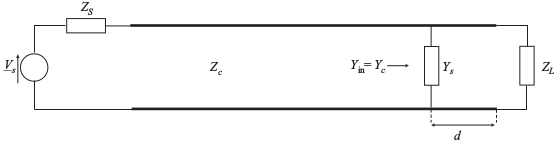
\includegraphics[scale=0.45]{ch3/image12.png}
	\captionof{figure}{ }
	\end{wrapfigure}				
	L'écart entre deux front d'onde est le même partout et vaut $\Delta z = 2\pi/k=\lambda$, la longueur d'onde et 
	ce peu importe où l'on se situe. Ce n'est "normal" que si on supprime la diffraction. Il faut remarquer 
	que le $\Delta z$ est pris parallèlement à l'axe $z$ alors que l'on considère la longueur d'onde 
	perpendiculairement au front d'onde, les deux situations sont différentes. Dans la lentille, on translate (rien 	    ne change entre 0 et $z$, pas de diffraction), alors que dans l'air le rayon de courbure devient de plus en plus petit (il y a en quelque sorte diffraction).\\

	Supposons que la variation du champ transverse incident se fait à une longueur caractéristique $\Delta l$. 
	On peut voir la lentille comme une fonction "fenêtre", limitant la taille du champ. C'est ce $\Delta l$ qui 
	va donner la valeur de $\rho$ pour étudier l'approximation. Pour se faire, regardons $A(\rho)$ la 
	transformée de Fourier de la fonction fenêtre, un sinc. La valeur maximal de $\rho$ vaut $\approx 2\pi/
	\Delta l$. Dans notre approximation
	\begin{equation}
	\frac{\rho^2}{2k}\Delta_0 \ll 1\qquad \Leftrightarrow\qquad \dfrac{4\pi^2\Delta_0}{2k\Delta l^2}\ll 1
	\end{equation}
	avec $k=2\pi/\lambda$ :
	\begin{equation}
	\Delta_0 \ll \dfrac{\Delta l^2}{\lambda}
	\end{equation}
	Il s'agit de l'inégalité inverse de celle de Fraunhofer : il fallait avoir une taille beaucoup plus grande 
	mais cette fois-ci comme la diffraction est négligée il faut être beaucoup plus petit.\\
	
	Pour exprimer la fonction de transfert, il faut exprimer la phase accumulée dans la lentille. Pour 
	un chemin optique $\Delta z$ parallèle à l'axe optique on peut facilement exprimer le déphasage. En effet 
	avec \autoref{eq:amod} 
	\begin{equation}
	\Delta\varphi = k\Delta z
	\end{equation}
	\begin{wrapfigure}[12]{l}{5.4cm}
	%\vspace{-5mm}
	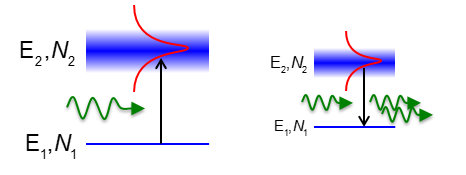
\includegraphics[scale=0.45]{ch3/image13.png}
	\captionof{figure}{ }
	\end{wrapfigure}		
	Dès lors, la phase accumulé dans la lentille vaudra simplement $\Delta \varphi(x,y) = k\Delta (x,y)$. 
	Comme on travaille sur la phase, il faut la définir pour une valeur de $z$ donnée (passage du plan 
	d'entrée au 	plan de sortie). Il faudra alors considérer la passage dans l'air, sans diffraction :
	\begin{equation}
	\Delta \varphi(x,y) = k\Delta (x,y) + k_0[\Delta_0-\Delta(x,y)]
	\end{equation}
	Il s'agit du déphasage introduit par la lentille en un point $(x,y)$ du plan transverse. Or, 
	$\Delta(x,y)$ est connu : à partir du champ dans le plan d'entrée $a(x,y)$ on pourra connaître le 
	champ $a'(x,y)$	dans le plan de sortie 
	\begin{equation}
	a'(x,y) = a(x,y)\underbrace{e^{i\Delta\varphi(x,y)}}_{T(x,y)}
	\end{equation}
	Le facteur de phase représente la phase accumulée du plan d'entrée au plan de sortie, y compris les 
	passages dans l'air. Attention, si la fonction de transfert ne contient que ceci, cela signifie que 
	que toute variation de l'amplitude du champ est négligée : l’absorption et les réflexions dans le 
	diélectrique sont négligées. Ceci définit la fonction de transfert $T(x,y)$.\\
	
	On peut écrire, en distribuant : $\Delta\varphi(x,y) = k_0\Delta_0 + (k-k_0)\Delta(x,y)$. Comme 
	$k=k_0n$, l'expression devient
	\begin{equation}
	\Delta\varphi(x,y) = k_0\left[\Delta_0+(n-1)\Delta(x,y)\right]
	\end{equation}
	En substituant l'expression de $\Delta(x,y)$ et après simplifications
	\begin{equation}
	\Delta \varphi(x,y) = k_0\left[n\Delta_0-(n-1)\dfrac{x^2+y^2}{2}\left(\dfrac{1}{R_1}+\dfrac{1}{R_2}\right)
	\right]
	\end{equation}
	Introduisons un nouveau paramètre
	\begin{equation}
	\frac{1}{f} \equiv (n-1)\left(\dfrac{1}{R_1}+\dfrac{1}{R_2}\right)
	\end{equation}
	afin d'écrire
	\begin{equation}
	\Delta\varphi(x,y) = k_0\left[n\Delta_0 - \dfrac{x^2+y^2}{2f}\right]
	\end{equation}
	Notre fonction de transfert devient alors
	\begin{equation}
	T(x,y) = e^{ik_0 n\Delta_0}\ e^{-i\frac{k_0}{2f}(x^2+y^2)}
	\end{equation}
	Le premier terme, de phase constante, revient à changer l'origine : on n'en tiendra pas compte ici (pas 
	d'interprétation physique si l'on n'étudie pas la dynamique de passage dans la lentille).
	En effet,
	
	\begin{equation}
	b(x,y)= a(x,y) e^{-i\omega_0 t} \Rightarrow b(x,y) = a(x,y) e^{-i\dfrac{k}{2f}(x^2+y^2)} \underbrace{e^{ik_0\Delta_0 n -i\omega_0t}}_{e^{-i\omega_0\left[t-\dfrac{k_0\Delta_0 n}{\omega_0}\right]}}
	\end{equation}
	
	On ne garde 
	que le terme de phase quadratique, ce qui est normal vu notre approximation parabolique. 
	\begin{equation}
	T(x,y) =\DS e^{\DS -i\frac{k_0}{2f}(x^2+y^2)}
	\end{equation}
	On verra que $f$ n'est autre que la \textit{distance focale} de la lentille (qui ne contient que l'indice de 
	réfraction et les rayons de courbures).

\newpage
\section{Fonction de transfert : interprétation}	
	\begin{wrapfigure}[10]{l}{7.4cm}
	\vspace{-5mm}
	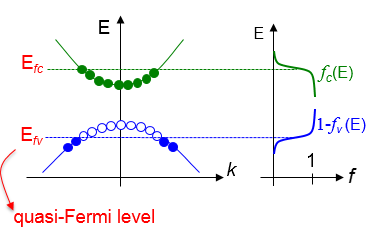
\includegraphics[scale=0.45]{ch3/image14.png}
	\captionof{figure}{ }
	\end{wrapfigure}		
Il est maintenant temps de faire l'interprétation physique de cette fonction. Le paramètre $f$ est défini 
par 
\begin{equation}
\frac{1}{f} \equiv (n-1)\left(\dfrac{1}{R_1}+\dfrac{1}{R_2}\right)
\end{equation}
L'indice de réfraction contient toute l'information du diélectrique, il est donc logique de le voir 
apparaître ici. On trouve également des paramètres géométriques.  Dans l'approximation des lentilles 
minces ($\Delta_0\ll R_1,R_2$ afin de négliger la diffraction entre le plan d'entrée et de sortie), nous 
avions obtenu
\begin{equation}
a'(x,y) = a(x,y)e^{-i\dfrac{k_0}{2f}(x^2+y^2)}
\end{equation}
Le terme de phase constant représentant la propagation dans la lentille a été négligé, celui-ci ne 
représentait qu'une modification de l'origine. \\

Dans le cadre de la description des lentilles minces, une lentille a une épaisseur dite "nulle" : on 
passe du plan $z=0^-$ au plan $z=0^+$. Cela permet de justifier le fait que l'on a omis le facteur de 
phase constante. \\

	\begin{wrapfigure}[12]{l}{8.4cm}
	\vspace{-5mm}
	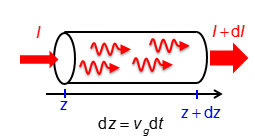
\includegraphics[scale=0.45]{ch3/image15.png}
	\captionof{figure}{ }
	\end{wrapfigure}		
Ce rappel étant fait, passons à l'interprétation. Considérons l'incidence d'une onde plane se propageant 
parallèlement à l'axe $z$ : une onde plane étant caractérisée par $a_0e^{ikz}$, évaluée en $z=0^-$ cela 
donne $a(x,y)=a_0$ comme suggérer ci-dessous :
\begin{equation}
a(x,y) = a_0 a'(x,y) = a_0e^{-i\dfrac{k_0}{2f}(x^2+y^2)}
\end{equation}
La distribution de phase dans le plan de sortie est donnée par la phase de la fonction de transfert. 
Étudions-la, que représente-t-elle ? Recherchons des "fronts d'onde", c'est-à-dire les lieux de phases 
constantes valant un multiple de $2\pi$ les lieux des points sur lequel le champ est maximum

	\begin{wrapfigure}[12]{r}{4cm}
	\vspace{-5mm}
	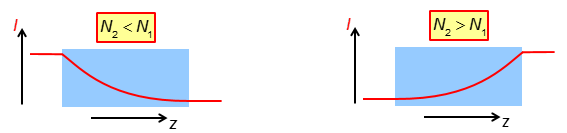
\includegraphics[scale=0.35]{ch3/image16.png}
	\captionof{figure}{ }
	\end{wrapfigure}	
\begin{equation}
\varphi = -\dfrac{k_0}{2f}\underbrace{(x^2+y^2)}_{R_m^2} = -2m\pi
\end{equation}

Le signe négatif est là pour la simplification. Représentons ce lieu des points dans le plan transverse, 
il s'agira bien entendu de cercles dont le rayon $R_m\propto \sqrt{m}$. On obtient ainsi l'interception
des fronts d'onde dans le plan de sortie.

\newpage
	\begin{wrapfigure}[8]{l}{4cm}
	%\vspace{-5mm}
	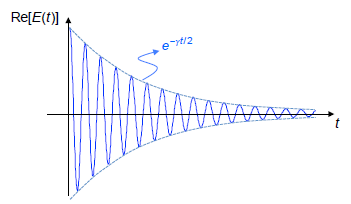
\includegraphics[scale=0.35]{ch3/image17.png}
	\captionof{figure}{ }
	\end{wrapfigure}	
Regardons maintenant ce que représente l'onde obtenue dans l'interception du plan de sortie. Pour se faire 
comparons la distribution de phase dans le plan $z=0^+$ à la distribution de phase d'une onde sphérique 
générée à un point $d$ de l'axe de la lentille. Dans le schéma ci-contre, $r$ est représenté jusqu'au plan 
de la lentille par facilité (et parce qu'on s'intéresse au plan de la lentille). Par Pythagore
\begin{equation}
r = \sqrt{d^2+x^2+y^2} \approx d + \dfrac{1}{2d}\left(x^2+y^2\right)
\end{equation}
La distribution de phase du champ de l'onde sphérique de l'onde dans le plan $z=0$ est alors donnée par
\begin{equation}
(x,y;0) \propto e^{ik_0d}\ e^{i\dfrac{k_0}{2d}(x^2+y^2)}
\end{equation}
Ceci ressemble à la distribution de phase obtenue à la sortie de la lentille. On peut également négliger 
le terme de phase constante. Une différence notable avec la sortie de la lentille est une différence de 
signe. Pour le comprendre, exprimons le champ avec sa dépendance temporelle
\begin{equation}
E(x,y,z,t) \propto e^{i(k_0r-\omega t)}
\end{equation}

	\begin{wrapfigure}[8]{r}{3.5cm}
	\vspace{-5mm}
	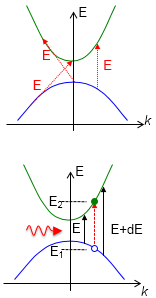
\includegraphics[scale=0.35]{ch3/image18.png}
	\captionof{figure}{ }
	\end{wrapfigure}
Les lieux de phases constantes en laissant filer le temps sont $\varphi = k_0 r-\omega t = c^{te}$. Lorsque 
le temps augmente, pour rester sur un front d'onde, il faut nécessairement que $r$ augmente pour compenser 
le signe négatif. Il s'agit d'une onde onde dont les rayons de courbure (le rayon $r$) augmente : onde 
sphérique divergente. En remplaçant un signe négatif dans notre onde sphérique l'onde sera bien convergente 
vers le \textit{foyer}. En effet, $\varphi = k_0 r+\omega t = c^{te}$, 
lorsque $t$ augmente, $r$ doit nécessairement diminuer \\

L'interprétation de la distribution de phase dans le plan de sortie n'est rien d'autre que la distribution 
de phase d'une onde convergente qui se focalise à la distance $f$ (si on remplace $d$ par $f$) 
la \textit{distance focale} de la lentille.\\

Une onde plane incidente sur la lentille donne une onde convergente au point focal $f$. Pour faire les 
choses plus rigoureusement, on peut appliquer la théorie de la diffraction pour montrer que la distribution 
de phase est bien celle d'une onde sphérique convergente. Prenons la formule de diffraction de Fresnel
\begin{equation}
a'(x,y,f) = \dfrac{k}{z}\iint a'(x',y';0^+) e^{i\frac{k}{2f}(x-x')^2}e^{i\frac{k}{2f}(y-y')^2}\ dx'dy'\ e^{ikf}
\end{equation}

	\begin{wrapfigure}[8]{l}{5.5cm}
	\vspace{-5mm}
	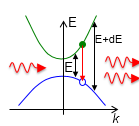
\includegraphics[scale=0.35]{ch3/image19.png}
	\captionof{figure}{ }
	\end{wrapfigure}
Il faut maintenant substituer l'expression de $a(x,y)$\footnote{Dans cette expression $k_0\rightarrow k$ car 
dans la théorie de Fresnel on travaillait déjà avec $k_0$ mais noté $k$.}. Pour simplifier, nous allons 
travailler à une seule dimension transverse
\begin{equation}
a'(x,f) = \sqrt{\dfrac{k}{f}}\int a'(x')e^{i\frac{k}{2f}(x-x')^2}\ dx'\ e^{ikf}
\end{equation}
La diffraction de ce champ jusqu'au point $f$ sera donné par application de la formule de Fresnel, ici à 
une dimension. 


\newpage
En substituant l'expression de $x'(x')$ 
\begin{equation}
a'(x,f) = \sqrt{\dfrac{k}{f}}\ a_0\int e^{\DS-i\frac{k}{2f}x^{'2}}\ e^{\DS i\frac{k}{2f}(x-x')^2}\ dx'\ e^{ikf}
\end{equation}
En effectuant le carré, l'expression se simplifie : le terme quadratique de phase en $x^{'2}$ se simplifie.
\begin{equation}
a'(x,f) = \sqrt{\dfrac{k}{f}}\ a_0\ e^{i\frac{k}{2f}x^2}\underbrace{\int  e^{\DS -i\frac{k}{f}xx'}\ dx}_{
\propto\ a_0\delta(x)}'\ e^{ikf}
\end{equation}
L'intégrale du facteur linéaire en $x'$ intégrée en $x'$ ne vaut zéro tant que le facteur avant le $x'$ 
n'est pas nul\footnote{?}, la seule valeur qui va en ressortir sera lorsque $x=0$. A la grosse louche, 
en deux dimension
\begin{equation}
a'(x,y;f) \propto\ a_0\delta(x,y)
\end{equation}
Le résultat de l'intégrale de Fresnel au point $f$ étant une delta de Dirac, l'onde se focalise au point 
$f$ : il s'agit bien d'une onde sphérique convergente.\\

	\begin{wrapfigure}[8]{l}{5.5cm}
	\vspace{-5mm}
	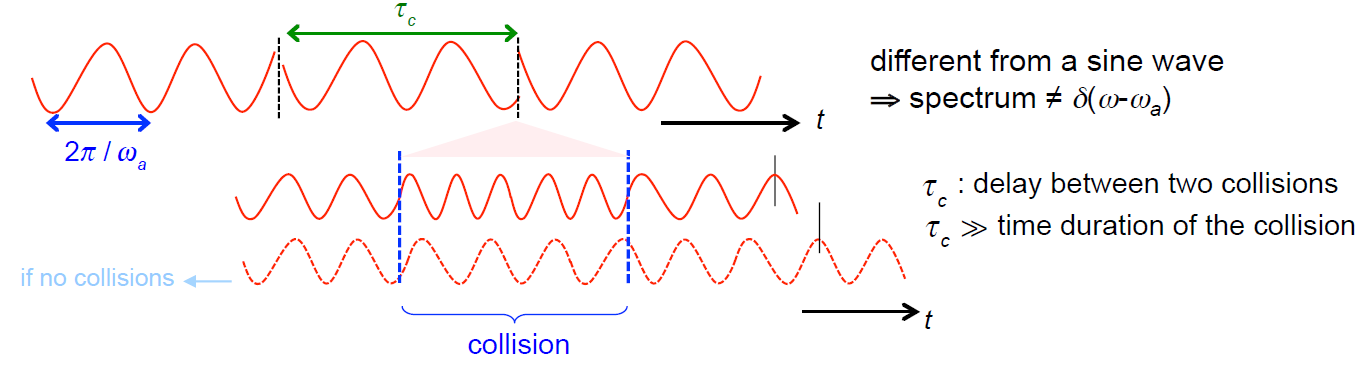
\includegraphics[scale=0.35]{ch3/image20.png}
	\captionof{figure}{ }
	\end{wrapfigure}
Généralisons en considérant une onde d'incidence oblique à l'aide du vecteur d'onde $\vec{k}$. Comme 
précédemment, le choix de $\rho_0$ fixe l'angle $\theta_0$. Dans le plan d'entrée de la lentille, on 
trouve
\begin{equation}
a(x,y) = a_0\ e^{i\rho_0x}
\end{equation} 
Ce qui multiplié par la fonction de transfert donne
\begin{equation}
a'(x,y) = a_0\ e^{i\rho_0x}\ e^{-i\dfrac{k}{2f}(x^2+y^2)}
\end{equation}
Étudions maintenant la diffraction de Fresnel (toujours à une dimension). En remplaçant le champ dans 
le plan incident et après simplification (comme précédemment) :
\begin{equation}
a'(x,f) = \sqrt{\frac{k}{f}}\ a_0\ e^{i\frac{k}{2f}x^2} \underbrace{\int e^{i\rho_0x'}\ e^{-i\frac{k}{f}xx'}\ dx'}_{
\propto\ a_0\delta(x-\frac{\rho_0f}{k} )} 
e^{ikf}
\end{equation}
Le résultat sera analogue au précédent : le champ transmis donne un pic d'intensité dans le plan focal de 
la lentille.
\begin{equation}
a'(x,y;f) \propto a_0\left(x-\dfrac{\rho_0f}{k},y\right)
\end{equation}

	\begin{wrapfigure}[8]{r}{7.5cm}
	\vspace{-5mm}
	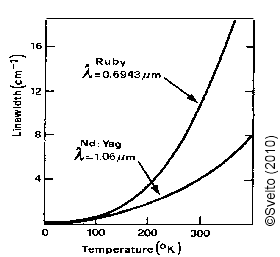
\includegraphics[scale=0.4]{ch3/image21.png}
	\captionof{figure}{ }
	\end{wrapfigure}
Le foyer ne se trouve plus sur l'axe focal mais bien dans le même plan que celui-ci : il s'agit du 
\textit{plan focal} et on parle de \textit{foyer secondaire}. A quoi correspond cette hauteur du 
point focal ? Sachant que $\rho_0/k = \sin\theta$ :
\begin{equation}
\dfrac{\rho_0f}{k} = f\sin\theta \approx f\theta_0 \approx f\tan\theta
\end{equation}
Ceci montre que la hauteur obtenue est la hauteur obtenue par la projection d'un rayon parallèle à $\vec{k}$, 
passant par le centre de la lentille, dans le plan focal. Cela permet d'établir la \textit{théorie des rayons}.\\

	\begin{wrapfigure}[9]{l}{5.5cm}
	\vspace{-5mm}
	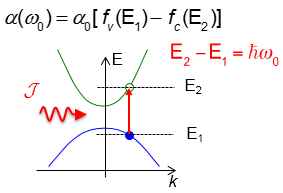
\includegraphics[scale=0.4]{ch3/image23.png}
	\captionof{figure}{ }
	\end{wrapfigure}
Les rayons sont ainsi des lignes partout perpendiculaires aux fronts d'onde (qui ne sera pas toujours 
droite). Ainsi, deux rayons parallèles devant la lentille se croisent dans le plan focal, au \textit{foyer secondaire}. 
Par réciprocité (revenons dans le temps), deux rayons émanant du point focal sont parallèles de l'autre côté de la 
lentille : on retrouve les règles de l'optique géométrique, tout est décrit dans la fonction de transfert.\\

Passons maintenant à l'interprétation physique de la fonction de transfert. Considérons n'importe quelle 
onde incidente sur la lentille. Solution des équations de Maxwell, on peut toujours la représenter comme
une somme d'onde planes (monochromatique, sans dépendance temporelle)
\begin{equation}
a(x;z) = \int A(\rho)e^{i\rho x}e^{i\sqrt{k^2-\rho^2}z}\ d\rho
\end{equation}
Tout onde peut être exprimée comme une somme d'onde plane, d'où l'importance de la précédente analyse : 
le principe de superposition va nous être précieux. Évalué dans le plan d'entrée de la lentille 
\begin{equation}
a(x;0) = \int A(\rho)e^{i\rho x}\ d\rho
\end{equation}
Commençons par regarder un terme de cette somme. Si l'on regarde le cas précédemment traité, nous 
avions $a(x) = a_0 e^{i\rho_0x}$. La différence est le changement suivant : $a_0\rightarrow A(\rho)d\rho$.
En substituant dans l'expression précédemment obtenue pour $a'(x;f)$ :
\begin{equation}
a'(x;f) \propto\ A(\rho)\delta\left(x-\frac{\rho f}{k}\right)\ d\rho
\end{equation}

	\begin{wrapfigure}[10]{r}{5cm}
	\vspace{-5mm}
	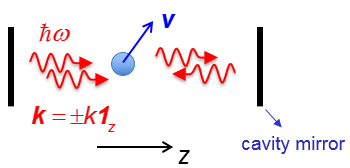
\includegraphics[scale=0.4]{ch3/image22.png}
	\captionof{figure}{ }
	\end{wrapfigure}
Ce qui a été fait pour une onde plane est vrai pour toute onde plane et par la principe de superposition, 
nous pouvons sommer le résultat. 

\begin{equation}
a'(x;f) \propto\ \int A(\rho)\delta\left(x-\frac{\rho f}{k}\right)\ d\rho
\end{equation}
On obtient le spectre multiplié par une delta de Dirac. En appliquant la Dirac
\begin{equation}
a'(x;f) \propto A\left(\dfrac{kx}{f}\right)
\end{equation}
La distribution à la sortie est donnée par le spectre du champ incident pour la variable $\rho$ devenue 
$kx/f$, la variable de Fourier est devenue une variable spatiale.\\

Pour l'interpréter, imaginons que l'on place un plan transparent sur le plan optique. Si l'on regarde 
le point $x_0$, celui-ci est le point focale d'une onde sphérique : on "sélectionne" une onde plane 
d'angle $\theta_0 = x_0/f$. On observe ainsi l'amplitude d'une onde d'angle $x_0/f$. Or, chaque valeur 
de $\theta$ correspond à une valeur de $\rho \longrightarrow \rho_0 = k\dfrac{x_0}{f}$.\\

Tout est cohérent, le $x_0$ sélectionne un $\rho_0$. A une hauteur $x$ donnée on retrouve bien 
l'amplitude du champ conditionnée à la hauteur où l'on regarde. 


\newpage
\section{Les lentilles et transformée de Fourier}
Une lentille effectue la TF du champ qui lui est incident, le but est d'ici de voir ça de façon 
plus rigoureuse. Avant ça, interprétons physiquement notre dernier résultat, à savoir
%	\begin{wrapfigure}[12]{l}{9.7cm}
%	\vspace{-5mm}
%	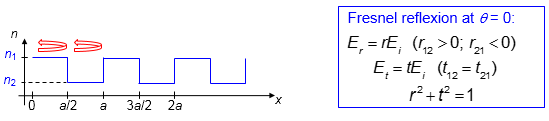
\includegraphics[scale=0.45]{ch3/image24.png}
%	\captionof{figure}{ }
%	\end{wrapfigure}		
\begin{equation}
a'(x,f)\propto A\left(\frac{kx}{f}\right)
\end{equation}
Pourquoi une lentille effectue-t-elle dans son plan focal la transformée de Fourier du plan qui 
lui est incident ? On peut voir le champ incident comme une superposition d'onde plane
\begin{equation}
a(x;z) = \int A(\rho)e^{i\rho x}e^{i\sqrt{k^2-\rho^2}z}\ d\rho
\end{equation}
où l'on reconnaît le spectre en $z=0$ (le propagateur tombe).  Considérons une des composantes de 
cette somme, à savoir une onde plane pour une valeur $\rho$. Celle-ci se transforme en onde 
sphérique pour se focaliser dans le plan focal en un foyer (ici secondaire) $x=\frac{\rho f}{k}$. 
On le sait car on peut dire que cette valeur de $x$ sélectionne une onde plane avec une certaine 
valeur de $\rho$, c'est-à-dire un angle $\theta$. L'amplitude de la delta de Dirac au point de 
focalisation vaut alors $A(\rho)$. Le $\rho$ dans $A(\rho)$ doit être traduit en terme de distribution 
dans le plan d'observation : il faut le décrire par rapport à la variable $x$. En isolant $\rho$ 
dans l'expression de $x$ on trouve
\begin{equation}
\rho = \dfrac{kx}{f}
\end{equation}
où $x/f = \tan\theta \approx \theta$. En ré-écrivant $A(\rho)$, on a bien le spectre en $kx/f$ :
\begin{equation}
A(\rho)\qquad\Longrightarrow\qquad A\left(\frac{kx}{f}\right)
\end{equation}
Nous ne connaissons qu'un facteur de proportionnalité, on peut s'attendre à trouver une distorsion 
de phase : le champ obtenu dans le plan focal contient la transformée de Fourier mais pas seulement.\\


	\begin{wrapfigure}[10]{l}{6.5cm}
	\vspace{-5mm}
	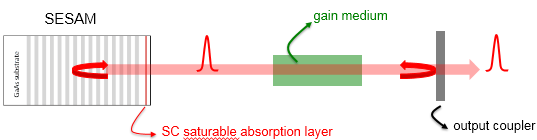
\includegraphics[scale=0.5]{ch3/image25.png}
	\captionof{figure}{ }
	\end{wrapfigure}		
Considérons un champ incident quelconque et étudions le champ dans un plan. Nous connaissons 
la fonction de transfert de la lentille
\begin{equation}
T(x,y) = e^{-i\frac{k}{2f}(x^2+y^2)}
\end{equation}
mais également la diffraction de Fresnel. La fonction de transfert nous informera ce qui se passe 
entre le plan entrant $a(x,y;0^-)$ et sortant $a(x,y;0^+)$ :
\begin{equation}
a(x,y;0^+) = a(x,y;0^-)e^{-i\frac{k}{2f}(x^2+y^2)}
\end{equation}
Fresnel nous donne la propagation du champ entre $z=0^+$ jusqu'au plan $z=f$ avec sa fameuse formule 
de diffraction:
\begin{equation}
a(x,y;z) = \frac{k}{z}\int a(x',y';0)\ e^{i\dfrac{k}{2z}(x-x')^2}\
 e^{i\dfrac{k}{2z}(y-y')^2}\ dx'dy'\  e^{ikz}
\end{equation}
Nous obtenons alors
\begin{equation}
a(x,y;f) = \dfrac{k}{f}\int a(x,y;0^-)e^{-i\frac{k}{2f}(x^{'2}+y^{'2})}\ e^{i\dfrac{k}{2z}(x-x')^2}\
 e^{i\dfrac{k}{2z}(y-y')^2}\ dx'dy'\  e^{ikf}
\end{equation}
Sachant que $(x-x')^2 = (x^2-2xx'+x^{'2})$ et de même pour le terme en $y$, on peut finalement 
obtenir (le facteur en $x^2$ et $y^2$ peuvent sortir de l'intégrale)
\begin{equation}
a(x,y;f) = \dfrac{k}{f}e^{i\frac{k}{2f}(x^2+y^2)}\int a(x,y;0^-)e^{-i\frac{k}{f}xx'}\ e^{-i\frac{k}{f}yy'}\  
dx'dy'\  e^{ikf}
\end{equation}
Il s'agit d'une intégrale avec des facteurs de phases linéaires. On peut faire apparaître la définition de 
la transformée de Fourier d'un champ
\begin{equation}
A(\rho, \sigma) = \int a(x',y',0)e^{-i\rho x'}e^{-i\sigma x'}\ dx'\ dy'
\end{equation}
Il nous suffit d'identifier : $\rho = kx/f$ et $\sigma = ky/f$.
\begin{equation}
a(x,y;f) = \dfrac{k}{f}e^{ikf} e^{i\frac{k}{2f}(x^2+y^2)}A\left(\frac{kx}{f},\frac{ky}{f}\right)  
\end{equation}
On voit que la lentille ne donne pas strictement une transformée de Fourier : celle-ci est multipliée 
par un facteur de phase quadratique.  Le résultat est quasi-identique à celui de Fraunhofer à une 
différence près : la distance de $z$ est finie et pas juste "suffisamment grande" comme c'était le cas 
pour Fraunhofer (nous avons ici juste fait l'approximation paraxiale).
\begin{equation}
a(x,y;z) = \dfrac{k}{z} e^{ikz} e^{i\dfrac{k}{2}(x^2+y^2)}\ A\left(\frac{kx}{z},\frac{ky}{z}\right)
\end{equation}
Nous allons faire l'analogie avec Fraunhofer. Si l'on n'observe que l'intensité (module carré du 
champ), la densité spectrale, celle-ci correspond bien à "seulement la transformée de Fourier". Comment 
interpréter ce facteur de phase additionnel ? \\

	\begin{wrapfigure}[8]{r}{5cm}
	\vspace{-8mm}
	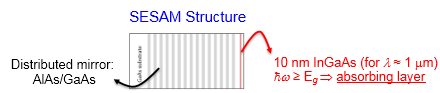
\includegraphics[scale=0.5]{ch3/image26.png}
	\captionof{figure}{ }
	\end{wrapfigure}		
Considérons comme champ incident une delta de Dirac centrée à l'origine, 
comme on néglige la diffraction dans la lentille, on aura une onde sphérique à la sortie de lentille :
ceci devrait générer une onde sphérique (de Huygens dans le cadre de Fraunhofer).
Ceci est totalement logique, le spectre de la 
fonction de Dirac est une constante :
\begin{equation}
A\left(\frac{kx}{f},\frac{ky}{f}\right)=1
\end{equation}
Dès lors
\begin{equation}
a(x,y;f) = \DS \dfrac{k}{f}e^{ikf} e^{i\frac{k}{2f}(x^2+y^2)}
\end{equation}

	\begin{wrapfigure}[9]{l}{5cm}
	\vspace{-12mm}
	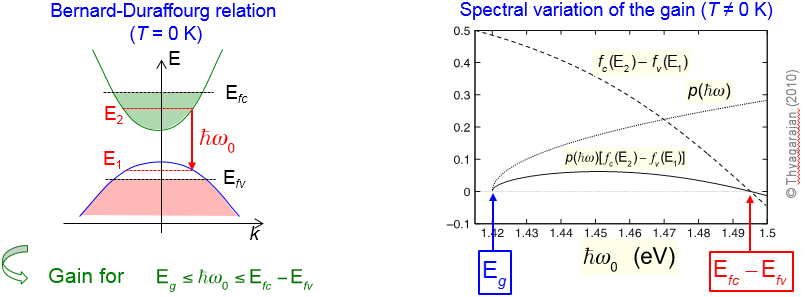
\includegraphics[scale=0.5]{ch3/image27.png}
	\captionof{figure}{ }
	\end{wrapfigure}	
Considérons cette fois un champ constant incident sur notre lentille. Celui-ci à une amplitude $a_0$ et 
une incidence nulle. Le spectre d'une constante étant une delta de Dirac, on obtient le résultat attendu
\begin{equation}
a'(x,y;z) = \frac{k}{f}e^{ikf}a_0\delta(x,y)
\end{equation}
Généralisons à toute distance  : on ne s'intéressant qu'au plan d'entrée, considérons maintenant une 
distance $d_0$ du plan d'entrée et on s'intéresse au champ dans le plan focal. Pour se faire, rappelons 
que le spectre $A(kx/f,ky/f)$ provient de la transformée de Fourier du champ en $z=0^-$. Comment faire 
apparaître le champ en $-d_0$ ? Utilisons Fresnel, mais de façon intelligente : le résultat étant donné 
en fonction du spectre en $z=0^-$, nous n'allons pas exprimer le spectre dans le domaine spatial (soit 
le point de départ de sa théorie) :
\begin{equation}
a(x,y;z) = \iint A(\rho,\sigma;0)e^{i\rho x}e^{i\sigma y} e^{-i\frac{\rho^2}{2k}z}
e^{-i\frac{\sigma^2}{2k}z}\ d\rho d\sigma\ e^{ikz}
\end{equation}

	\begin{wrapfigure}[10]{r}{8cm}
	\vspace{-2mm}
	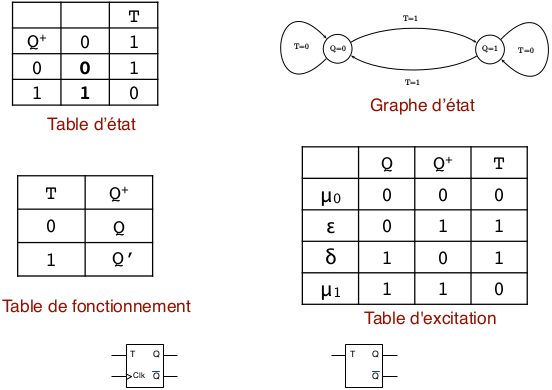
\includegraphics[scale=0.5]{ch3/image28.png}
	\captionof{figure}{ }
	\end{wrapfigure}	
Ceci dit qu'un champ peut être décomposé en onde plane où le propagateur s'est vu approximer par l'
approximation paraxiale. Ceci nous donne le champ en $z$ à partir du spectre en 0. Le propagateur 
apporte bien la diffraction. On y voit un nouveau spectre qui n'est plus $A(\rho,\sigma;0)$ mais
\begin{equation}
A(\rho,\sigma;z) = A(\rho,\sigma;0)e^{-i\frac{\rho^2}{2k}z}e^{-i\frac{\sigma^2}{2k}z} e^{ikz}
\end{equation}
Il s'agit de la \textit{propagation du spectre} : la multiplication du spectre par son propagateur 
donne le spectre à un autre endroit. Ceci montre donc comment se propage un spectre sur une distance 
$z$ (de 0 en $z$).  On peut utiliser cette expression pour une propagation sur une distance $d_0$ 
\begin{equation}
A(\rho,\sigma;0) = A(\rho,\sigma;-d_0)e^{i\frac{\rho^2}{2k}d_0-i\frac{\sigma^2}{2k}d_0} e^{ikd_0}
\end{equation}
En substituant $\rho$ et $\sigma$ :
\begin{equation}
A(\frac{kx}{f},\frac{ky}{f};0) = A(\frac{kx}{f},\frac{ky}{f};-d_0)e^{-\frac{i}{2k}\left(\frac{kx}{f}\right)^2d_0}e^{-
\frac{i}{2k}\left(\frac{ky}{f}\right)^2d_0} e^{ikd_0}
\end{equation}

	\begin{wrapfigure}[10]{l}{7cm}
	\vspace{-5mm}
	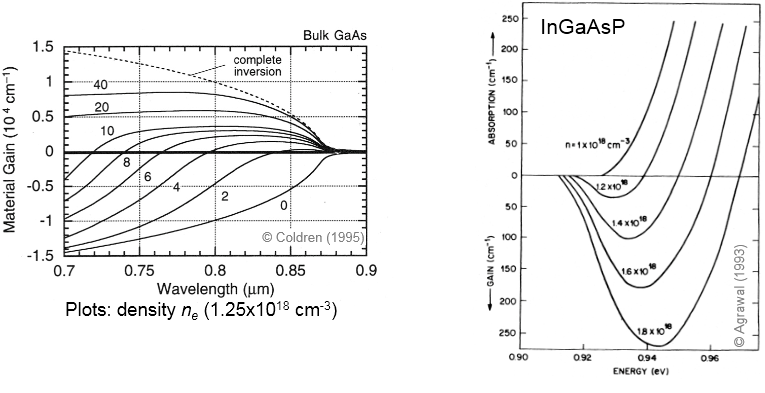
\includegraphics[scale=0.5]{ch3/image29.png}
	\captionof{figure}{ }
	\end{wrapfigure}
En simplifiant et en considérant une distance objet valant la distance focale $d_0=f$ :
\begin{equation}
A(\frac{kx}{f},\frac{ky}{f};0) = A(\frac{kx}{f},\frac{ky}{f};-f)e^{-\frac{k}{2f}x^2}e^{-\frac{k}{2f}y^2}
e^{ikf}
\end{equation}
En substituant ce résultat 
\begin{equation}
a(x,y;f) = \dfrac{k}{f}e^{ikf} e^{i\frac{k}{2f}(x^2+y^2)}A(\frac{kx}{f},\frac{ky}{f};-f)e^{-\frac{k}{2f}x^2}e^{-\frac{k}{2f}y^2}
e^{ikf}
\end{equation}
Les facteurs quadratiques se simplifie : il n'y a plus d'autres dépendances en $x,y$ que celles du 
spectre de l'onde
\begin{equation}
a(x,y;f) = \dfrac{k}{f}e^{2ikf} A\left(\frac{kx}{f},\frac{ky}{f};-f\right)
\end{equation}
Ceci montre que grâce à une lentille, on peut retrouver la transformée exacte d'un champ (on fait de 
l'optique qualitative, pas besoin des termes constant devant) si le champ est considéré à la distance 
focale $d_0=f$. 
\begin{equation}
a(x,y;f) \propto A\left(\frac{kx}{f},\frac{ky}{f};-f\right)
\end{equation}
Dans le plan focal image, nous aurons la transformée de Fourier \textbf{exacte} de ce champ pour un 
champ incident à $d_0=f$.








\chapter{La machine à courant continu}
Ces machines ne sont plus utilisées comme génératrices de puissances 
mais leurs capacité de réglage de vitesse nous pousse à les étudier. 
\textbf{Dynamo} est le nom donné à une génératrice à courant continu.

\section{Génération d'une tension continue}
	\subsection{Effet d'un collecteur}
	Pour avoir une f.e.m. continue, il faut 
	\begin{enumerate}
	\item Un collecteur
	\item Augmenter le nombre de conducteurs actifs
	\end{enumerate}
	Le \textbf{collecteur} est un commutateur ayant pour but de 
	redresser la f.e.m. alternative\footnote{"En électrotechnique, 
	un collecteur commutateur rotatif est un organe permettant de 
	créer 	une connexion électrique entre une partie fixe (stator) 
	et une 	partie tournante (rotor), avec une fonction de 
	commutation pendant la rotation. On trouve ce genre de 
	collecteur dans les machines à courant continu et les moteurs 
	électriques universels.".}.\\
	\begin{wrapfigure}[10]{l}{8.2cm}
	\vspace{-5mm}
	\includegraphics[scale=0.34]{ch4/image1.png}
	\captionof{figure}{ }
	\end{wrapfigure}
	\textbf{Petit plus (Source : Wikipedia) :} \textit{Ce collecteur 
	commutateur rotatif consiste en un anneau conducteur de l'électricité  
	sectionné en un nombre pair de parties 
	isolées entre elles, fixé avec une entretoise isolante sur l'axe de 
	la machine. La connexion électrique est créée entre les parties 
	conductrices et la partie fixée sur le stator (bornier), par une ou 
	plusieurs paires de balais positionnées respectivement à 180$\ ^\circ$. 
	On alimente en électricité le bobinage du rotor par ces contacts 
	(fonctionnement en moteur) ou au contraire on récupère l'électricité 
	produite par le bobinage du rotor (fonctionnement en générateur).}\ \\
	
	L'idée de l'espacement de $\pi$ est que le sens du courant dans 
	l'anneau conducteur va s'inverser, permettant au rotor de continuer 
	à tourner comme on peut le voir sur l'illustration ci-contre.\\
	On obtiendra aux balais une f.e.m. unidirectionnelle et dans le circuit 
	extérieur un courant unidirectionnel. Cependant, la grandeur ce cette 
	f.e.m. et du courant qui en résulte ne sont pas constantes.
	
	\newpage
	\begin{wrapfigure}[11]{r}{6.8cm}
	\includegraphics[scale=0.4]{ch4/image2.png}
	\captionof{figure}{ }
	\end{wrapfigure}
	Considérons un exemple "réel". Cette machine est constituée de 
	\begin{itemize}
	\item[$\bullet$] Un inducteur, sur le stator possédant $p$ paires de 
	pôles saillants. La répartition de l'induction dans l'entrefer a une 
	forme trapézoïdale avec comme axe de symétrie l'axe \textit{longitudinal} 
	$d$. L'axe électriquement $\perp$ à celui-ci est l'axe \textit{transversal},
	$q$.
	\item[$\bullet$] 	Un induit, disposés sous la forme d'enroulements de 
	conducteurs placés dans les encoches du cylindre rotorique. On connecte 
	via les faces latérales du cylindre ces conducteurs pour former un 
	\textit{enroulement en tambour.} 
	\end{itemize}\ 
	
	Les conducteurs actifs réunis par ces liaisons sont situés sous les 
	pôles opposés, d’où il résulte une addition des f.e.m. induites.
	Le point médian de chaque conducteur est relié à une lame du collecteur. 
	La \textbf{commutation} d’une lame à l’autre se fait donc au moment 
	où un conducteur actif passe d’un pôle à l’autre. Il faut voir que la somme des 
	f.e.m est nulle dans toute la machine, ce n'est qu'au niveau des ballais où on 
	somme d'une part toutes les f.e.m positives et sur l'autre les négatives. Ces 
	groupes de conducteurs actifs sont appelé \textbf{dérivations}.
	
	
	\subsection{Machine multipolaire}
	\begin{wrapfigure}[8]{l}{4.5cm}
	\vspace{-5mm}
	\includegraphics[scale=0.3]{ch4/image2p.png}
	\captionof{figure}{ }
	\end{wrapfigure}
	On considérait jusqu'ici des machines à deux pôles inducteurs, soyons 
	fous et plaçons-en maintenant quatre. Par symétries, les f.e.m. seront 
	égales en grandeurs puisqu'on somme une tension soit positive soit négative 
	entre deux ballais\footnote{Enes se représente la situation du sens des courants en utilisant $q\vec{v}\times \vec{B}$ qui donne des courants entrant aux pôles N et des courants sortant aux pôles S. Sachant que $v = \frac{d\phi}{dt} = \frac{d}{dt}\int \vec{B} \vec{dS}$ et que la convention d'Haelterman disait que le $\vec{dS}$ est donné par la règle de la main droite quand on tourne avec le courant, on peut voir que le produit scalaire de B et dS est positif avant les ballais + et négatif avant les ballais -. C'est comme ça qu'il expliquerai la sélection des ballais positif et négatif.}. Si l'on connecte les balais opposés entre eux (
	les deux négatifs ensemble, de même pour les positifs) on obtient une 
	dynamo multipolaire à \textit{enroulement parallèles}. \\\\\\
	
	\subsection{Types d'enroulement d'induit}
	Problème complexe non abordé ici. Sachez juste que pour l'enroulement 
	en tambour, on peut avoir l'enroulement \textit{imbriqué} ou l'
	enroulement \textit{ondulé}.
	
	\subsection{Tension à vide en régime statique}
	Soit un enroulement en tambour (l'armature, $a$) de $N_C$ conducteurs 
	répartis uniformément en deux couches. Le nombre de spires $N_S=N_C/2$. 
	On va supposer l'induit infiniment divisé de sorte à avoir une densité 
	linéique de spires $N_S/(2\pi R)$. On suppose un rotor lisse.
	
		\subsubsection{Méthode des champs}
		\begin{wrapfigure}[11]{l}{4.8cm}
		\vspace{-5mm}
		\includegraphics[scale=0.4]{ch4/image3.png}
		\captionof{figure}{ }
		\end{wrapfigure}
		Soit une spire constituée d'un conducteur d'entrée 1 et de sortie 
		1'. Nous avons
		\begin{description}
		\item[$\beta_m$ :] la coordonnée angulaire mécanique de l'entrée 1
		\item[$\beta_m-\alpha_m$ :] la coordonnée mécanique de sortie 1'
		\end{description}				
		La f.e.m. engendrée dans la spire vaut (voir figure ci-contre pour 
		la convention de signe (conducteur entrant et sortant))
		\begin{equation}
		\begin{array}{ll}
		e_{spire} &= B(\beta_m)lv - B(\beta_m-\alpha_m)lv\\
		&= (B(\beta_m)-B(\beta_m-\alpha_m))lv
		\end{array}
		\end{equation}
		Si $\alpha_m = \pi/p$ la spire est \textit{diamétrale}. Le "sens" 
		du champ $B$ sera donc exactement opposé
		\begin{equation}
		\begin{array}{l}
		B(\beta_m-\alpha_m) = - B(\beta_m)\\
		\hookrightarrow e_{spire} = 2B(\beta_m)lv
		\end{array}
		\end{equation}
		Si $\alpha_m<\pi/p$ on parle de spire \textit{à pas raccourci} : 
		on définit 1" déphasé de $\pi/p$ en avant par rapport à 1' et 
		donc déphasé de $\delta_m = \pi/p-\alpha_m$ par rapport à 1. Par 
		symétrie\footnote{??}
		\begin{equation}
		 \begin{array}{ll}
		B(1') = -B(1")\qquad\text{ou}\qquad B(\beta_m-\alpha_m) &=-B(\beta_m
		-\alpha_m+\frac{\pi}{p})\\
		&=-B(\beta_m+\delta_m)		
		\end{array}
		\end{equation}
		Impliquant que $e_{spire} = e_1-e_{1'}=e_1+e_{1"}$, en considérant 
		$B>0$ sous la pôle nord.\\
		On peut alors avoir une répartition rectangulaire de l'induction
		\begin{center}
		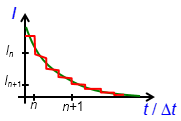
\includegraphics[scale=0.5]{ch4/image4}
		\end{center}
		ou  trapézoïdale 
		\begin{center}
		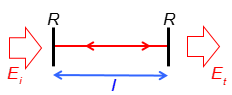
\includegraphics[scale=0.5]{ch4/image5}
		\end{center}
		
		\textsc{Forces électromotrice entre balais}\ \\
		\begin{wrapfigure}[12]{l}{6cm}
		\vspace{-2mm}
		\begin{equation}
		\begin{array}{ll}
		e &= \displaystyle p \int_{-\frac{\pi}{2p}}^{\frac{\pi}{2p}} 
		e_{spire}.\text{densité de spire}\\
		&= \displaystyle p \int_{-\frac{\pi}{2p}}^{\frac{\pi}{2p}} (
		2B(\beta_m)lv)\frac{N_s}{2d\pi}\ d\beta_m\\
		&= \displaystyle \frac{p}{d}N_s\frac{\Omega_r}{\pi} \int_{-
		\frac{\pi}{2p}}^{\frac{\pi}{2p}}B(\beta_m)lR\ d\beta_m\\
		&= \displaystyle\frac{p}{d}N_s\frac{\Omega_r}{\pi}\Phi
		\end{array}
		\end{equation}

		\end{wrapfigure}
		Supposons un enroulement à spires diamétrales tel que $e_{spire} = 
		2B(\beta_m)lv$. La f.e.m. entre balais est constante si l'induit 
		est infiniment divisé. Considérons un enroulement ondulé à $2d$ 
		dérivations : une dérivation comporte $N_S/(2d)$ spires. Celle-ci 
		est constitués par des spires dont les conducteurs d'entrée et 
		de sorties sont sous des pôles de même signe, il y a donc 
		$(N_S/2d).(1/\pi)$ spires appartenant à une dérivation par rad. 
		mécanique. Pour obtenir la tension aux bornes de la dérivation, 
		il faut intégrer les tensions de chaque spire de la dérivation. 
		Comme il y a $p$ paires de pôles, il convient de multiplier le 
		résultat d'un pôle par $p$. De façon générale :\\
		
		\retenir{\begin{equation}
		e = K\ \Omega_r\ \Phi
		\label{eq:4.5}
		\end{equation}
		où	$\Phi$ est le flux utile (coupé par une spire diamétrale 
		d'axe longitudinal de l'induit) par pôle, $\Omega_r$ en rad/s et 
		$K$, une constante qui dépend des données de l'enroulement.}\ \\

		\begin{wrapfigure}[12]{l}{4.8cm}
		\includegraphics[scale=0.4]{ch4/image6.png}
		\captionof{figure}{ }
		\end{wrapfigure}
		La f.e.m. (tension à vide) d'une dynamo est $\propto$ au flux 
		utile par les pôles et la vitesse de rotation. Cette formule 
		reste valable pour une machine en charge ($i_a\neq0$) si on 
		considère que $\Phi$ pourrait être modifié par $i_a$. $\Phi$ 
		dépend de $i_e$ de façon non-linéaire (cf. labo).\\
		
		Ci-contre, la répartition des f.e.m. engendré pour une dynamo 
		à induit infiniment divisé de spires diamétrales. La tension 
		entre deux balais est la somme ($\int$) de toutes les f.e.m. 
		sous un même pôle. Ce schéma confirme que la f.e.m. est bien 
		alternative mais constante en un point fixe : 
		\textbf{pseudo-stationnaire} du à l'effet redresseur du 
		collecteur.

		\subsubsection{Méthode des circuits}
		\begin{wrapfigure}[10]{r}{2.8cm}
		\vspace{-5mm}
		\includegraphics[scale=0.5]{ch4/image7.png}
		\captionof{figure}{ }
		\end{wrapfigure}
		Soit deux enroulements : un d'excitation parcouru par $i_e$ 
		et un induit pseudo-stationnaire à vide. A bornes du balais, 
		on a donc
		\begin{equation}
		v_a = R_ai_a+D\Psi_a
		\end{equation}
		où $\Psi_a$ est le flux coupé par l'enroulement induit, flux 
		créé par le courant d'excitation. On peut écrire
		\begin{equation}
		\Psi_a = M(\beta_m,i_e)i_e
		\end{equation}
		où $M$ est l'inductance mutuelle entre les enroulement $e$ 
		et $a$, mutuelle fonction de $\beta$, l'angle de décalage 
		entre $N$ et l'axe d'enroulement. En faisant les math ;
		\begin{equation}
		\begin{array}{ll}
		(v_a)_{i_a=0} &= \displaystyle D\Psi_a\\
		&= \displaystyle D(Mi_e)\\
		&= \displaystyle  DM\ i_e + M\ Di_e\\
		&= \displaystyle \frac{\partial M}{\partial \beta_m}D\beta_m
		i_e + \frac{\partial M}{\partial i_e}Di_e i_e + M\ Di_e\\
		&= \displaystyle G(\beta_m,i_e)\Sigma_r i_e +\left(M+\frac{
		\partial M}{\partial i_e}i_e\right)Di_e
		\end{array}
		\end{equation}
		On définit alors la valeur locale (ou différentielle) de la 
		mutuelle : $\displaystyle M' = M+\frac{\partial M}{\partial 
		i_e}i_e$, qui sera nulle si les balais sont calés sur l'axe 
		neutre ($\beta = \pi/2$) car $a \perp e$. \\
		On définit également la \textbf{fonction d'excitation}
		\begin{equation}
		G(i_e) = \frac{\partial M(\beta_m,i_e)}{\partial \beta_m}) =
		\frac{(\partial \Psi_a/\partial \beta_m)}{i_e}\qquad si\qquad 
		\beta=\frac{\pi}{2}, i_e=\text{ cste}
		\end{equation}
		La f.e.m. vaut alors $e = (v_a)_{i_a=0} = G(i_e)i_e\Omega_r$ 
		qui ressemble à notre belle formule encadré plus haut ! On 
		peut dès lors écrire
		\begin{equation}
		G(i_e)i_e = K\Phi
		\end{equation}
		La connaissance de la caractéristique à vide qui conduisait 
		immédiatement à la détermination de $K, \Phi$ en fonction de 
		$i_e$, il en est de même pour $G$ en fonction de $i_e$.
		
	\subsection{Effet de décalage des balais}
	\begin{wrapfigure}[7]{r}{9.5cm}
	\vspace{-8mm}
	\includegraphics[scale=0.5]{ch4/image8.png}
	\captionof{figure}{ }
	\end{wrapfigure}
	Dans l'expression de la tension à vide, on a maintenant comme 
	limites $-\frac{\pi}{2}p+\gamma_m$ et $\frac{\pi}{2}p+\gamma_m$ (à 
	la place de $-\frac{\pi}{2}p+$ et $\frac{\pi}{2}p$), réduisant la 
	valeur de celle-ci par rapport à leurs positions sur les axes neutres. 
	Il faut encore rajouter à ça un effet de mutuelle.
	
	\subsection{Tension à vide - modèle mathématique}
	Trois remarques sur ce qu'est un bon modèle
	\begin{enumerate}
	\item Adapté au but poursuivi, ça ne sert à rien de faire trop.
	\item Il doit être simple, sinon avoues que tu ne le liras pas.
	\item Il doit être homogène, si on applique une hypothèse il faut 
	toujours l'appliquer.
	\end{enumerate}\ \\
	
	\textsc{Exemple - dynamo à vide}\\
	Définissions comme variables de commande $v_e$ la tension aux bornes 
	du circuit d'excitation, $\Omega_r$ la vitesse de rotation et $e$, 
	la tension à vides aux bornes des balais comme variable de sortie. 
	Connaissant deux expressions pour $e$, il suffit d'en prendre une et 
	de la compléter par l'équation du circuit d'excitation pour obtenir le 
	modèle recherché : $v_e = R_ei_e +D\Psi_e$.
	
		\subsubsection{Modèle non-linéaire}
		Il suffit d'utiliser une relation non-linéaire entre $\Psi_e$ 
		et $i_e$ pour compliquer le tout : $\Psi_e = L_e(i_e)i_e$ où 
		$L_e$ est l'inductance propre du circuit d'excitation, fonction 
		non-linéaire. Si l'on considère que $\Psi_e$ est variable d'état :
		ré-écrivons notre équation sous la forme d'une ED :
		\begin{equation}
		D\Psi_e = v_e-R_ei_e(\Psi_e)
		\end{equation}
		Si cette fois on choisi $i_e$ comme variable d'état, on peut 
		écrire
		\begin{equation}
		\dfrac{\partial \Psi_e}{\partial i_e}Di_e = v_e-R_ei_e\quad 
		\Longrightarrow\quad Di_e = \dfrac{v_e - R_ei_e}{L_e'}
		\end{equation}
		où $L_e'(i_e)$ est la valeur différentielle de l'inductance 
		propre du circuit $e$. Notons qu'elle est aussi égale à 
		$L_e+(\partial L_e/\partial i_e)i_e = \partial\psi_e/\partial 
		i_e$. Sachant que $e = (v_a)_{i_a=0} = G(i_e)i_e\Omega_r$, le 
		calcul de $e$ est immédiat si l'on a $i_e$.\\

		\begin{wrapfigure}[6]{l}{7cm}
		\vspace{-8mm}
		\includegraphics[scale=0.5]{ch4/image9.png}
		\captionof{figure}{ }
		\end{wrapfigure}
		Nos deux équations trop stylées 
		\begin{equation}
		\begin{array}{ll}
		v_e &= R_ei_e + L_e Di_e\\
		e &= K\Phi\Omega_r = G\Omega_ri_e
		\end{array}
		\end{equation}
		nous fournissent un schéma équivalent dont la caractéristique 
		permet le passage de $\Psi_e$ à $i_e$.
		
		Il est également possible, via $D\Psi_e = v_e - R_ei_e(\Psi_e)$ 
		d'obtenir le schéma-bloc suivant :
		\begin{center}
		\includegraphics[scale=0.5]{ch4/image10.png}
		\captionof{figure}{ }		
		\end{center}			
		
		\subsubsection{Modèle linéaire}
		On peut l'obtenir en considérant de "petits mouvements" et en 
		substituant les courbes par leurs tangentes. Supposons que 
		$L_e = L_e' = L_{e,ns} = \text{cste}$ et $G = G_{ns} = 
		\text{cste}$. Notre précédente relation devient alors 
		\begin{equation}
		Di_e = \frac{v_e - R_ei_e}{L_e} \quad \lt\quad I_e(p) : 
		\frac{1}{1+pT_e}\frac{V_e(p)}{R_e}
		\end{equation}
		où $T_e = L_e/R_e$ est la constante de temps du circuit d'
		excitation (valeur assez élevée comme beaucoup d'enroulements). 
		Cette relation obtenue via Laplace est assez évidente à vue 
		du schéma équivalent, car ce-dernier est constitué de $R_e$ 
		et $L_e$. La grandeur de sortie vaut toujours 
		\begin{equation}
		e = Gi_e\Omega_r
		\end{equation}
		et dépend linéairement de $i_e$ si la vitesse est constante. 
		Le système global est du premier ordre
		\begin{equation}
		E(p) = G\Omega_r I_e(p) = G\Omega_r \dfrac{1}{1+pT_e}\frac{V_e
		}{R_e}
		\end{equation}
		\begin{center}
		\includegraphics[scale=0.5]{ch4/image11.png}
		\captionof{figure}{ }		
		\end{center}			
		
			
\section{Influence du courant d'armature}
En effet, ça on sent que la machine en charge comportera en plus d'une 
source de tension une résistance $R_a$ et une inductance $L_a$.

	\subsection{Effet Joule (résistance $R_a$)}
	On les trouve dans l'enroulement ainsi que dans le ballais/collecteur,
	dépendant de plusieurs paramètres tel que la température et la valeur du courant.
	Mesurer la résistance globale n'est pas aisé, la résistance n'étant 
	pas la même quand la machine est en fonction ou non : en rotation, 
	elle est perturbée par la f.e.m. rémanente. En gros, les chutes sont 
	\begin{equation}
	\Delta V_{R_a} = \Delta V_b\text{sign}(i_a) + R_ai_a
	\end{equation}
	où $\Delta V_b$ représente la chute balais collecteur (fonction du 
	sens de rotation) et $R_a$ la résistance entre enroulements. Par 
	\textbf{convention}, la chute est fixée à $2V$ pour les balais en 
	carbone et $0.6V$ pour les métalliques.
	
	\subsection{Réaction transversale de l'armature infiniment divisée}
	\begin{wrapfigure}[9]{l}{4.7cm}
	\vspace{-5mm}
	\includegraphics[scale=0.34]{ch4/image12.png}
	\captionof{figure}{ }
	\end{wrapfigure}
	Soit une génératrice avec un courant infiniment divisé qui circule 
	dans l'induit, même sens que la f.e.m. Les courants induits créent 
	à leurs tour un champ créant un flux perpendiculaire au flux 
	inducteur. En désignant $\beta_m$ l'abscisse angulaire d'un point, 
	calculons les ampères-tours dans un contour d'induction fermé :
	\begin{equation}
	\frac{N_c}{2\pi}\frac{i_a}{2d}2\beta_m
	\end{equation}
	Par symétrie par rapport à l'axe des pôles, la moitié des A.t. est 
	attribué à la moitié du chemin. Par abus, on attribue des A.t. la 
	ou le chemin traverse l'entrefer. Si ce dernier est constant et le 
	fer parfait 
	\begin{equation}
	H(\beta_m) = \frac{N_c}{2\pi}\frac{i_a}{2d}\frac{\beta_m}{\delta}
	\end{equation}
	$H$ est max si $\beta_m=\pi/2p$ : 
	\begin{equation}
	H\left(\frac{\pi}{2p}\right) = \frac{N_c}{2\pi}\frac{i_a}{2d}\frac{
	\pi}{2p\delta} = \frac{N_c}{8\delta}\frac{i_a}{pd}=\frac{N_s}{4\delta}
	\frac{i_a}{pd}
	\end{equation}
	Si le fer est réel il suffit de multiplier par $\mu_0$. Tout ceci 
	est bien indépendant de la vitesse de rotation : la situation est 
	la même que si une bobine était alignée sur l'axe neutre.
	
		\begin{center}
		\includegraphics[scale=0.35]{ch4/image13.png}
		\captionof{figure}{ }		
		\end{center}
	
	Pour calculer $L_a$ on considère un enroulement fictif dont toutes 
	les spires ont par axe celui du balai : le flux vaudra l'intégrale 
	de l'induction entre $\beta_m et \pi-\beta_m$. Grâce au flux 
	totalisé : $L_a=\Psi_a/i_a$.
	
	\subsection{Le champ résultant}
		\subsubsection{Sans saturation}
		\begin{wrapfigure}[7]{r}{4.7cm}
	\vspace{-25mm}
	\includegraphics[scale=0.34]{ch4/image14.png}
	\captionof{figure}{ }
	\end{wrapfigure}
		On peut appliquer le principe de superposition. Pour une dynamo, 
		une fois la réaction d'induit est magnétisante (corne d'entrée) 
		et une fois démagnétisant (corde de sortie). La figure ci-contre 
		montre comment obtenir $B$ par la somme de l'induction de l'inducteur 
		$B_e$ et la réaction d'induit $B_a$.\\
		Notons que le flux par pôle n'a pas changé, la f.e.m. en charge est la 
		même qu'à vide. Cependant, l'induction est tantôt plus grande tantôt plus 
		faible par endroit, donc certaines spires supportent plus de tensions et il y a 
		risque de claquage entre les lames du collecteur. 
		
		\subsubsection{Avec saturation}
		L'induction en charge est plus petite que la somme de l'excitation 
		et la réaction d'induit. Le flux longitudinal est plus faible, 
		causant une f.e.m. plus faible $\rightarrow$\textit{ La réaction 
		d'induit possède une composante longitudinale à cause de la 
		saturation.}. Pour décrire l'effet démagnétisant, trois hypothèses :
		\begin{enumerate}
		\item Lignes de forces radiales dans l'entrefer.
		\item L'induction null en dehors des pôles.
		\item Démonstration faite pour $p=d=1$.
		\end{enumerate}
		A vide, juste avec le courant d'excitation $i_e$ on a $A.t._e = 
		N_ei_e$. Si la spire n'est pas sous le pôle sa tension est nulle. 
		Si par contre elle est sous le pôle elle sera $\propto B_e$. La 
		courbe a vide donne le lien entre $e$ et $N_ei_e$ mais aussi la 
		f.e.m. à une constante près.\\
		Les courants induits causent également des A.t. de réactions 
		d'induits qui varient linéairement entre la corne de sortie $-A$ 
		et d'entrée $+A$ de la sorte :
		\begin{equation}
		A = \frac{N_c}{2\pi}\frac{i_a}{2}\frac{b_i}{4\pi R}
		\end{equation}
		Les A.t. varient ainsi linéairement de $N_ei_e-A$ à $N_ei_e+A$ (
		$OP_1$ à $OP_2$ sur le schéma page 4.33). \textbf{Lire le texte 
		sur cette page, c'est assez confus. Enes confirme.}
		
		\subsection{Couple électromécanique - Couple extérieur}
		La loi de Laplace ($F+ilB$) permet de calculer la somme sur 
		chaque conducteur pour ensuite les sommer, mais il est plus 
		simple d'utiliser la conservation de la puissance : la somme 
		de la puissance appliquée électriquement et de la puissance 
		appliquée mécaniquement est nulle\footnote{? (en convention 
		récepteur)} :
		\begin{equation}
		[\underbrace{P_{electrique} - (P_{pJoule}}_{P_{electromecanique}}
		+P_{pmagn})] + [P_{mecan}-P_{meca}]=0
		\end{equation}
		où les pertes joules $P_{pJ}=0$ si $î_a=0$. Par contre les pertes 
		magnétiques existent tout de même (hystérèse, Foucault, ...). Les 
		pertes méca sont dues aux frottement (fonction de $\Omega_r$). La 
		puissance mécanique appliquée à un moteur est négative. On peut 
		calculer le couple électromécanique $P_{em} = C_{em}\Omega_r$. D'autre part,
		\begin{equation}
		\begin{aligned}
			P_{em} &= P_{électrique} - P_{pJ}\\
						 &= v_a i_a - \Delta V_b i_a -R_a i_a^2\\
						 &= e i_a
		\end{aligned}
		\end{equation}
		En utilisant \autoref{eq:4.5}, on trouve que 
		\begin{equation}
			C_{em} = K\Phi i_a = Gi_ei_a.
		\end{equation}
		En moteur, la réaction d'induit change de signe : magnétisante sous la corne polaire d'entrée.\\
		
		\textbf{Réécriture de Nicolas Englebert}
		
	\subsection{Inconvénients de la réaction d'induit}
	Cette réaction cause trois effets néfastes :
	\begin{enumerate}
	\item Déplacement de la ligne neutre ($B=0$) gênant la commutation
	\item Augmente l'indiction : risque de claquage entre les lames
	\item Cause de l'inductance du rotor, s’opposant aux variations rapides 
	du courant induit et donc du couple
	\end{enumerate}
	
	
	\subsection{La commutation}
	La commutation concerne tous les phénomènes inversant le signe du courant 
	par court-circuit/circuit ouvert avec les balais. Comme il y a frottement, 
	il peut y avoir étincelles !
	
	\begin{description}
	\item[Causes mécaniques] Certaines lames bombées, vibrations, mauvais 
	équilibrage, \dots
	\item[Causes électriques] Théoriquement très compliqué
	\end{description}
	Détaillons légèrement ce point \textit{compliqué} avec la théorie de ARNOLD. 
	On se débarasse d'abord de toute imperfections mécaniques en trois hypothèses :
	état mécanique parfait, résistivité balais/collecteur constante, égalité de 
	la largeur d'un balai et d'une lame.\\
	
	Le souci est inductif. Au moment de la commutation, l'inductance à tendance 
	à ne pas laisser passer le courant. Plus mathématiquement, à cet instant la 
	dérivée du courant subit une discontinuité causant une surtension importante : 
	rupture de l’isolation et risque de claquage.\\
	
	Au cours oral, le prof a dit qu'il ne poserait pas de question de démonstration sur cette partie. Lire et comprendre le phénomène au travers les équations peut s'avérer utile. \\
	
	\textsc{Le remède de grand-mère}.\\
	L'idée est de créer un phénomène d'amplitude 
	contraire et même encore plus fort (pour être sûr) pour contrecarrer cet 
	effet. On crée alors une fem opposée, favorable à la variation de courant afin 
	de permettre la variation de courant en fin de commutation. On crée cette fem 
	grâce a un flux d'axe neutre (transversal) au sens opposé à la réaction d'induit. On a dès lors l'intégration de pôles de commutation avec des enroulements de compensation. \\
	On pourrait aussi se dire \textit{"Pourquoi ne pas prendre un entrefer plus grand?"} 
	Effectivement, l'inductance diminue mais le flux d'excitation également ce qui 
	est moins avantageux. 
		

\section{Étude de la dynamique des machines}
	\subsection{Modèles mathématiques - schémas équivalents}
		\begin{wrapfigure}[10]{l}{8.7cm}
	%\vspace{-25mm}
	\includegraphics[scale=0.34]{ch4/image15.png}
	\captionof{figure}{ }
	\end{wrapfigure}
	Reprenons ce qui a été vu précédemment et synthétisons le sur le schéma ci-contre. 
	On va supposer que le modèle magnétique, les pertes, \dots sont linéaires. On 
	trouve 
	\begin{description}
	\item[$R_e$;] Résistance du circuit inducteur
	\item[$L_e$;] Inductance du circuit inducteur
	\item[$R_a$;] Résistance du circuit d'induit
	\item[$\Delta V_b$;] Chute de tension du contact balais-collecteur
	\item[$L_a$;] Inductance du circuit d'induit
	\item[$e$;] Force électromotrice engendrée $= Gi_e\Omega_r$
\end{description}		
	Notre tension d'excitation $V_e$ pourra être éventuellement réglable : $V_x$. La 
	zone en pointillé représente la machine, tandis que la partie de droite représente 
	le rotor, possédant une fem $e$ du à sa rotation.\\
	
	Lors de l'allumage, il faut fournir énormément de flux. Pour limiter ce courant, on 
	introduit des réhostas :
	\begin{description}
	\item[$R_d$ : rhéostat de démarrage;]  Sert à limiter le courant à la mise sous tension 
	$V_{al}$ car à vitesse nulle, $e=0$ et le courant est juste limité par $R_a$ et $L_a$ 
	de faible valeur.
	\item[$R_{exc}$ : rhéostat d'excitation;] Règle le courant d'excitation $i_e$ pour une 
	tension d'excitation $v_x$ donnée.
	\end{description}
	Les équations de ce modèles sont, pour rappel :
	\begin{equation}
	\begin{array}{ll}
	v_x &= (R_e+R_{exc}-i_e + L_e\frac{di_e}{dt}\\
	v_{al} &= e+\Delta V_b + (R_a+R_d)i_a + L_a\frac{di_a}{dt}\\
	e &= k\phi\Omega_r = Gi_e\Omega_r
	\end{array}
	\end{equation}
	Cette fois-ci, on doit ajouter l'équation de mouvement :
	\begin{equation}
	j\dfrac{d\Omega_r}{dt} = C_{em}+C_r
	\end{equation}
	avec $C_r$, le couple résistant du moteur (pertes magnétiques et mécanique). 
	Il doit être vu comme négatif, diminuant le couple appliqué par le moteur à l'arbre, 
	$C_{em}$.\\
	Il s'agit d'un modèle dynamique (dérivée). En laboratoire, tout peut être mis comme 
	étant constant. Sous la forme canonique, on obtient :
	\begin{equation}
	\begin{array}{ll}
	Di_e &= \frac{1}{L_e}[v_x-(R_e+R_{exc}i_e]\\
	Di_a &= \frac{1}{L_a}[v_{al} - \Delta V_b - Gi_e\Omega_r - (R_a+R_d)i_a]\\
	D\Omega_r &= \frac{1}{J}[Gi_ei_a - C_r(\Omega_r)]
	\end{array}
	\end{equation}
	Avec ces équations, il est facile d'obtenir le schéma bloc ci-dessous.  
	\begin{itemize}
	\item[$\bullet$] Notre sortie est bien la vitesse de rotation, définie par le couple 
	moteur.
	\item[$\bullet$] La première équation est représenté à gauche sur la branche $V_x$ : 
	on calcule $i_e$ à partir de $V_x$.
	\item[$\bullet$] La grandeur d'entrée de la deuxième équation est la tension d'alimentation. 
	Il faut ainsi partir de $V_{al}$, soustraire $Gi_e\Omega_r,\dots$. Le $Gi_e$ avait déjà été 
	calculé, $\Omega_r$ est à la sortie. Le rectangle central correspond ainsi à une partie de 
	cette deuxième équation
	\item[$\bullet$] Pour la troisième équation, nous avons $K\phi i_a$ et il faut rentrer 
	le couple résistant : on peut dire que le couple résistant dépend de la vitesse de 
	rotation
	\end{itemize}
	
	\begin{center}
	\includegraphics[scale=0.34]{ch4/image21.png}
	\captionof{figure}{ }
	\end{center}
	
	Supprimons la dernière rétroaction. Mettons notre pied sur l'intégrale pour avoir un couple 
	constant. Le couple moteur étant constant, la vitesse ne change pas directement (du à la grande 
	inertie)(nous 
	étions en situation de régime, on vient de briser cet équilibre). Mais maintenant, on sait que 
	la vitesse va diminuer. Sachant cela,  le carré avec (*) au milieu va être affecté. Comme 
	$i_e$ est contant, la fem $e$ va diminuer : déséquilibre le rond avec $\pm$.\\
	
	A l'examen oral, je peux négliger le bras tout en haut en affirmant que c'est un effet 
	correcteur pas très important, que l'ordinateur peut se charger de le calculer.\\
	
	Ceci étant dit, La valeur $V-e$ va commencer à être positive, le courant va alors 
	augmenter. Le couple moteur va alors lui aussi augmenter pour retrouver le couple appliqué 
	par mon pied et on retrouvera un nouveau point d'équilibre, avec une vitesse plus faible 
	mais un courant plus important (car couple plus important).\\
	
	Si la vitesse diminue de 1\%, la vitesse fait-elle de même ? Le courant augmentera en 
	réalité plus rapidement que cette diminution. Pour savoir à quel point, il faut annuler 
	toutes les dérivée pour se rendre compte que le terme $1/R_a$ est très important : le couple 
	va vite réagir à une petite variation.\\
	
	En faisant une analyse semblable, on peut voir que si on augmente $V_x$, le moteur va 
	tourner moins vite. L'augmentation de $V_d$ cause par contre une augmentation de la 
	vitesse.
	
	
\section{Courbes caractéristiques des génératrices}
	
	\subsection{Les différents types de génératrices}
	\begin{wrapfigure}[7]{l}{3cm}
	\vspace{-5mm}
	\includegraphics[scale=0.34]{ch4/image16.png}
	\captionof{figure}{ }
	\end{wrapfigure}
	On a toujours considéré que le courant d'excitation était fourni par une source 
	extérieure. Or, à cause du rémanent, une tension existe lors de la rotation entre 
	les balais de la machine pour un courant d'excitation nul. L'idée est d'utiliser 
	ce courant pour exciter la machine\footnote{Oh oui elle est chaude !}.\\
	S'il n'y a pas de charge, $i_e$ est très petit et on considère que la tension aux 
	bornes est la fem. Pour $\Omega_r$ donné, on a deux caractéristiques :
	\begin{enumerate}
	\item Caractéristique à vide $e = f(i_e)$.
	\item Loi d'Ohm du circuit d’excitation $e=(R_{exc}+R_e)i_e$.\footnote{En régime, 
	il n'y a que les résistances : la self se comporte comme un fil.}
	\end{enumerate}
	\begin{center}
	\includegraphics[scale=0.37]{ch4/image17.png}
	\captionof{figure}{ }
	\end{center}
	L'intersection donne le point de fonctionnement. On voit qu'il existe une valeur 
	de $R_{exc}$ au dela de laquelle la tension aux bornes est très faible (a). Si 
	on inverse les bornes, la machine ne s'amorce pas et si la machine est linéaire, 
	le seul point de fonctionnement est $e=0,i_e=0$ sauf si $R_{exc}+R_e=G\Omega_r$.\\
	
	En pratique, on rencontre trois types de génératrices :
	\begin{description}
	\item[Excitation dirigée / shunt] Beaucoup de spires pour avoir beaucoup 
	d'ampères-tours avec peu de flux
	\item[Excitation série] Ce type de moteur est caractérisé par le fait que 
	le stator (inducteur) est raccordé en série avec le rotor (induit) : le même 
	courant traverse le rotor et le stator. Cela offre une faible résistance, et 
	le nombre de spire nécessaire est moins important ($\approx 100$ fois moins qu'en 
	shunt).\footnote{ On fait tourner le moteur : entre les balais on obtient $e$. Pour avoir 
	le flux, on passe tout le courant dans l'excitation.}
	\item[Compoundage] Les deux en même temps.
	\end{description}
	
	
	\subsection{Caractéristiques à vide et en charge d'une machine à excitation 
	indépendante}
		\subsubsection{Fem à vide}
			\begin{wrapfigure}[7]{r}{3.3cm}
	\vspace{-5mm}
	\includegraphics[scale=0.34]{ch4/image18.png}
	\captionof{figure}{ }
	\end{wrapfigure}
		Négligeons l'hystérèse. Ici on place le voltmètre sur les balais pour mesurer 
		la fem à vide. Le courant $i_e$ comprend le rhéostat et le rémanent n'est 
		pas représenter. Initialement la courbe est "droite" puis on arrive à saturation.
		
		
		\subsubsection{Fem et tension en charge}
		La tension aux bornes de la machine est donnée par (courant de charge fixé) :
		\begin{equation}
		v_a = e - R_ai_a - \Delta V_b
		\end{equation}
		où $e$ vaut la fem à vide correspondant à $i_e' = i_e-i_{eri}$ où $i_{eri}$ 
		est le courant d’excitation correspondant aux A.t. démagnétisant de la réaction 
		d'induit.\\
		\danger Si le flux est perpendiculaire, cela n'influe pas sur d'autres flux.\\

		\begin{center}
		\includegraphics[scale=0.43]{ch4/image19.png}
		\captionof{figure}{ }
		\end{center}		
		
		\begin{wrapfigure}[9]{l}{3.3cm}
		\includegraphics[scale=0.34]{ch4/image20.png}
		\captionof{figure}{ }
		\end{wrapfigure}
		On déduit le caractéristique en charge de celle à vide en décalant chaque 
		point du triangle des pertes $ABC$ où $AB$ vaut $i_{eri}$ et $BC$ vaut 
		$R_ai_a + \Delta V_b$. En supposant que pour $i_a$ fixé, $R_a/i_{eri} =\ cste$, 
		on déduit la caractéristique en charge par translation $AC$.\\
				
		En pratique, $i_{eri} =\ cste$ si $i_a =\ cste$ n'est vérifiée que pour un 
		petit domaine, les courbes ne sont pas des parfaites translation. On remarque 
		sur la courbe réelle, qu'au début, il n'y a pas de réaction d'induit. Ces 
		courbes sont également commune "à la fin" à cause de la saturation.
		
		
\section{Courbes caractéristiques des moteurs}
On cherche à caractériser le courant consommé par le moteur, $i_a$ et $-C$ le couple 
net appliqué à la charge tel que
\begin{equation}
-C = C_{em} - C_{pmeca} - C_{pmagn}
\end{equation}
		
	\subsection{Caractéristique à vide en moteur $\Omega_r = f(i_e)$}
	Supposons $V_{al}$ constante, $R_d=0$ (en régime), $R_a$ constante (pas d'effet 
	thermique) et négligeons $\Delta V_b$. On suppose que la caractéristique à vide,
	en génératrice, 	prise à la vitesse de référence $\Omega_g$ est connue :
	\begin{equation}
	e_{0g} = f(i_e)
	\end{equation}
	Mais aussi la famille des courbe des f.e.m. en charge :
	\begin{equation}
	e_g = f(i_e,i_a)\qquad \forall i_a
	\end{equation}
	La caractéristique à vide du moteur lie $\Omega_r = f(i_e)$ pour $V_a=\ cste$ et 
	couple moteur nul. Le couple EM sert alors juste à compenser les pertes mécaniques : 
	courant absorbé très faible\footnote{Car le moteur n'entraîne rien}, tension aux 
	bornes $\approx$ fem à vide :
	\begin{equation}
	v_a = e+R_ai_a + \Delta V_B \approx e \approx e_0
	\end{equation}
	On on sait que (en moteur) $\displaystyle e_0 = K\Phi(i_e)\Omega_r \Longrightarrow 
	\Omega_r = 	\dfrac{e_0}{K\Phi(i_e)}$. Pour la même valeur du courant d’excitation, 
	la caractéristique à vide (en génératrice) donne $e_{0g} = K\Phi(i_e)\Omega_g$. On a donc :
	\begin{equation}
	\Omega_r = 	\dfrac{e_0}{K\Phi(i_e)}\ \ \text{ feat. }\ \ \left\{\begin{array}{ll}
	v_a &\approx e_0\\
	\frac{1}{K\Phi(i_e)} &= \frac{\Omega_g}{e_{0g}(i_e)}
	\end{array}\right.\quad  \Longrightarrow\quad \Omega_r = \Omega_g\dfrac{v_a}{e_{0g}(i_e)}
	\end{equation}
	
	\begin{wrapfigure}[9]{l}{5.3cm}
	\includegraphics[scale=0.34]{ch4/image22.png}
	\captionof{figure}{ }
	\end{wrapfigure}
	On remarque que la caractéristique à vide en moteur est, à une constante près, 
	l'inverse de celle en génératrice. On voit que la vitesse \textbf{diminue} quand 
	$i_e$ \textbf{augmente}\footnote{Comme vu précédemment sur le schéma bloc à cause 
	de la rétroaction!} Il faut démarrer le moteur à pleine excitation ($i_e=i_{max}$) 
	pour avoir le couple moteur maximal. On voit également que si on diminue trop 
	l'excitation (coupe un fil) la vitesse augmente : danger mécanique $\rightarrow$ le 
	courant n'est plus limité que par la résistance d'induit et peut atteindre dix 
	fois le courant nominal. Les disjoncteurs se chargent de protéger la machine.
	
	
	\subsection{Caractéristiques en charge - moteur à excitation indépendante}
	On peut voir le "en charge" comme un freinage, charge dont le couple résistif est 
	connu. La puissance mécanique va changer et il y aura des effets sur la vitesse et 
	la consommation (le courant d'alimentation change même si la tension d'alimentation 
	est constante).\\
	On suppose que $i_e=\ cste$ et $v_a =\ cste = V_{al}$. On sait que :\\
	
	\retenir{\begin{equation}
	\begin{array}{ll}
	v_a &= e+ \Delta V_b + R_ai_a\\
	e &= K\Phi\Omega_r\\
	C_{em} &= K\Phi i_a\\
	-C &= C_{em} - C_p\\
	e_g &= f(i_e,i_a)\quad \text{à $\Omega_g$ donné)}\\
	K\Phi &= \frac{e}{\Omega_r} = \frac{e_g}{\Omega_g}
	\end{array}
	\end{equation}
	avec $C_p$ le couple des pertes (frottement, Foucault, \dots). L'ensemble des 
	courbes mesurées en génératrice est donnée par $e_g$. Comme le flux est difficile 
	à mesurer, 	on le calculera via $e_g/\Omega_g$ avec $\Delta V_b$ négligé (dernière 
	équation). Notons qu'il n'y a ici pas de dérivée : nous sommes en régime.}\ 
	
	Nous avons donc
	\begin{equation}
	\begin{array}{ll}
	\Omega_r &= \dfrac{e}{K\Phi}\\
	&= \dfrac{v_a -\Delta V_b\text{sign}(i_a) - R_ai_a}{e_g/\Omega_g}\\
	&= \Omega_g\dfrac{v_a -\Delta V_b - R_ai_a}{e_g}	
	\end{array}
	\end{equation}
	
		\subsubsection{a. $\Omega_r = f(i_a)$}
		Supposons la réaction d'induit négligeable : $e_g(i_e,i_a) = e_{0g}(i_e)$. D'où
		\begin{equation}
		\Omega_r = \Omega_g \dfrac{v_a-\Delta V_b\text{ sign}(i_a)}{e_{0g}(i_e)}- 
		\Omega_g \dfrac{R_ai_a}{e_{0g}(i_e)}
		\end{equation}

\begin{center}
	\includegraphics[scale=0.34]{ch4/image23.png}
	\captionof{figure}{ }
\end{center}
		Comme $R_a$ est très petit, notre terme sera presque une droite horizontale : à 
		$V_a, i_e=\ cste$, la vitesse de rotation à excitation indépendante dépend peu de 
		la charge. C'est rassurant, car nous avions vu que la vitesse n'allait que peu 
		changer quand on dépose son pied ! Le 	"saut" à l'intersection avec l'ordonnée 
		correspond à la variation de signe au niveau des balais. \\
		Quand on augmente $i_e$, $e_{0g}$ augmente aussi\footnote{Nos fameuses courbes $e_0$ 
		en fonction de $i_e$ (sans tenir compte de $i_a$ ici).} et la vitesse à vide diminue : 
		déplacement caractéristique (idem si $V_a$ diminue). \\
		
		Avec une réaction d'induit, pour $i_e$ fixé, la fem en charge $e_g$ diminue quand 
		$i_a$ augmente : augmentation de la vitesse de rotation en moteur aux valeurs 
		élevée du courant.
		\begin{center}
			\includegraphics[scale=0.5]{ch4/image24.png}
	\captionof{figure}{Pour l'oral, ceci est un bon complément au schéma bloc vu plut haut! 
	Donne une explication plus matheuse.}
		\end{center}
	
		\subsubsection{b. $-C = f(i_a)$}
		Dans ce cas-ci on a : 
		\begin{equation}
		C_{em} = K\Phi i_a = \dfrac{g(i_e,i_a)}{\Omega_g}i_a
		\end{equation}
		avec $-C = C_{em}-C_p$. Attention, $C_{em}$ n'est pas le couple mécanique net utile ! 
		Pour $e_g(i_e,i_a)$ on utilise la courbe en génératrice et $\Omega_g$ est constante 
		en génératrice. \\
		Si la réaction d'induit est négligeable avec $i_e$ constant et $e_g=e_{0g}$ constant, 
		$C_{em}$ est linéaire en fonction du courant absorbé $i_a$. Comme la vitesse ne varie 
		que peu, il en est de même pour le couple de perte : le couple moteur est aussi linéaire 
		en fonction de $i_a$.
	

	
	
	
	
	
	
	
	
	
	
	
	
	
	
	
	
	
	
	
	
	
	
	
	
	
	
	
	
	
	
	
	
	
		
		

\chapter{Approximations}
\section{Global vs. local approximation}
\subsection{Global approximation}
	The first type of approximation consists in choosing a type of function (often polynomial) with parameters $a_i$ and defining $u_{approx}$ fitting the measurement points. Assume that we have the exact measurement $u_{exact,i}$ at 3 different point and that we want to approximate that by a second order polynomial: 
	
	\begin{equation}
	u_{exact}(x) \approx u_{approx}(x) = a_1 + a_2 x + a_3 x^2.
	\end{equation}
	
	By imposing this function to equal the exact values at the different points we get a system of three equations: 
	
	\begin{equation}
	\left\{
	\begin{aligned}
	&a_1 + a_2 x_1 + a_3 x^2_1 = u_{exact,1}\\
	&a_1 + a_2 x_2 + a_3 x^2_2 = u_{exact,2}\\
	&a_1 + a_2 x_3 + a_3 x^2_3 = u_{exact,3}
	\end{aligned}
		\right.
	\end{equation}
	
	As we have as many parameters as the number of measurement points, we have a single solution for the system. The approximation is often presented in the form:
	
	\begin{equation}
	u_{approx} (x)= [p_1(x) \ p_2(x) \dots] \left[\begin{array}{c}
	a_1\\
	a_2\\
	\vdots	
\end{array}	 \right] = \bm{p}(x)^T \bm{a}.
	\end{equation}
	
	where $\bm{p}(x)$ is a set of linearly independent functions, sometimes called the \textbf{basis} and $\bm{a}$ are the parameters of the approximation. Non linear expansion of parameters can also be encountered in a more advanced regression. The $a_i$ suffer from a lack of physical meaning, this is why we use the \textbf{nodal representation} where we explicitly use the measurement:
	
	\begin{equation}
	u_{approx} = u_{exact,1}N_1(x) + u_{exact,2}N_2(x) + \dots = \bm{N}(x)^T\bm{q}
	\end{equation}
	
	where $\bm{N}(x)$ contains the interpolation functions and $\bm{q}$ is the N exact nodal values. A widespread nodal approximation is the Lagrange interpolation, expressed assuming $x_i \neq x_j$: 
	
	\begin{equation}
	N_i (x) = \prod ^N _{j=1, j \neq i} \frac{x-x_j}{x_i-x_j}. 
	\label{eq:5.5}
	\end{equation}
	
	For example the first equation of the system will be in the case of three measurements: 
	
	\begin{equation}
	N_1(x) = \frac{(x-x_2)(x-x_3)}{(x_1-x_2)(x_1-x_3)}.
	\end{equation}
	
	The nodal approximations are defined to be interpolant ($u_{approx}(x_i) = u_{exact}(x_i)$), leading to:
	
	\begin{equation}
	N_i(x_j) = \delta _{ij}
	\end{equation}
	
	Schemes are global, since the parameter $a_i$ (or $u_i$) hold for the whole domain. This has a direct drawback when the number of samples increase. Indeed let's look to the figures below, at the beginning increasing the order of the polynomial allows a better fitting but then we get oscillations. This is known as \textbf{Runge's phenomenon}. 
	
	\begin{center}
	\begin{minipage}{0.55\textwidth}
	\includegraphics[scale=0.3]{ch5/1}
	\captionof{figure}{}
	\end{minipage}
	\begin{minipage}{0.4\textwidth}
	\includegraphics[scale=0.3]{ch5/2}
	\captionof{figure}{}
	\end{minipage}
	\end{center}
	
	The problem can be mitigated by using a \textbf{least square approach}. Instead of a pure interpolation that forces to pass exactly on the samples, we will use an \textbf{ordinary least square} model where the order of the polynomial m will be independent of the number of sample points N ($m\leq N$). The parameters are obtained by minimization of the error $e_{LS}$ between the approx and the exact function: 
	
	\begin{equation}
	\bm{a} = \arg \min _a \left\{ e_{LS} \equiv \frac{1}{2}\sum _{i=1}^N \left(u_{exact,i}-\bm{p}(x_i)^T\bm{a}\right)^2 \right\} = \left( \bm{P}^T\bm{P} \right)^{-1} \bm{P}^T \bm{q};
	\end{equation}
	
	where $\bm{P}$ contains the basis evaluated at the sample points $x_i$: 
	
	\begin{equation}
	\bm{P} = \left[  
	\begin{array}{cccc}
	p_1(x_1) & p_2(x_1) & \dots & p_{m+1}(x_1)\\
	\vdots & & & \vdots \\
	p_1(x_N) & p_2(x_N) & \dots & p_{m+1}(x_N)
	\end{array}
	\right]
	\end{equation}
	
	To give a higher influence on the samples located close to the point x where the prediction is required, an additional weight function can be used to obtain a higher impact on the nodes $x_i$ close to $x$. This $w_i = w(x;x_i)$ is usually a function decreasing monotonically with the distance $||x-x_i||$. This makes the minimum depends on x: 
	
	\begin{equation}
	\begin{aligned}
	\bm{a}(x) &= \arg \min _a \left\{ e_{LS} \equiv \frac{1}{2}\sum _{i=1}^N w_i \left(u_{exact,i}-\bm{p}(x_i)^T\bm{a}\right)^2 \right\} = \left( \bm{P}^T\bm{W}\bm{P} \right)^{-1} (\bm{P}^T\bm{W}) \bm{q};\\
	\bm{W} &=
	\left[
	\begin{array}{ccc}
	w_1\equiv w(||x-x_1||) & 0 & \dots\\
	0 & w_2\equiv w(||x-x_2||) & \dots\\
	\vdots & & \vdots
	\end{array}
	\right]
	\end{aligned}
	\end{equation}
	
	If the approximation is non zero in a only in a vicinity around the guess point x, and vanishes everywhere else, the technique is called \textbf{moving least square}. 
	
\subsection{Local approximation}
	Here we divide from the beginning a local approximation through \textbf{nodal approximation by sub-domain}:
	
	\begin{itemize}
	\item[•] domain $V$ is divided into sub-domains $V^e$;
	\item[•] an approx is build for each $V^e$, the parameter can depend on the other sub-domains parameters (splines in CAD);
	\item[•] the nodal approx on each $V^e$ only envolves the variables attached to the nodes within $V^e$ and its boundary;
	\item[•] functions $u^e(x)$ are continuous within $V^e$ and respect continuity conditions across sub-domains;\\
	
	\item[•] $V^e$ are the \textbf{finite elements}
	\item[•] the points where the approximations are forced to coincide with the exact value are the \textbf{interpolation nodes}; the coordinates of those points are the \textbf{nodal coordinates};
	\item[•] the values $u_i = u_{approx}(x_i) \equiv u_{exact}(x_i)$ are the nodal variables.  
	\end{itemize}
	
	\begin{center}
	\begin{minipage}{0.45\textwidth}
	\includegraphics[scale=0.22]{ch5/3}
	\captionof{figure}{}
	\label{fig:5.3}
	\end{minipage}
	\begin{minipage}{0.45\textwidth}
	\includegraphics[scale=0.22]{ch5/4}
	\captionof{figure}{}
	\label{fig:5.4}
	\end{minipage}
	\end{center}
	
	The simplest approximation consists in a piecewise first-order interpolation. On the above figures we can see an illustration in a one-dimensional problem with four nodes, on $V^1$ only the first two  nodes are taking place in the approx:
	
	\begin{equation}
	u_{approx}^{V^1} = N_1(x) u_1 + N_2 u_2,
	\end{equation}
	
	with the definition \eqref{eq:5.5} and same for $u_{approx}^{V^2}$ and $u_{approx}^{V^3}$. $N_i$ are also called \textbf{shape functions}. This is illustrated on \autoref{fig:5.3}. We see that the shape function is associated to a given node $x_i$ and is different from zero on the elements containing it. This principle can be generalized in 3D (\autoref{fig:5.6}). 
	
	\begin{center}
	\begin{minipage}{0.5\textwidth}
	\includegraphics[scale=0.3]{ch5/5}
	\captionof{figure}{}
	\label{fig:5.5}
	\end{minipage}
	\begin{minipage}{0.45\textwidth}
	\includegraphics[scale=0.26]{ch5/6}
	\captionof{figure}{}
	\label{fig:5.6}
	\end{minipage}
	\end{center}
	
	The finite eement approximation offers 4 advantages:
	
	\begin{itemize}
	\item[•] local behavior, one node influence only its neighborhood;
	\item[•] low order polynomial in order to avoid the Runge's effect;
	\item[•] interpolation at the nodes;
	\item[•] physical interpretation of the coefficients.
	\end{itemize}
	
	Moreover as the shape function is non zero only for the $x_i$ belonging to the element $e$, we can write for the whole discretized domain:
	
	\begin{equation}
	u_{approx} = N^e(x) q^e = N(x) q
	\end{equation}
	
	where $q^e$ contains the nodal values of $u$ on the element, whereas $q$ nodal values for the whole domain. 

\chapter{2D wings in compressible flow}
\section{Subsonic flows}
\subsection{The Prandtl-Glauert relation}
	Remind that we have defined a potential function to describe incompressible flows, conservation of mass giving:
	
	\begin{equation}
	\vec{v} = \nabla \phi \qquad \frac{\D u}{\D x} + \frac{\D v}{\D y} = 0 = \frac{\D^2 \phi}{\D x^2} + \frac{\D^2 \phi}{\D y^2}.
	\end{equation}
	
	This can also be used to describe compressible flows, conservation of mass is then: 
	
	\begin{equation}
	\rho (\phi _{xx} + \phi _{yy}) + \rho _x \phi _x + \rho _y \phi _y = 0
	\label{eq:6.2}
	\end{equation}
	
	where we introduced the shorthand notation $\frac{\D a}{\D x} = a_x$. We assume that the flow is isentropic, this is satisfied by inviscid flows (no shock  wave): 
	
	\begin{equation}
	\frac{\rho}{T^{\frac{1}{\gamma -1}}} = cst \qquad \Rightarrow \frac{d \rho}{\rho} = \frac{1}{\gamma -1} \frac{dT}{T}
	\end{equation}
	
	if the flow does not work (turbine), the temperature is constant and the equation becomes:
	
	\begin{equation}
	d\rho = -\frac{\rho}{2a^2} d(u^2+v^2).
	\end{equation}

	If we replace the velocities we get: 
	
	\begin{equation}
	\rho _x = -\frac{\rho}{a^2} (\phi _x \phi _{xx} + \phi _y \phi _{xy}) \qquad \rho _y = -\frac{\rho}{a^2} (\phi _x \phi _{xy} + \phi _y \phi _{yy}).
	\end{equation}		
	
	That we can substitute in \eqref{eq:6.2}:
	
	\begin{equation}
	\left( 1-\frac{1}{a^2} \phi^2_x \right) \phi _{xx} + \left( 1-\frac{1}{a^2 }\phi^2_y \right) \phi _{yy} - \frac{2}{a^2} \phi_x \phi_y \phi _{xy} = 0.
	\label{eq:6.6}
	\end{equation}		
	
	We can now apply this to an airfoil, if the far field velocity profile is $u= V_\infty$, we can note the velovity field by means of perturbations: $u = V_\infty + \hat{u}, v = \hat{v}$. A perturbation potential function can be defined: 
	
	\begin{equation}
	\phi = V_\infty x + \hat{\phi}\qquad with \qquad \hat{\phi} _x = \hat{u}, \quad \hat{\phi}_y = \hat{v}. 
	\end{equation}
	
	By substitution of this in \eqref{eq:6.6}:
	
	\begin{equation}
	\left[ a^2- (V_\infty + \hat{\phi} _x )^2 \right] \hat{\phi} _{xx} + \left[ a^2-\hat{\phi}_y ^2 \right] \hat{\phi} _{yy} - 2 (V_\infty + \hat{\phi} _x) \hat{\phi}_y \hat{\phi} _{xy} = 0.
	\label{eq:6.8}
	\end{equation}
	
	Since the total temperature is constant:
	
	\begin{equation}
	\frac{a^2_\infty}{\gamma -1} + \frac{V_\infty ^2}{2} = \frac{a^2}{\gamma -1} + \frac{(V_\infty + \hat{u}) ^2 = \hat{v}^2}{2} 
	\label{eq:6.9}
	\end{equation}
	
	If we make the assumption of small perturbation, the quadratic terms cancel and \eqref{eq:6.8} and \eqref{eq:6.9} become:
	
	\begin{equation}
	\begin{aligned}
	&\frac{a^2_\infty}{a^2} = 1 - (\gamma -1) \frac{\hat{u}}{V_\infty} M^2_\infty\\
	&\left[ a^2- V^2_\infty + 2V_\infty \hat{u}  \right] \hat{\phi} _{xx} + a^2 \hat{\phi} _{yy} - 2 V_\infty \hat{v} \hat{\phi} _{xy} = 0 \\ 
	\Rightarrow 
	&\left[ 1- M_\infty^2 - (\gamma + 1) M_\infty \frac{\hat{u}}{V_\infty} \right] \hat{\phi} _{xx} + \left[ 1 - (\gamma -1 )M_\infty ^2\frac{\hat{u}}{V_\infty} \right] \hat{\phi} _{yy} - 2 M^2_\infty \frac{\hat{v}}{V_\infty} \hat{\phi} _{xy} = 0 
	\end{aligned}
	\end{equation}
	
	where the last expression is obtained by dividing by $a^2_\infty$ and replacing. By considering again the small perturbation ($V_\infty \ll$) equation we get the:
	
	\begin{center}
	\theor{
	\textbf{Transonic smal perturbation potential equation}
	\begin{equation}
	\left[ (1-M_\infty ^2) - (\gamma +1) M^2_\infty \frac{\hat{\phi}_x}{V_\infty}  \right] \hat{\phi} _{xx} + \hat{\phi} _{yy} = 0.
	\end{equation}
	}
	\end{center}
	
	We can see that the $\hat{u}$ appears in $\\hat{phi} _{xx}$ term, this is no longer negligible for \textbf{sonic} velocities. For sub- and super-sonic flows however the equation simplifies in: 
	
	\begin{equation}
	(1-M_\infty ^2) \hat{\phi} _{xx} + \hat{\phi} _{yy} = 0.
	\end{equation}
	
	Note that we retrieve our incompressible equation for $M_\infty \rightarrow 0$. Be aware that this last relation is only valid for small perturbations (small bodies in practice) and sub- or super-sonic flows ($M_\infty > 1.2, M_\infty < 0.8$). \\
	
	Let's now operate a change of coordinate $(x,y) \rightarrow (\xi , \eta)$, recalling $1-M_\infty ^2 \equiv \beta ^2$: 
	
	\begin{equation}
	\xi = x \quad \eta = \beta y \qquad \bar{\phi} (\xi , \eta) = m .\hat{\phi}(x,y)
	\end{equation}
	
	where m is a constant. Let's find the expression of $\bar{\phi} (\xi, \eta)$. The chain rule gives: 
	
	\begin{equation}
	\begin{aligned}
	\hat{\phi} _x = \hat{\phi}_\xi = \frac{1}{m} \bar{\phi} _\xi \qquad  \hat{\phi} _y = \frac{\beta}{m} \bar{\phi}_\eta &\qquad \hat{\phi} _{xx} = \frac{1}{m} \bar{\phi}_{\xi \xi} \qquad \hat{\phi} _{yy} = \frac{\beta ^2}{m} \bar{\phi}_{\eta \eta}\\
	&\Rightarrow \bar{\phi}_{xx} + \bar{\phi}_{yy} = 0
	\end{aligned}
	\label{eq:6.14}
	\end{equation}
	
	We can see that the compressible flow in $(x,y)$ is reduced to an incompressible flow in the $(\xi, \eta)$ plane. Pay attention that $\bar{\phi}$ describes the perturbation velocities $\bar{u}, \bar{v}$. in the $(\xi, \eta)$ plane.  
	
	\wrapfig{7}{l}{7.5}{0.1}{ch6/9}{fig:6.9}
	We can now focus on the shape of the profile in the new axis. Let's analyze the tangent to the profile by defining the angle $\theta$ for the profile in (x,y). Under the assumption of small perturbation (thin airfoil), we can see that:
	
	\begin{equation}
	\tan \theta \approx \theta = \frac{\hat{v}}{V_\infty + \hat{u}} \approx \frac{\hat{v}}{V_\infty} = \frac{1}{V_\infty} \hat{\phi} _y \qquad \Rightarrow \chi \approx \frac{1}{V_\infty} \bar{\phi} _\eta
	\end{equation}
	
	where the analogy for the new plane is done. Using \eqref{eq:6.14}, we get: 
	
	\begin{equation}
	\theta = \frac{\beta}{m} \chi.
	\end{equation}
	
	Let's investigate two cases: 
	\begin{itemize}
	\item[•] If we choose $m=\beta$, $\theta = \chi$, the two profiles are identical. We have for the velocity: 
	
	\begin{equation}
	\hat{u} = \hat{\phi} _x = \frac{\bar{\phi}_\xi}{\beta} = \frac{\bar{u}}{\beta}
	\end{equation}
	
	and since the pressure coefficient is given by $C_p = -\frac{2\hat{u}}{V_\infty}$: 
		\end{itemize}		
		
	\begin{center}
	\theor{
	\textbf{Prandtl-Glauert rule}
	\begin{equation}
	C_p = \frac{C_{p,inc}}{\beta} = \frac{C_{p,inc}}{\sqrt{1 - M_\infty ^2}}.
	\end{equation}
	This equation allows us to compute the pressure distribution in compressible flow, beginning from the incompressible one. 
	}
	\end{center}

	
	\wrapfig{12}{r}{5}{0.15}{ch6/10}{fig:6.10}
	Since the lift and moment coefficient are given by the integration of the pressure coefficient along the wing, we have the same result for them (so also the slope of lift curve $m$). Here is plotted the experimental data and the approximated m by means of the above relation for $\alpha = 0$ and for different airfoil thickness $\tau$. We can see that for the thinner wings, we have a good agreement, until we reach the \textbf{critical Mach number} (Mach number at infinity for which Mach number 1 is reached on the profile).  This value exceeded, we have shock waves (formula valid only for Mach until 0.8). 
	For thicker wings, we see that the slope m is always underestimated. The critical Mach number is here much lower. 
	
	\ \\
\begin{itemize}
	\item[•] If we choose $m=1, \hat{u} = \bar{u}$ so that $C_p = C_{p, inc}$. We see that the pressure coefficient is now the same but the profiles are different following we are in the compressible or incompressible case $\theta = \beta \chi$. 
\end{itemize}

\wrapfig{5}{l}{6.5}{0.1}{ch6/11}{fig:6.11}
	The angle relation must be true along the entire profile, particularly at the maximum thickness: 
	
	\begin{equation}
	\tau = \beta \tau _{inc}. 
\end{equation}		
	
\paragraph{Remark 1}
	If we take into account the aspect ratio, we can rewrite the slope m as: 
	
	\begin{equation}
	m = \frac{m_{inc}}{\beta} \frac{2\pi}{\beta \left(1+\frac{2}{eAR}\right)}
\end{equation}		

	where we used the theoretical 2D slope $2\pi$. Another possibility is to write the lift as:
	
	\begin{equation}
	c_l = \frac{2\pi}{\beta} (\alpha - \alpha _{L_0} - \alpha _i) = \frac{2\pi}{\beta+\frac{2}{eAR}} (\alpha - \alpha _{L_0})
	\end{equation}

	We can	last note the existence of the DATCOM formula that accounts for the effect of the aspect ratio, sweep angle $\Lambda$, Mach number and has also a correction factor for viscous effects $\kappa \approx 0.97$: 
	
	\begin{equation}
	m = \frac{2\pi AR}{2+\sqrt{\frac{AR^2 + beta ^2}{\kappa ^2}\left( 1+\frac{\tan ^2\Lambda}{\beta ^2} \right)+4}}.
	\end{equation}
	
\paragraph{Remark 2}
	We can also rearrange the expression of $C_p$ with the approximation of small angles, we had: 
	
	\begin{equation}
	C_p = \frac{p-p_\infty}{\frac{1}{2}\rho _\infty V_\infty^2} = \frac{\gamma 2p_\infty}{\gamma \rho _\infty V_\infty ^2}\left(\frac{p}{p_\infty}-1 \right) =  \frac{2}{\gamma M^2_\infty} \left(\frac{p}{p_\infty} -1 \right) \qquad \gamma \frac{p_\infty}{\rho _\infty} = \gamma rT = a^2
	\label{eq:6.23}
	\end{equation}
	
	The isentropic flow and the constant $T_c$ give: 
	
	\begin{equation}
	\begin{aligned}
	&\frac{p}{p_\infty}  =\left( \frac{T}{T_\infty} \right) ^{\frac{\gamma}{\gamma - 1}} = \left( \frac{T_t - \frac{1}{2c_p}\left[ (V_\infty +\hat{u})^2 +\hat{v}^2 \right]}{T_\infty} \right)^{\frac{\gamma}{\gamma-1}} \qquad T_t = T_\infty + \frac{V_\infty^2}{2c_p}\\
	\Rightarrow &\frac{p}{p_\infty}  =\left[ 1- \frac{\gamma -1}{2}M^2_\infty \left( \frac{2\hat{u}}{V_\infty} +\frac{\hat{u}^2 +\hat{v}^2}{V^2_\infty} \right) \right]^{\frac{\gamma}{\gamma-1}} = 1- \frac{\gamma}{2}M^2_\infty \left( \frac{2\hat{u}}{V_\infty} +\frac{\hat{u}^2 +\hat{v}^2}{V^2_\infty} \right)+\dots
	\end{aligned}
	\end{equation}
	
	where the last expression comes from the fact that the second term is small so that we have the Taylor development of $1+\epsilon$ (first order limited). We can neglect the second term in bracket since we have small perturbation square, and we get by \eqref{eq:6.23}:
	
	\begin{equation}
	\frac{p}{p_\infty} = -\frac{2\hat{u}}{V_\infty}
	\end{equation}
	
\subsection{Improved corrections for compressibility}
	With the increasing cruise speed of WW2, we have 2 more precise relations:
	
	\begin{center}
	\theor{
	\textbf{Karman-Tsien relation}
	\begin{equation}
	C_p = \frac{C_{p,inc}}{\sqrt{1-M^2_\infty}+\frac{M^2_\infty}{1+\sqrt{1-M^2_\infty}}\frac{C_{p,inc}}{2}}
	\end{equation}
	}
	\end{center}
or the more recent:

	\begin{center}
	\theor{
	\textbf{Laitone relation}
	\begin{equation}
	C_p = \frac{C_{p,inc}}{\sqrt{1-M^2_\infty}+\frac{M^2_\infty (1+\frac{\gamma -1}{2}M^2_\infty)C_{p,inc}}{2\sqrt{1-M^2_\infty}}}
	\end{equation}
	}
	\end{center}	
	
	\wrapfig{7}{l}{4}{0.15}{ch6/12}{fig:6.12}
	We can see experimental results here, using these coefficient we match better the lower values. 
	
\subsection{The critical Mach number}
	By definition, it is the $M_\infty$ when $M = 1$ somewhere on the airfoil. Consider a point A, the drag is given by: 
	
	\begin{equation}
	C_{p,A} = \frac{2}{\gamma M_\infty^2} \left( \frac{p_A}{p_\infty} -1 \right)
	\end{equation}
	
	If we combine the fact that the flow is isentropic:
	
	\begin{equation}
	\frac{p_A}{p_\infty} = \left(\frac{T_A}{T_\infty}\right)^{\frac{\gamma}{\gamma -1}} = \left(\frac{1+\frac{\gamma - 1}{2}M^2_\infty}{1+\frac{\gamma - 1}{2}M^2_A}\right)^{\frac{\gamma}{\gamma -1}} 
	\quad \Rightarrow C_{p,A} = \frac{2}{\gamma M_\infty^2} \left[ \left(\frac{1+\frac{\gamma - 1}{2}M^2_\infty}{1+\frac{\gamma - 1}{2}M^2_A}\right)^{\frac{\gamma}{\gamma -1}} -1 \right]
	\end{equation}
	
	If now we consider $M_\infty = M_{kr} \rightarrow M_A = 1$, so that the equation becomes: 
	
	\begin{equation}
	C_{p,A} = \frac{2}{\gamma M_\infty^2} \left[ \left(\frac{1+\frac{\gamma - 1}{2}M^2_\infty}{1+\frac{\gamma - 1}{2}M^2_A}\right)^{\frac{\gamma}{\gamma -1}} -1 \right] \qquad C_{p,A} = \frac{C_{p,A,inc}}{\sqrt{1-M_{kr}^2}},
	\end{equation}
	


	\wrapfig{10}{r}{5}{0.15}{ch6/13}{fig:6.13}
	where the second equation is the Prandtl-Glauert relation. 
	We can plot the two equations on a graph. The intersection of the two graphs gives the critical Mach number. We can see that the minimum lift coefficient at low velocities is more negative than the thin case, characterized by a smaller $M_{kr}$. The perturbation of the flow is higher. Flying at high subsonic velocities is important $\rightarrow$ thin airfoil. When the angle of attack increases, the lift increases but the higher velocity on the suction part makes the $M_{kr}$ much lower. We want so the wing to be as thin as possible but we are limited by the structural strength and the fuel storage.
	
	\ \\
	\wrapfig{10}{l}{4.5}{0.1}{ch6/14}{fig:6.14}
	 We avoid also large bending of the leading edge to avoid large accelerations. One solution to increase $M_{kr}$ is to place the maximum camber downstream, about 50\% of the chord because the velocities on the suction side will be lower. Placing it too downstream will create a too high opposite gradient and cause separation. 
	
	\ \\ Symmetrical wings have a larger $M_{kr}$, however be careful with combination of sharp LE because of LE separation. In practice we have a quasi-symmetrical profile with camber near LE. \textbf{Swept} wings also increase the $M_{kr}$. 
	
	\minifig{ch6/15}{ch6/16}{0.2}{0.15}{0.45}{0.3}
	
	We wan observe here above, the plot of $\alpha, C_L$ and $C_D$ for a symmetrical and a non-symmetrical airfoil. We can observe on \autoref{ch6/15} that the slope of the lift curve goes up to $M=0.83$ (Prandtl-Glauert). Once above $M_{kr}$ it starts to decrease and the drag suddenly increases. \\
	
	On \autoref{ch6/16} we can see similar effects at the difference that around $M_{kr}$ we have a positive increase of the zero lift angle, having a negative effect on longitudinal stability. Note that the decrease of the lift curve starts earlier, $M_{kr}$ is smaller. 
	
\section{Transonic flows}
\subsection{Drag divergence Mach number}
	\wrapfig{22}{l}{4.5}{0.2}{ch6/1}{fig:6.1}
	At the critical Mach number $M_\infty = M_{cr}$, the flow reaches $M=1$ somewhere on the wing. If the velocity at $\infty$ is increased, $M_\infty$ also (still <0), a small area where the flow becomes \textbf{supersonic} will develop on the \textbf{suction side}. For increasing $M_\infty$ this area will growth and at a certain $M_\infty$ a \textbf{shock wave} will develop, as a result of which the flow will become \textbf{subsonic} again (the supersonic area abruptly terminated). Such area also develops on the \textbf{pressure side} at high $M_\infty$ (\autoref{fig:6.1} (a)).
	
	\ \\ If $M_\infty$ increases further, the supersonic regions further extends and the shock waves moves downstream, the one on the pressure side more rapidly (\autoref{fig:6.1} (b) (c)). As soon as the shock waves are strong enough, they can cause separation of the boundary layer, this separation is the \textbf{shock stall} and the $M_\infty$ where this happen is called the \textbf{drag divergence Mach number}. Indeed, the drag suddenly increases as result of the separation, this called \textbf{transonic drag rise}, shown on \autoref{fig:6.2}. 
	
	\ \\ For further increase of $M_\infty <1$, the shock wave on the pressure side eventually reaches the trailing edge (\autoref{fig:6.1} (d)). In a certain Mach number range, the shock wave manifests the so-called $\bm{\lambda}$ \textbf{shocks}. Near the profile the shock has two legs, a first oblique one through which the flow is slowed down but remains supersonic, and a second normal one through which the flow becomes subsonic. 
	
	\ \\ Eventually the shock wave on the suction side can also reach the trailing edge and give birth to the \textbf{bifurcated trailing edge shock} patern (\autoref{fig:6.1} (e)). 
	
	\ \\ For further increase of $M_\infty$ there is no change, till $M_\infty$ exceeds 1. In this case, a so-called \textbf{detached bow shock} develops upstream of the leading edge. There is a small subsonic region between this shock and the leading edge. This manifests both for thick, bounded leading edge and thin one (\autoref{fig:6.1} (f) (g)). In the second case, the bow shock changes into 2 oblique shocks at the leading edge for increasing $M_\infty$ (\autoref{fig:6.1} (h)). This happens at the \textbf{shock attachment Mach number}, $\bm{M_{SA}}$. For further $M_{\infty}$, the flow becomes fully supersonic and the drag decreases. In the case of rounded leading edge, the bow shock continues to exist and comes closer to the leading edge. 
	
	\begin{center}
	\begin{minipage}{0.3\textwidth}
	\includegraphics[scale=0.15]{ch6/2}
	\captionof{figure}{}
	\label{fig:6.2}
	\end{minipage}
	\begin{minipage}{0.3\textwidth}
	\includegraphics[scale=0.15]{ch6/3}
	\captionof{figure}{}
	\label{fig:6.3}
	\end{minipage}
	\end{center}
	
	Under transonic conditions the flow is non-stationary, the shock waves moves up and down on the wing. The pilot senses this as \textbf{buffeting} (response of the structure to aerodynamic excitation) and vibrations. This can make the plane uncontrollable or cause serious damages. The cause of the excitation is the fluctuating pressure in non-stationary conditions. Normally one flies under the buffeting margin but one can exceed it in case of sudden maneuvers for fighters for example. \\
	
	The center of pressure is also moving with $M_\infty$ (\autoref{fig:6.3}). First, it goes backward as the shock wave going backward on the suction side makes the underpressure greater. Then, it goes forward because the shock wave on the pressure side is moving faster. The latter reaches the trailing edge while the shock wave on the suction side still moves backward, making the center of pressure again move backward, tending to the 50\% chord. This makes the control of the plane more difficult. \\
	
	\wrapfig{7}{l}{5.5}{0.15}{ch6/4}{fig:6.4}
	It is this buffeting effect that imposes an upper limit to the velocity of subsonic planes. With the increase of the drag due to separation when shock waves (shock-stall) is associated a decrease of the lift. We can see that the lift temporary increases after the lower shock reaches the trailing edge. This is explained by the smaller separation when in this location. The drag divergence Mach number is 5-10\% larger than $M_{cr}$. 
	
	\ \\
	
	\begin{center}
	\begin{minipage}{0.4\textwidth}
	\includegraphics[scale=0.15]{ch6/5}
	\captionof{figure}{}
	\label{fig:6.5}
	\end{minipage}
	\begin{minipage}{0.4\textwidth}
	\includegraphics[scale=0.4]{ch6/6}
	\captionof{figure}{}
	\label{fig:6.6}
	\end{minipage}
	\end{center}

	On \autoref{fig:6.5} we can see the influence of increasing lift (increasing $\alpha$). We can notice that with increasing lift, the drag increases for all Mach numbers, the moment increases in the transonic region and $M_{cr}$ decreases. On \autoref{fig:6.6}, we notice that the lift coefficient strongly decreases in the transonic region due to buffering effects. 
	
\subsection{Supercritical wings}
	\wrapfig{16}{l}{9.5}{0.15}{ch6/7}{fig:6.7}
	For subsonic wings, it is thus desired to have the largest drag divergence Mach number possible. This can be achieved by using high critical Mach number wings, or increase the difference  $M_{div} -M_{cr}$. The second solution led to the supercritical wings. These have a rather flat suction side to limit the acceleration of the flow, keeping the supersonic speeds lower than other profiles and limit the strength of the shock that creates less drag. The comparison between the two type of wings is done on \autoref{fig:6.7}. We can see that the $M_{cr}$ is higher and the weaker shock wave closer to the trailing edge. 
	
	\ \\ The new shape of the suction side has a negative effect on the lift, this is compensate by an increased curvature on the pressure side near the trailing edge. On the figure we can see that the use of critical wings increases the drag divergence Mach number, that can go up to 0.99. These allows the use of thicker wings, allowing more fuel storage at lower speeds. 
	
\section{Supersonic flows}
	\subsection{The drag coefficient in a linearized supersonic flow}
	The potential equation we used in the framework of potential equation can be rewritten in the case of supersonic flow as:
	
	\begin{equation}
		(1-M_\infty^2) \hat{\phi}_{xx} + \hat{\phi}_{yy} = 0 \qquad \Rightarrow \lambda ^2 \hat{\phi} _{xx} - \hat{\phi} _{yy} = 0.
	\end{equation}
	
	The linearized potential equation corresponds to the wave equation with $\lambda ^2 = M_\infty ^2 -1 >0$. We can show that the solution of this equation is 
	
	\begin{equation}
	\hat{\phi}(x,y)= f(x-\lambda y) = \hat{\phi} _{1}(x-\lambda y) + \hat{\phi} _{2} (x+\lambda y).
	\end{equation}		
	
	Let's define 2 families of characteristic curves:
	
	\begin{equation}
	\left\{
	\begin{aligned}
	&C^+ : x-\lambda y = cst \qquad \Rightarrow y = \frac{1}{\lambda} x + cst = \frac{1}{\sqrt{M_\infty ^2 -1}} c + cst\\
	&C^+ : x+\lambda y = cst \qquad \Rightarrow y = -\frac{1}{\lambda} x + cst = -\frac{1}{\sqrt{M_\infty ^2 -1}} c + cst
	\end{aligned}
	\right.
	\end{equation}
	
	\wrapfig{8}{r}{5}{0.15}{ch6/8}{fig:6.8}
	In this way, $\hat{\phi} _1$ and $\hat{\phi} _2$ are respectively constant on $C^+$ and $C^-$. The slope is denoted $\mu _\infty ^\pm$ for $C^\pm$ such that: 
	
	\begin{equation}
	\tan \mu _\infty ^\pm = \pm \frac{1}{\sqrt{M_\infty ^2 -1}} \qquad \sin \mu _\infty ^\pm = \pm \frac{1}{M_\infty}.
	\end{equation}
	
	To find the general solution in P, let's first consider the initial data given on the y-axis: 
	
	\begin{equation}
	\hat{\phi} _1(y) = F(y)\qquad \hat{\phi}_2 (y) = G(y)
	\end{equation}
	
	Now let's construct $C^+$ and $C^-$ throw P: 
	
	\begin{equation}
	C^+ : x-\lambda y = x_A - \lambda y_A\qquad C^- : x-\lambda y = x_B + \lambda y_B.
	\end{equation}
	
	Finally, the solution in P is so given by:
	
	\begin{equation}
	\hat{ \phi} (x_p,y_p) = \hat{\phi} (x_A - \lambda y_A) + \hat{\phi} _2 (x_B + \lambda y_B) = F (x_A - \lambda y_A) + G (x_B + \lambda y_B)
	\end{equation}

	\wrapfig{8}{l}{5}{0.1}{ch6/17}{fig:6.17}
	Now let's define the initial conditions at $x=0$ for small $\alpha$ for a thin profile:
	
	\begin{equation}
	F(y) = K_1 = cst \qquad G(y) = K_2 = cst \qquad \Rightarrow \hat{\phi} = cst
	\end{equation}
	
	since the incoming flow is uniform. On the pressure side, we have $\hat{\phi} _1(x-\lambda y) = K_1$ which gives in the solution: 
	
	\begin{equation}
	\hat{\phi}(q) = K_1 + \hat{\phi}_2 (q) \qquad \rightarrow \hat{\phi}_x = \frac{d\hat{\phi}_2}{dq} = \hat{u} ^- \quad \hat{\phi}_y = \frac{d\hat{\phi}_2}{dq}\lambda = \hat{v} ^- \qquad \Rightarrow \hat{v}_{wall} = \lambda \hat{u}_{wall}
	\end{equation}
	
	If we express the tangent as $\tan \theta_w \approx \theta_w = \frac{\hat{v}^-_w}{\hat{u}^-+V_\infty} \approx \frac{\hat{v}^-_w}{V_\infty}$,
	We can get by replacing the last results in the previous pressure coefficient equation for small perturbations:
	
		
	\begin{center}
	\theor{
	\textbf{Law of Ackeret}
	\begin{equation}
	C_p ^- = -\frac{2\hat{u}^-_w}{V_\infty} = -\frac{2\theta_w^-}{\sqrt{M^2_\infty - 1}}.
	\end{equation}
	}
	\end{center}
	
	The same reasoning can be done for the suction side where we'll get:
	
	\begin{equation}
	\hat{\phi} _x = \frac{d\hat{\phi}_1}{dq} = \hat{u}^+_w \qquad \hat{\phi} _x = \frac{d\hat{\phi}_1}{dq}(-\lambda) = \hat{v}^+_w = -\lambda \hat{u}^+_w\qquad \Rightarrow C_p^+ = \frac{2\theta_w^+}{\sqrt{M^2_\infty - 1}}.
	\end{equation}
	
	\subsubsection{Application to a flat plate}
	\wrapfig{8}{l}{7.5}{0.1}{ch6/18}{fig:6.18}
	Consider the thin profile define by functions $y^+(x)$ and $y^-(x)$ with angles defines as:
	
	\begin{equation}
	\begin{aligned}
	&\epsilon = \frac{dy}{dx} <0 \qquad \theta = \frac{\hat{v}}{\hat{u} +V_\infty} <0 \\
	 \Rightarrow &\theta = \epsilon - \alpha = \frac{dy}{dx} - \alpha
	\end{aligned}
	\end{equation}
	
	as $\alpha > 0$. We can then apply the last formula: 
	
	\begin{equation}
	C_p^+ = \frac{2\theta_w^+}{\sqrt{M^2_\infty - 1}} = \frac{2\left( \frac{dy^+}{dx} -\alpha \right)}{\sqrt{M^2_\infty - 1}} \qquad C_p^- = -\frac{2\theta_w^-}{\sqrt{M^2_\infty - 1}} = \frac{2\left( \alpha -\frac{dy^-}{dx}\right)}{\sqrt{M^2_\infty - 1}}.
	\end{equation}
	
	We are now interested in computing the normal and tangential force applied on the wing, for a counter-clock contour: 
	
	\begin{equation}
	C_N = \int _0 ^1 C_p ^- \, \frac{dx}{c} + \int _1 ^0 C_p ^+ \, \frac{dx}{c} = \frac{4\alpha }{\sqrt{M_\infty ^2-1}}
	\end{equation}
	
	where we replace the $C_p$'s by their definition and we neglect $\frac{dy}{dx}$ terms. For the drag we have the same procedure but by neglecting this time $\alpha$:
	
	\begin{equation}
	\begin{aligned}
	&C_\Gamma = -\int _0 ^1 C_p ^- \, \frac{dy}{c} - \int _1 ^0 C_p ^+ \, \frac{dy}{c} = \frac{2}{\sqrt{M_\infty ^2-1}} \left[ \int _0^1 \left(\frac{dy^-}{dx} \right)^2 \frac{dx}{c} + \int _0^1 \left(\frac{dy^+}{dx} \right)^2 \frac{dx}{c} \right]\\
	\Rightarrow &C_\Gamma =  \frac{2}{\sqrt{M_\infty ^2-1}} [I^- + I^+]
	\end{aligned}
	\end{equation}
	
	To compute the lift and drag coefficient we only have to make the projections, and in case of flat plate $\frac{dy}{dx} = 0 = I^\pm$: 
	
	\begin{equation}
	\begin{aligned}
	&C_l = -C_\Gamma \sin \alpha + C_N \cos \alpha \approx -\alpha C_\Gamma  + C_N \qquad C_d = C_\Gamma  + \alpha C_N\\
	\Rightarrow &C_l = \frac{4\alpha}{\sqrt{M_\infty ^2 -1}} \qquad C_d = \frac{4\alpha}{\sqrt{M_\infty ^2 -1}}.
		\end{aligned}
	\end{equation}
	
	Remind that the drag is the \textbf{wave drag}. 
	
\subsubsection{Application to a double wedge}
	\wrapfig{8}{r}{6.5}{0.1}{ch6/19}{fig:6.19}
	If we apply the Ackeret law to this profile we have:
	
	\begin{equation}
	\begin{aligned}
	&C_{p1} = \frac{2(\delta - \alpha)}{\sqrt{M_\infty^2 -1}} \qquad C_{p2} = \frac{2(\delta + \alpha)}{\sqrt{M_\infty^2 -1}} \\
	&C_{p3} = \frac{-2(\delta + \alpha)}{\sqrt{M_\infty^2 -1}} \qquad C_{p4} = \frac{-2(\delta - \alpha)}{\sqrt{M_\infty^2 -1}}
	\end{aligned}
	\end{equation}
	
	We can compute the lift and drag coefficients by integrating over the surface:
	
	\begin{equation}
	\begin{aligned}
	&\vec{F} = -\oint p\, d\vec{S} = -\oint (p-p_\infty)\, d\vec{S} = -\frac{1}{2} \rho _\infty V_\infty ^2 \oint C_p\, d\vec{S}\\
	\Rightarrow &\vec{F}_1 = -\frac{1}{2} \rho _\infty V_\infty ^2 C_{p1} \frac{c}{2} \vec{n}_1
	\end{aligned}
	\end{equation}
	
	If we make the force non dimensional: 
	\begin{equation}
	\vec{C}_1 = \frac{\vec{F}_1}{\frac{1}{2}\rho _\infty V_\infty ^2 c} = -\frac{C_{p1}}{2} \vec{n}_1 \qquad \Rightarrow \vec{C}_i = -\frac{C_{pi}}{2} \vec{n}_i
	\end{equation}
	
	If we look to the normal and tangent forces we find: 
	
	\begin{equation}
	\begin{aligned}
	C_y = \vec{C}_i .\vec{1}_y = \left(-\frac{C_{p1}}{2} + \frac{C_{p2}}{2} -\frac{C_{p3}}{2} +\frac{C_{p4}}{2} \right) \cos \delta= \frac{4\alpha }{\sqrt{M_\infty ^2 -1}} \cos \delta \approx \frac{4\alpha }{\sqrt{M_\infty ^2 -1}}\\
	C_x = \vec{C}_i .\vec{1}_x = \left(\frac{C_{p1}}{2} + \frac{C_{p2}}{2} -\frac{C_{p3}}{2} -\frac{C_{p4}}{2} \right) \sin \delta = \frac{4\delta }{\sqrt{M_\infty ^2 -1}} \sin \delta \approx \frac{4\delta ^2}{\sqrt{M_\infty ^2 -1}}
	\end{aligned}
	\end{equation}
	
	Then we make the same projection as previously: 
	
	\begin{equation}
	c_l \approx C_y - \alpha C_x = \frac{4\alpha }{\sqrt{M_\infty ^2 -1}} - \frac{4\delta ^2\alpha }{\sqrt{M_\infty ^2 -1}}  \approx \frac{4\alpha }{\sqrt{M_\infty ^2 -1}} 
	\end{equation}
	
	We find thus the same lift coefficient as the flat plate. Let's see the drag: 
	
	\begin{equation}
	c_d = C_x + \alpha C_y = \frac{4\alpha }{\sqrt{M_\infty ^2 -1}} + \frac{4\delta}{\sqrt{M_\infty ^2 -1}},
	\end{equation}
	
	\wrapfig{11}{l}{3}{0.3}{ch6/20}{fig:6.20}
	where the first term is \textbf{incidence wave drag} (result of lift), the same as the flat plate and the second term the \textbf{thickness wave drag} (result of volume) corresponding to the drag of the wedge at 0 degrees and angle of attack. The following empirical formula can be used for both drag on wing and on \textbf{complete plane}: 
	
	\begin{equation}
	C_{Dw} = k_0 \frac{128}{\pi} \frac{V^2}{Sl^4} + k_1 \frac{1}{2\pi} \frac{S}{l^2}\lambda ^2 C_L^2
	\end{equation}
	
	where $k_0$ and $k_1$ are constant of order 1 depending on the geometry and l the average length as represented on the figure. 
	
\subsection{Supersonic wings}
	The flow properties are different from the subsonic case, as they are mainly given by shocks and expansions. Straight lines and sharp corners are as good as curved surfaces. Thus a flat plate is already the optimum theoretically, but there are structural constraints and fuel storage problems. \\
	
	Camber is thus not appropriate for the supersonic case, as the zero lift angle of attack is positive (lift negative when $\alpha = 0$). The camber reduces the lift in all incidences when supersonic. Consequently, we mainly use \textbf{symmetrical wings}. 
	
	\wrapfig{8}{l}{6.5}{0.1}{ch6/21}{fig:6.21}
	A way to realize the symmetrical wing is the so-called \textbf{double wedge} wing. The situation is at $\alpha = 0\degres$ and we can see that the pressure distribution is symmetrical wrt horizontal axis but not wrt to the vertical one, meaning 0 lift but presence of drag. The paradox of d'Alembert is no longer applied in supersonic (in non-viscous flows the pressure distribution is symmetrical wrt both axis). The drag arising because of shocks and their expansion is called \textbf{wave drag}. When $\alpha \neq 0\degres$ a lift arises, is comparable to the flat plate one but the drag is larger. 
	
	\ \\
	
	\wrapfig{7}{r}{5.5}{0.18}{ch6/22}{fig:6.22}
	Another useful profile is the \textbf{biconvex profile}. Here both sides are circle arcs of same radius. The Prandtl-Meyer expansion of the double wedge is replaced by a range of \textbf{Mach waves} (expansion waves, ch8). The leading edge shock is bent, we have more drag than the double wedge for the same t/c ratio and approximately the same lift. The leading edge angle is larger, the Mach number must be higher before the shock to be attached to the LE. 
	
	\ \\ This profile offers structural advantages and more fuel storage. In conclusion, in supersonic flight, we'd better have sharp leading edge to limit the shock drag, but this is not good for subsonic flight, take-off and landing as the stalling speed will be too low and the lift too. 
\chapter{Les transistors}
\section{Le transistor : généralités}
Il s'agit d'un élément pouvant être utilisé en \textit{amplification} (électronique 
analogique, AOP, \dots) ou en \textit{commutation} (base de l'électronique numérique). 
On les regroupe en deux familles : les transistors \textit{bipolaires} et à 
\textit{effet de champ}. Cette dernière famille est la plus utilisée aujourd'hui : 
dans ce chapitre, nous étudierons le NMOS à enrichissement, transistor à effet de champ.

\section{Le transistor MOS utilisé en amplification}
	\subsection{Transistor MOS : propriétés de base}
		\subsubsection{Introduction}
				\begin{wrapfigure}[6]{r}{2cm}
		\vspace{-1cm}
		\includegraphics[scale=0.35]{ch7/image1}
		\captionof{figure}{ }
		\end{wrapfigure}
	Le transistor possède trois bornes ; les trois bornes du NMOS se nomment le 
	\textit{drain} (D), la \textit{source} (S) et la grille (G). Qui dit trois bornes 
	dit plusieurs modes de connexion : souvent la source est utilisée comme référence 
	de tension par rapport à la grille et au drain, c'est une \textbf{source commune}, 
	source que l'on connecte à la masse.\\

		\begin{wrapfigure}[5]{l}{4.5cm}
	\vspace{-0.5cm}
	\includegraphics[scale=0.35]{ch7/image2}
		\captionof{figure}{ }
		\end{wrapfigure}	
	Dans un tel montage, on applique au transistor la tension $V_{GS}$ (signal d'entrée) 
	et en récupère la tension $V_{DS}$ (signal de sortie). Sous cette disposition, on 
	peut associer le transistor à un quadripôle (ou la source est commune à l'entrée et 
	à la sortie, étant reliée à la masse).\footnote{On considère un courant (entrant par 
	convention) à la sortie et aucun courant à l'entrée (cf. plus tard)}
	
	
	\subsubsection{Caractéristique de sortie}
			\begin{wrapfigure}[7]{r}{6cm}
	\vspace{-0.8cm}
	\includegraphics[scale=0.4]{ch7/image3}
		\captionof{figure}{ }
		\end{wrapfigure}	
	On s'intéresse ici à la courbe décrivant le comportement du transistor dans le plan 
	$(I_D,V_{DS})$. Soit $I_D$ le courant de drain, c'est-à-dire le courant traversant 
	le transistor du drain vers la source. Au début, lorsque les signaux sont faibles, 
	la caractéristique comporte une zone dite \textit{zone ohmique} : on associe le 
	comportement à celui d'une résistance (droite) non-linéaire (s'incurve).
	
\newpage	
			\begin{wrapfigure}[8]{r}{6cm}
	\vspace{-0.5cm}
	\includegraphics[scale=0.4]{ch7/image4}
		\captionof{figure}{ }
		\end{wrapfigure}	
	 Pour de 
	plus grandes valeurs de $V_{DS}$, la caractéristique est horizontale : on associe 
	le comportement de cette zone, dite \textit{zone de pincement} à celui d'une 
	source de courant. Le transistor fonctionne alors comme une \textbf{source de courant} 
	si la tension $V_{DS}$ qu'on lui applique est suffisante.\\
	
	Il ne faut pas oublier que la valeur du courant de drain $I_D$ dépend de $V_{GS}$ appliquée 
	au transistor (dépendance non-linéaire) : 
	la caractéristique de 
	sortie est un réseau de courbe dont une seule n'est vrai qu'à un instant donné! Si 
	on demande la caractéristique d'un MOS à l'examen, il faut bien donner le réseau de 
	courbes\footnote{\danger Ne pas confondre $V_{DS}$ et $V_{GS}$ !}.
	
	\subsubsection{Caractéristique de transfert}
	\begin{wrapfigure}[8]{r}{4.5cm}
	\vspace{-0.8cm}
	\includegraphics[scale=0.4]{ch7/image5}
	\captionof{figure}{ }
	\end{wrapfigure}	
	Cette caractéristique représente la dépendance entre $I_D$ et $V_GS$. On place 
	la grandeur de sortie en ordonnée ($I_D$ et la grandeur d'entrée en abscisse 
	($V_{GS}$). La relation est non-linéaire, représenté ci-contre uniquement avec 
	pincement (la représentation est d'ailleurs un peu faussée, il faudrait légèrement 
	translater la courbe vers la droite).
	
	\subsubsection{Caractéristique de transfert : transconductance}	
	On appelle la pente de la caractéristique de transfert est la transconductance :
	\begin{equation}
	g_m = \left.\dfrac{\delta I_D}{\delta V_{GS}}\right|_Q
	\end{equation}
	Elle varie en fonction du point $Q$ considéré et son unité s'exprime en 
	$\Omega^{-1}$. Il s'agit du facteur multiplicatif entre l'entée et la sortie que 
	l'on ne peut appeler gain car l'entrée et la sortie ne sont pas du même type (tension 
	et courant).
	
	
	
	\subsection{Transistor MOS : structure interne}	
	Voir chapitre 6.
	
	\subsection{Étage amplificateur à transistor MOS : principe}
		\subsubsection{Étage amplificateur}
			\begin{wrapfigure}[11]{l}{3.5cm}
	\vspace{-0.5cm}
	\includegraphics[scale=0.4]{ch7/image6}
	\captionof{figure}{ }
	\end{wrapfigure}
		On vient de voir que le transistor agit comme une source de \textbf{courant} 
		commandée en \textbf{tension}. Pour faire une source de \textbf{tension} 
		commandée en \textbf{tension} il suffit de rajouter une résistance ! On peut 
		alors parler de gain. Ci-contre, l'\textbf{étage amplificateur à source 
		commune} : schéma de base pour l'amplification. \\
		
		On peut voir $V_{CC}$ comme une source externe d'énergie utilisable par le 
		transistor, celui-ci va la "doser" : le transistor est un élément actif qui 
		contrôle un signal d'énergie élever par un signal plus faible. On suppose 
		ici un montage à vide, sans charge : le courant dans la résistance est le 
		même que celui traversant le transistor entre D et S ($I_D$).
	
	
		\subsubsection{Étage amplificateur : résolution graphique}
					\begin{wrapfigure}[11]{r}{5.5cm}
	\vspace{-0.5cm}
	\includegraphics[scale=0.4]{ch7/image7}
	\captionof{figure}{ }
	\end{wrapfigure}
		La question est : que vaut $V_{DS}$ ? La résolution graphique est préférable, 
		l'analytique étant lourde à cause de la non-linéarité du composant : on va 
		tout tracer dans le même graphique. La résistance impose 
		\begin{equation}
		V = R_D.I_D
		\end{equation}
		On peut donc écrire la chute de tension sur $R_D$ :
		\begin{equation}
		V_{DS} = V_CC - R_D.I_D
		\end{equation}
		On peut alors obtenir une droite nommée \textit{droite de charge}. 
		L'intersection de cette droite avec la caractéristique de sortie nous donne 
		le point de fonctionnement \textbf{à un moment donné}. Cependant, n'oublions 
		pas que nous avons un "réseau" de courbes : l'intersection n'est pas fixe, 
		elle dépend de la tension d'entrée du montage (soit la valeur de la tension 
		de grille $V_{GS}$).
	
	\subsubsection{Étage amplificateur: interprétation}
	Lorsqu'on augmente $V_{GS}$ le transistor consomme de plus en plus de courant
	$I_D$ : la caractéristique de sortie se translate vers le haut. Forcément, la 
	chute de tension sur $R_D$ augmente et $V_{DS}$ diminue (à cause d'une chute 
	plus importante dans la résistance).
	
	\subsubsection{Étage amplificateur: difficultés}
	Peut-on parler d'amplification ($V_{GS}$ par rapport à $V_{DS}$) ? Ahah, non. Trois 
	raisons :
	\begin{enumerate}
	\item Le gain en tension est négatif (on vient de voir qu'augmenter $V_{GS}$ diminue 
	$V_{DS}$
	\item L'amplification est non linéaire (caractéristique de transfert du transistor)
	\item Pas d'amplification si $V_{GS} < 0$ (structure interne)
	\end{enumerate}
	
	\subsubsection{Polarisation}
	\begin{wrapfigure}[8]{r}{9.5cm}
	\vspace{-0.5cm}
	\includegraphics[scale=0.4]{ch7/image8}
	\captionof{figure}{ }
	\end{wrapfigure}
	Le troisième problème est gênant, car énormément de signaux sont alternatifs : il 
	faut décaler $V_{GS}$ pour que toutes ses valeurs soient positives en lui rajoutant 
	une composante continue. Le signal d'entrée possède alors une composante $V_{GSQ}$ 
	soit une tension continue (moyenne du signal $V_{GS}$) et une composante alternative 
	portant l'information utile $\Delta V_{GS}$. La présence de ce terme continue s'étend 
	alors aux autres grandeurs électriques : $I_D = I_{DQ} + \Delta I_D$ et $V_{DS} = 
	V_{DSQ}+\Delta V_{DS}$. Cette composante continue est la \textbf{polarisation} : elle 
	ne porte aucune information utile et sert juste à placer le transistor dans une 
	certaine condition électrique\footnote{Le point de polarisation est le point correspondant 
	aux valeurs moyennes des signaux électriques.}
	
	\subsubsection{Petites signaux}
	L'amplification étant non-linéaire\footnote{La caractéristique de transfert est non 
	linéaire.}, l'amplification l'est donc également : distorsions. Pour régler ce problème, 
	on linéarise le système avec l'utilisation de faibles signaux 	afin d'assimiler la courbe 
	à sa tangente. Pour le problème du gain négatif, ça n'en est pas vraiment un. Au pire, 
	il faut juste rajouter un second étage pour ré-inverser le tout.

	\subsubsection{Étage amplificateur : interprétation}
	\begin{center}
	\includegraphics[scale=0.5]{ch7/image9}
	\captionof{figure}{ }
	\end{center}
	Considérons que notre fonction d'entrée (bas-gauche) soit un sinus placé au milieu de 
	son axe par une polarisation d'entrée. Nous pouvons reporter l'amplitude d'oscillation 
	sur le graphique du dessus (haut-gauche), les abscisses correspondant. Même si les 
	oscillations sont petites, la droite est très forte est les variations seront importantes. 
	En reportant $I_D$ (haut-droite) et en suivant un raisonnement similaire on retrouve la 
	tension de sortie (composante alternative), amplifiée négativement.
	
	
	
	
	\subsection{Étage amplificateur à transistor MOS: calcul}
		\subsubsection{Introduction}
		Il faut séparer la polarisation et les petits signaux (composante alternative à 
		amplifier) :
		\begin{itemize}
		\item[$\bullet$] Polarisation ; grandeurs continues (DC)
		\item[$\bullet$] Petits signaux ; grandeurs alternatives (AC)		
		\end{itemize}
	
		Que vaut dès lors notre gain ? Les calculs sont assez simples et repris dans les 
		slides 43-45 (\danger examen).
		\begin{equation}
		A_{AC} = \dfrac{\delta V_{DS}}{\delta V_{GS}} = -g_mR_D
		\end{equation}
		
	
	
	
	
	
	
	
	
	
	
	
	
	
	
	
	
	
	
	
	
	
	

%%%%%%%%%%%%%%%%%
% Bibliographie %
%%%%%%%%%%%%%%%%%
%\newpage
%\chapter{Bibliographie}
%\nocite{*}
%\printbibliography[heading=none]

%%%%%%%%%%%
% Annexes %
%%%%%%%%%%%
\appendix
%\input{annexes/annexe1.tex}


\end{document}
